
%% Call for Papers
%% ExaMPI20 - Workshop on Exascale MPI 2020
%% Sunday, November 15th, 2020
%% Atlanta, GA, USA
%% 
%% Held in conjunction with SC20:  The International Conference for High
%% Performance Computing, Networking, Storage and Analysis 
%% 
%% In cooperation with the IEEE Computer Society Technical Consortium on
%% High Performance Computing (TCHPC)
%% 
%% The MPI standard and its implementations have proved surprisingly
%% scalable. Issues that hampered scalability have been addressed in the
%% MPI 2.1 – 2.2 definition process, and continued into MPI 3.0 and
%% 3.1. Thus, MPI has been robust and has been able to evolve, without
%% fundamentally changing the model or specification. For this and many
%% other reasons, MPI is currently the de-facto standard for HPC systems
%% and applications. However, there is a need for re-examination of the
%% message-passing model for extreme-scale systems characterized by
%% asymptotically decreasing local memory and highly localized
%% communication networks. Likewise, there is a need for exploring new
%% innovative and potentially disruptive concepts and algorithms
%% partially to explore other roads than those taken by the recently
%% released MPI 2018 Draft Specification. The aim of this workshop is to
%% bring together developers and researchers to present and discuss
%% innovative algorithms, protocols, operations, and concepts in Message
%% Passing programming models, in particular related to MPI or MPI+X. 
%% 
%% 
%% Topics of interest include (but are not limited to):
%% 
%% ·       Design and development of scalable Message Passing collective operations.
%% ·       Communication and architecture topology mapping interfaces and algorithms.
%% ·       Innovative algorithms for scheduling/routing to avoid network congestion.
%% ·       Integrated use of structured data layout descriptors.
%% ·       One-sided communication models and RDMA-based MPI.
%% ·       Support for heterogenous compute devices and heterogeneous memory systems.
%% ·       MPI multi-threading and threading requirements from OSes.
%% ·       Interoperability of Message Passing and PGAS models.
%% ·       Integration of task-parallel models into Message Passing models.
%% ·       Fault tolerance in MPI.
%% ·       MPI I/O.
%% 
%% Paper submission and publication
%% ---------------------------------------------------------------------------------------
%% There are two submission categories:
%% 
%% ·    Regular research paper: submission of full paper. Regular paper
%% submissions are limited to 10 single-space pages (including figures,
%% tables and references) using a 10-point on 8.5x11-inch pages (US
%% Letter). 
%% 
%% Templates can be found at:
%% http://www.ieee.org/conferences_events/conferences/publishing/templates.html. Instructions
%% for preparing regular papers for the proceedings will be emailed to
%% authors of accepted papers. Submitted regular papers will be
%% peer-reviewed and accepted papers will be published by the IEEE TCHPC.
%% 
%% Important dates
%% ---------------------------------------------------------------------------------------
%% Paper Submissions Deadline: August 31, 2020
%% Paper Notification: September 28, 2020
%% Final Camera Ready Version: October 5, 2020

\documentclass[conference,10pt,letterpaper]{IEEEtran}

\usepackage{graphicx}
\usepackage{balance}
\usepackage{url}
\usepackage{paralist}
%
\usepackage{todonotes}%
\usepackage{color}%
%
\def\myquote#1{`#1'}
\long\def\comment#1{}
%
\begin{document}

\title{MPI International Survey Report}

\author{
  \IEEEauthorblockN{Atsushi Hori}
  \IEEEauthorblockA{Riken Center for Computational Science\\
    Email: ahori@riken.jp}
  \and
  \IEEEauthorblockN{Jie Yin}
  \IEEEauthorblockA{Riken Center for Computational Science\\
    Email: jie.yin@riken.jp}
  \and
  \IEEEauthorblockN{Takahiro Ogura}
  \IEEEauthorblockA{Riken Center for Computational Science\\
    Email: t-ogura@riken.jp}
  \and
  \IEEEauthorblockN{Balazs Gerofi}
  \IEEEauthorblockA{Riken Center for Computational Science\\
    Email: bgerofi@riken.jp}
  \and
  \IEEEauthorblockN{George Bosilca}
  \IEEEauthorblockA{The University of Tennessee, Knoxville\\
    Email: bosilca@icl.utk.edu}
  \and
  \IEEEauthorblockN{Emmanuel Jeannot}
  \IEEEauthorblockA{Inria\\
    Email: emmanuel.jeannot@inria.fr}
  \and
  \IEEEauthorblockN{Yutaka Ishikawa}
  \IEEEauthorblockA{Riken Center for Computational Science\\
    Email: yutaka.ishikawa@riken.jp}
}  

\maketitle

\begin{abstract}
  The Message Passing Interface (MPI) plays a crucial part in the
  parallel computing ecosystem, a driving force behind many of the
  high-performance computing (HPC) successes. To maintain its relevance
  to the user community---and in particular to the growing HPC community
  at large---the MPI standard needs to identify and understand the MPI
  users' status, concerns, dissatisfaction, and expectations, and adapt
  accordingly. This questionnaire survey was conducted starting from February
  2019 by using two online questionnaire frameworks, and more than 850
  answers from 42 countries has gathered at the time of this writing. 
  % There are some predecessors of this kind of survey.
  Some of preceding work in surveying MPI uses are questionnaire surveys
  like ours, while others are conducted either by analyzing MPI programs
  to reveal static behavior or by analyzing dynamic runtime behavior of
  MPI jobs by using profiling tools. Our survey is different from the
  other questionnaire survey in terms of geographically wide-spread and
  the much larger number of participants. As a result it is possible to
  illustrate the current status of MPI users more accurately and with a
  wider geographical distribution. In this report, we will show some
  interesting findings, comparing the results with preceding studies
  when possible.
\end{abstract}

\section{Background}

Existing studies on MPI uses are focused on a restricted target
domain, such as the Exascale Computing Project (ECP)~\cite{ECP} study
conducted in 2017~\cite{osti_1462877} that focused on MPI usage in the
context of ECP applications; and/or are generally geographically
constrained to a single laboratory, funding agency or at best,
country. As such they provide sporadic, disconnected views on the real
uses of MPI across the world.
%
Interestingly enough, and mostly by coincidence, simultaneously with
the ECP study another survey was conducted in Japan targeting
HPCI~\cite{HPCI} users which included several questions asking about
MPI~\cite{hpci-user-survey}.  HPCI is an infrastructure for HPC users
in Japan connecting major supercomputers owned by universities and
governmental research institutes. If both questionnaire surveys would
have the same questions, we could have compared the answers to reveal
the differences between US and Japan MPI user
communities. Unfortunately, a single question was similar in both
studies, limiting the correlations between the two surveys.

Such studies inspired us to conduct a larger study, reaching across
many diverse community of MPI users. Unlike it's predecessors this
study not only focused on high-end HPC, but targeted a wider audience
and involved a larger spectrum of geographically distinct users. Since
MPI has been a widely used vehicle for high-performance computing for
decades, this larger-scale questionnaire survey would be beneficial
not only for deciding the future direction of MPI, but also for
understanding the feature differences of MPI users among countries
and/or regions of the world.

Our project was started to conduct such a study as a project at
JLESC~\cite{JLESC} which is an international research collaboration
framework. The international nature of this survey matches the concept
of JLESC. Co-authors are a member of JLESC and responsible for the
country and/or region where they belong. For the design of the questionnaire,
we consulted two social scientists, Prof. Marshall Scott Poole at
Illinois Univ., and Prof. Iftekhar Ahmed at Univ. of North Texas,
participating JLESC workshops to investigate how researchers can
cooperate in the JLESC framework. 

\begin{table}[htb]%
  \begin{center}%
    \caption{Survey Comparison}\label{tab:comparison}%
    \begin{tabular}{c|cccc}%
      \hline%
      & Field of  & Geographic & Number of & Number of \\%
      & Interests & Target     & Questions & Participants \\%
      \hline%
      \hline%
      ECP  & Exascale & US & 64 (max.) & 77 \\%
      & Computing & & & \\%
      \hline%
      HPCI & Computing & Japan & 75 (max.) & 105 \\%
      & Environment & & & \\%
      \hline%
      Ours & MPI (w/o MPI-IO) & Earth & 30 & 851 \\%
      \hline%
    \end{tabular}%
  \end{center}%
\end{table}%

To give an order of comparison with preceding studies, our MPI
International Survey, ECP survey, and HPCI survey are summarized in
Table~\ref{tab:comparison}.

\comment{
  The major differences
  between our survey and the others are;
  \begin{description}
  \item[Geographic Target]\mbox{}\\
    The ECP survey targeted ECP members who are leading researchers and
    application developers in the US. The ECP survey targeted high-end
    users. Whereas our survey targets all MPI users from novices to experts.
  \item[Number of participants]\mbox{}\\
    The number of participants of the ECP survey is 77. Because of the wider
    target of our survey, in terms of the scope of MPI expertise of
    participants on a global scale, the expected number of answers would
    be larger than those of preceding surveys.  
  \item[Number of questions]\mbox{}\\
    The number of questions in our survey is 30 which is much
    smaller than those of the other surveys.
  \end{description}
}

\section{Related Work}

So far, there are three MPI survey classes; [Q] questionnaire
survey asking questions to MPI users such as ours and the ECP survey,
[S] analyzing MPI program statically, and [R] analyzing MPI behavior
at runtime by using a profiling tool. Apparently our survey and the
ECP survey are categorized in [Q]. The surveys categorized as [S] are
\cite{10.1145/3295500.3356176, Sultana2018UnderstandingTU}. The [R]
class surveys are
\cite{10.1109/SC.2018.00033,10.1007/978-3-319-58667-0_12}. 

In the [S] category, \cite{10.1145/3295500.3356176} statically
investigated 110 open-source MPI
programs. \cite{Sultana2018UnderstandingTU} investigated 14 MPI
programs chosen from the ECP Proxy Applications Suite
2.0~\cite{osti_1482870}. 

In the [R] category, \cite{10.1109/SC.2018.00033} collected and
analyzed the runtime behavior by running more than 100K MPI
jobs. \cite{10.1007/978-3-319-58667-0_12} analyzed behavior of DOE
Mini-apps based on the trace data which DOE made public.

The target of the questionnaire surveys are MPI users, the target of
[S] is MPI programs, and the target of [R] is MPI jobs. In spite of
these target differences, we dare to compare some results of those
non-questionnaire-based surveys and ours in the 
following sections if appropriate.

\section{Survey}

%
% Design
%
The social scientists suggested that the number of questions must be
limited around 30 not to loose the participants' concentrations.  
This number is much smaller that those of ECP and HPCI surveys. So, we
focused on MPI communications and excluded MPI-IO related
questions. Additionally, we designed the questionnaire for
participants can easily answer questions as much as possible, and
the questions to force participants doing some work, such as
counting the lines of code, are eliminated. 

ECP and our questionnaires are implemented by using Google Forms. Later
in our project, we also implemented the same questionnaire by using
Microsoft Forms for those who cannot access Google Forms. All graphs
in this paper were generated by Python and R programs from the CSV files
obtained by using Google Forms and Microsoft Forms.

The draft questionnaire was tested by MPI Forum members, Inria and
researchers at Riken Center for Computational Science (R-CCS). We also
interviewed with Dr. Kento Sato at R-CCS.
The questionnaire was started distributing and receiving answers from
February 17, 2019 and it is still open. The most recent answer was
obtained at June 22, 2020. All questions and their choices are
listed in
Appendix~\ref{app:questions}.  Importantly, we have two kind of
questions single-answer questions and multiple-answer questions
(marked with a "*" ins the appendix).

%
% Distribution and time series
%
We announced this survey by posting emails to major mailing lists such
as hpc-annouce. Soon after started, we realized the number of
responses was not as many as we expected. Hence, we asked people who can
reach local regions. Distribution using local mailing-lists worked
much better than that of major mailing
lists. Fig.~\ref{fig:time-series} shows the transition of the number
of answers at the first three months. As shown there are several steps
and those steps came out after asking local distribution. 

\begin{figure}[htb]
  \begin{center}
    %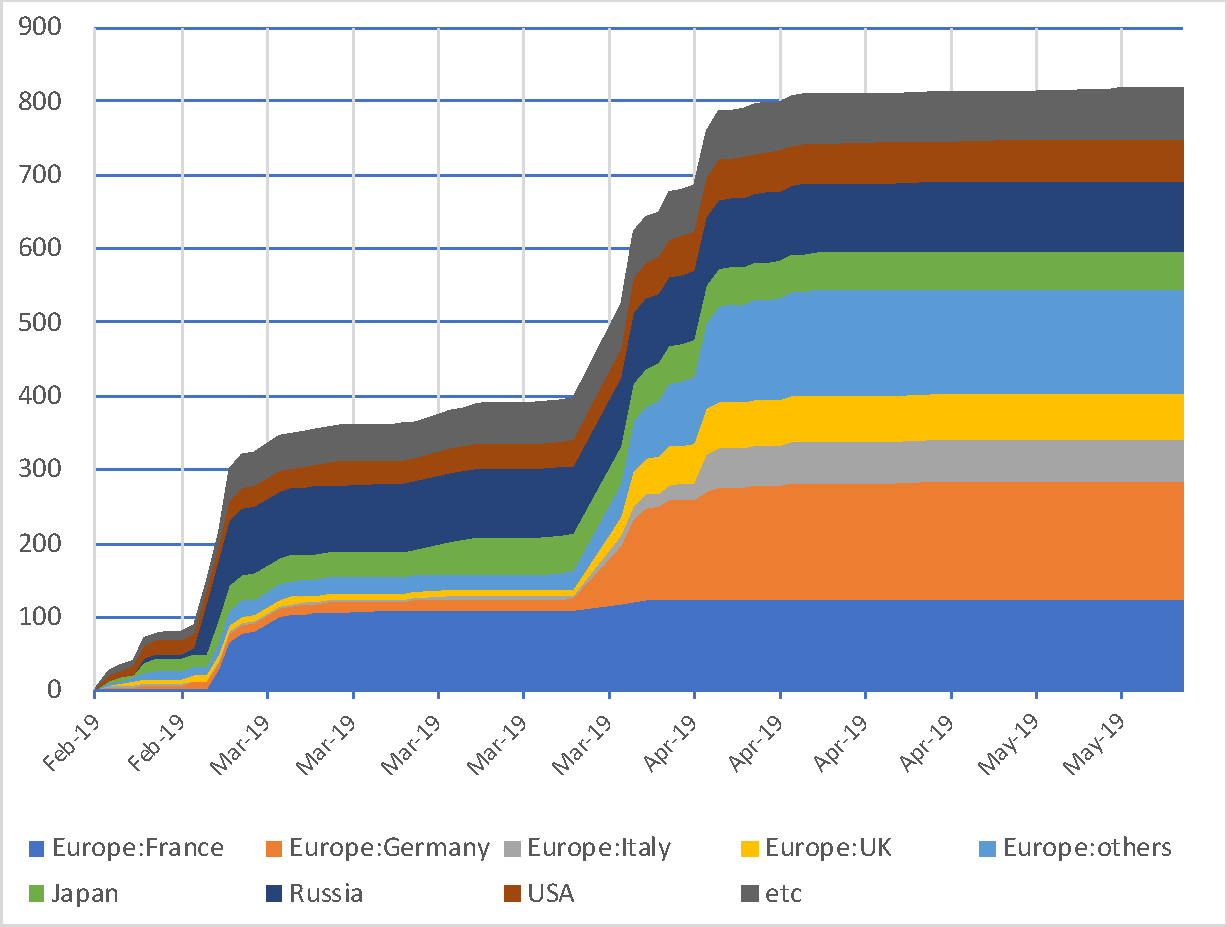
\includegraphics[width=8cm]{Figs/TimeSeries-Zoom.pdf}
    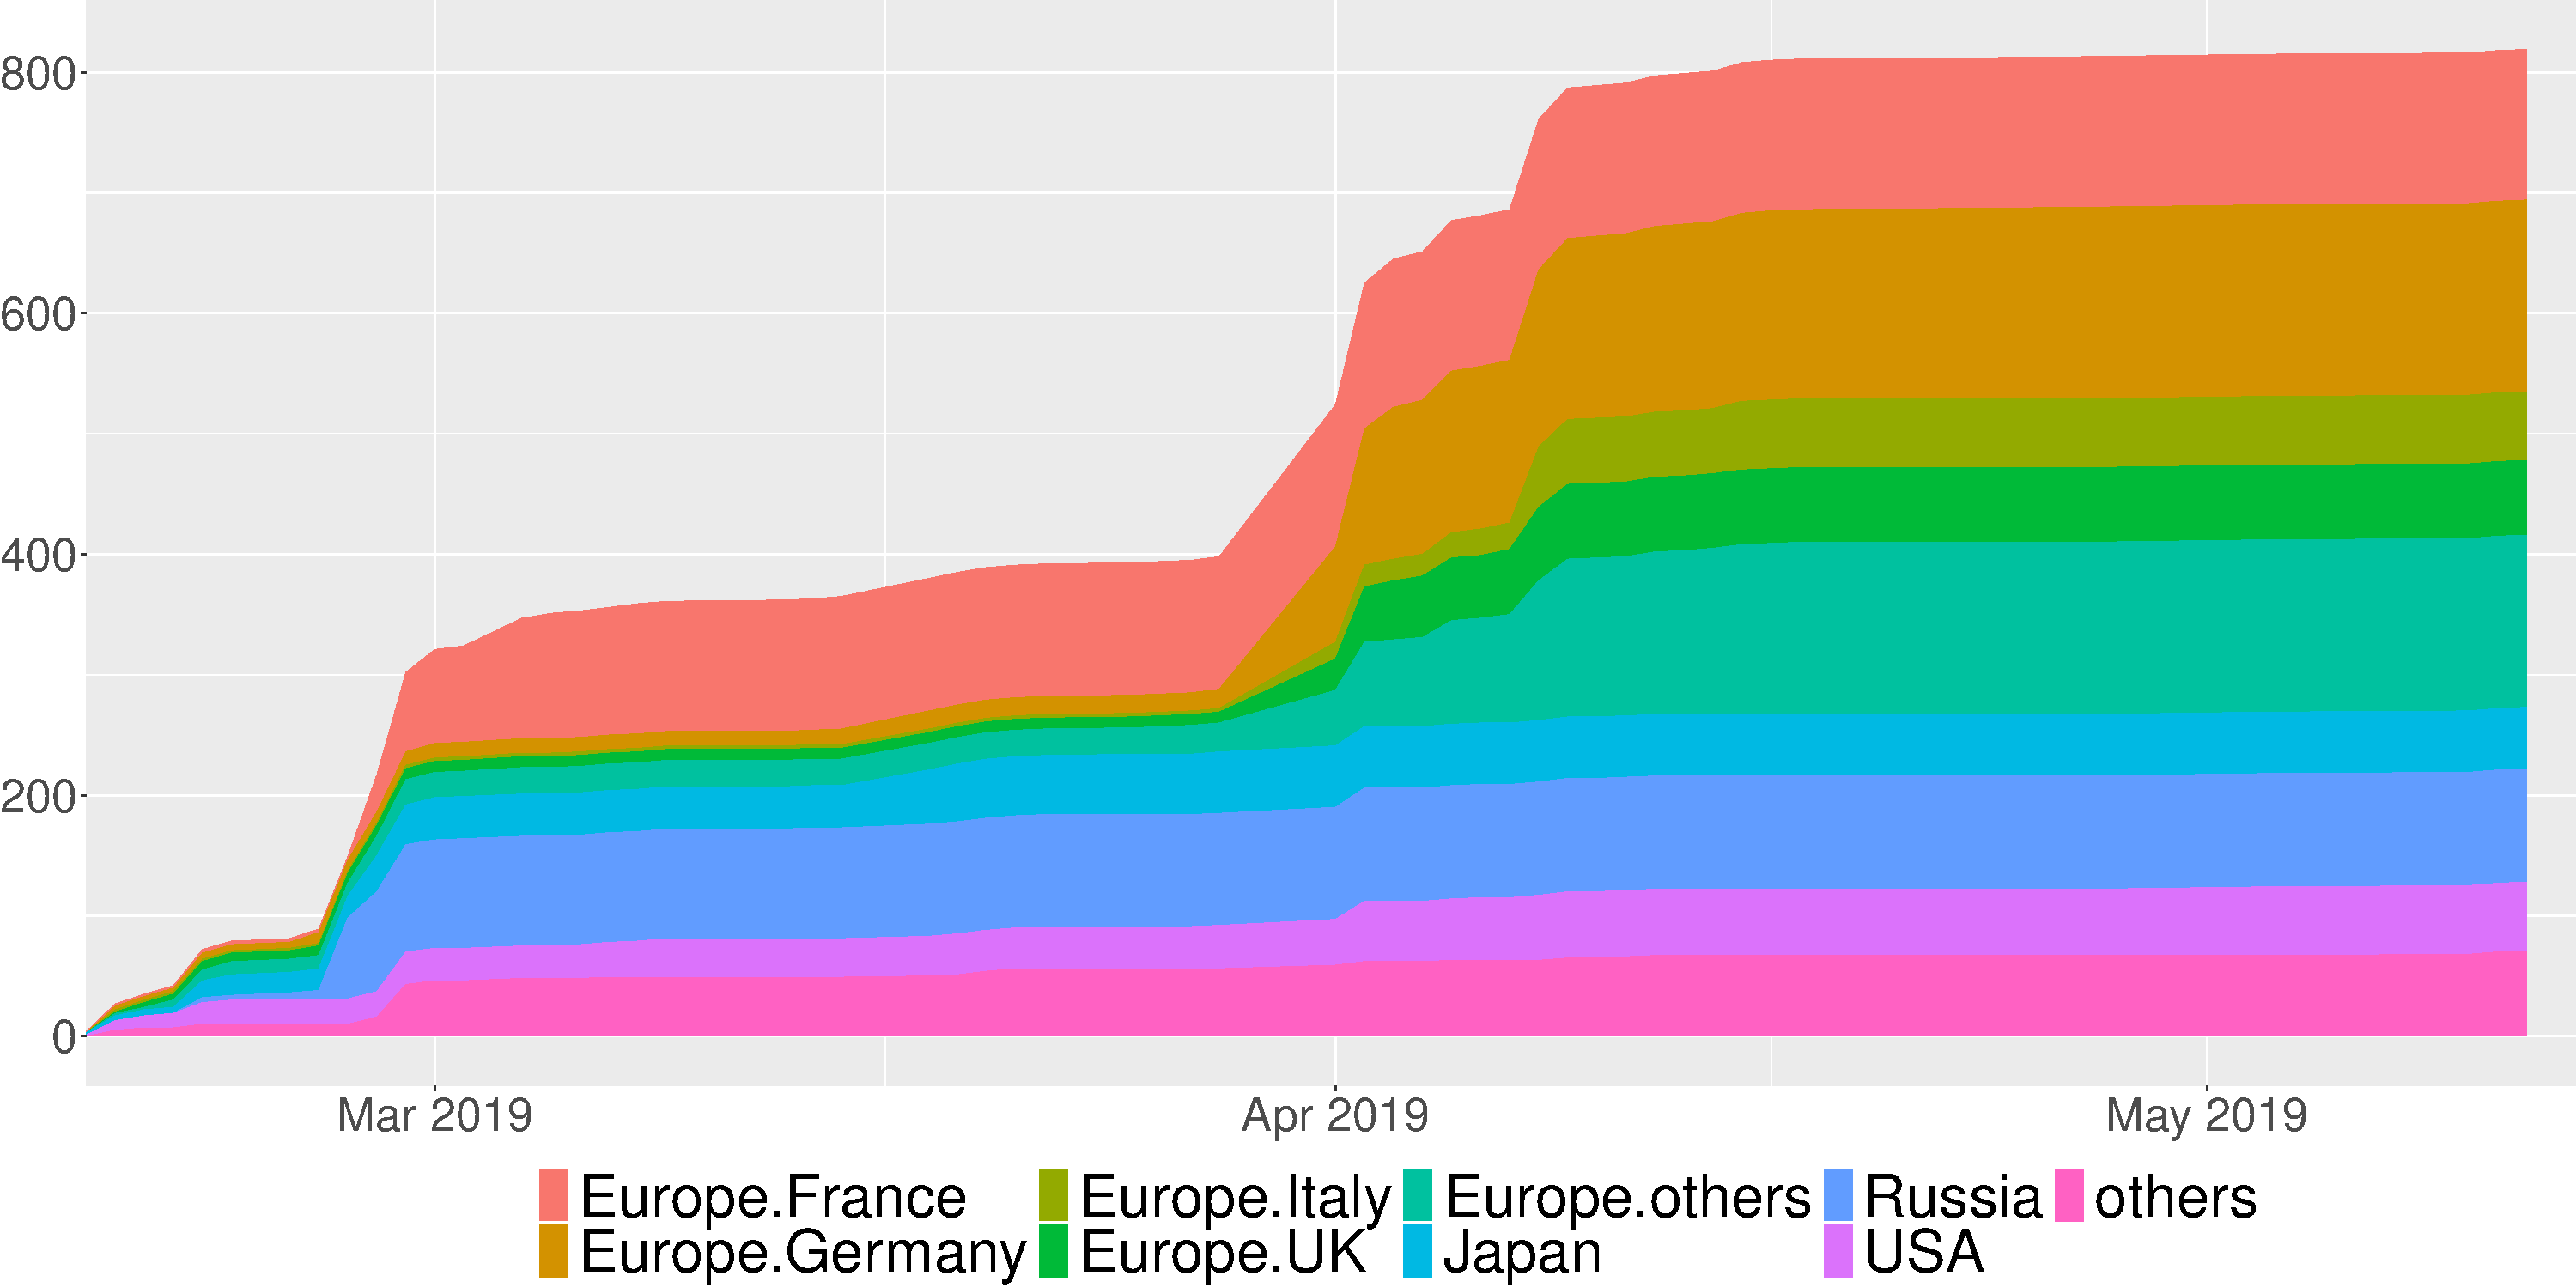
\includegraphics[width=8cm]{R-scripts/TimeSeries.pdf}
    \caption{Time series in first 90 days}
    \label{fig:time-series}
  \end{center}
\end{figure}

This local distribution strategy worked very well on some regions but
did not work universally. Table~\ref{tab:countries} shows the number
of participants of top 11 countries. In this report, the
countries having more than 50 participants are called {\it major
  countries} and are the objects of cross-tab analysis. There is a
trade-off between the number of participants of each major country
and the number of the major countries in the cross-tab analysis. The
threshold of 50 participants was selected to balance this trade-off
and it is not our intention of saying 50 is enough. Hence, some cross-tab
analysis may not be reliable enough.

Comparing with Table~\ref{tab:top500-share} listing the top 10
countries in the performance share in the Top500~\cite{Top500}, the
three major countries, USA, China and Japan, are not even the top 5 in
out survey. Especially China has only 18 participants including
Taiwan (2). We tried to increase the number of participants of those
countries, especially China, as much as we could, but we failed.
\comment{
  Once we asked a Chinese researcher why we could not get enough
  number off participants from China and his answer was because of their
  nationality.\todo[inline]{EJ: I do not understand why the nationality of chinese
    people is a problem for answering the survey. Please be more recise...}
}
%
\begin{table}[htb]%
  \begin{center}%
    \begin{tabular}[t]{cc}
      %
      \begin{minipage}[t]{0.5\hsize}
        \begin{center}%
          \caption{Top 11 Countries of Participants}%
          \label{tab:countries}%
          \begin{tabular}{c|l|r|r}%
            \hline%
            \# & Country & \#Ans & [\%] \\%
            \hline%
            1 & Germany 	& 159 & 18.7 \\%
            2 & France 	& 125 & 14.7 \\%
            3 & Russia 	& 94  & 11.1 \\%
            4 & UK 		& 67  &  7.9 \\%
            5 & Japan 	& 64  &  7.5 \\%
            6 & USA 	& 58  &  6.8 \\%
            7 & Italy 	& 57  &  6.6 \\%
            \hline%
            8 & Switzerland & 40  &  5.8 \\%
            9 & South Korea & 27  &  3.2 \\%
            10 & Austria 	& 26  &  3.1 \\%
            11 & China (+Taiwan) & 18 & 2.1 \\%
            \hline%
            \multicolumn{4}{c}{42 countries, 851 participants} \\%
          \end{tabular}%
        \end{center}%
      \end{minipage}
      %
      \begin{minipage}[t]{0.5\hsize}
        \begin{center}%
          \caption{Top500 Performance Share (June 2020)}%
          \label{tab:top500-share}%
          \begin{tabular}{c|l|r}%
            \hline%
            \# & Country & [\%] \\%
            \hline%
            1  & USA 	  & 28.2 \\%
            2  & China 	  & 25.6 \\%
            3  & Japan 	  & 23.9 \\%
            4  & Italy	  & 4.0  \\%
            5  & France	  & 3.6  \\%
            6  & Germany 	  & 3.1  \\%
            7  & UK		  & 1.4  \\%
            8  & Canada	  & 1.3  \\%
            9  & Netherlands  & 1.1  \\%
            10 & Switzerland  & 1.1  \\%
            \hline%
          \end{tabular}%
        \end{center}%
      \end{minipage}%
      %
    \end{tabular}%
  \end{center}%
\end{table}%
%
% Profile
%
Fig.~\ref{fig:occupations} shows the graph of Q1 asking participants'
occupation. As shown, roughly 80\% of participants are working at 
universities or governmental research institutes.
%
\begin{figure}[htb]
  \begin{center}
    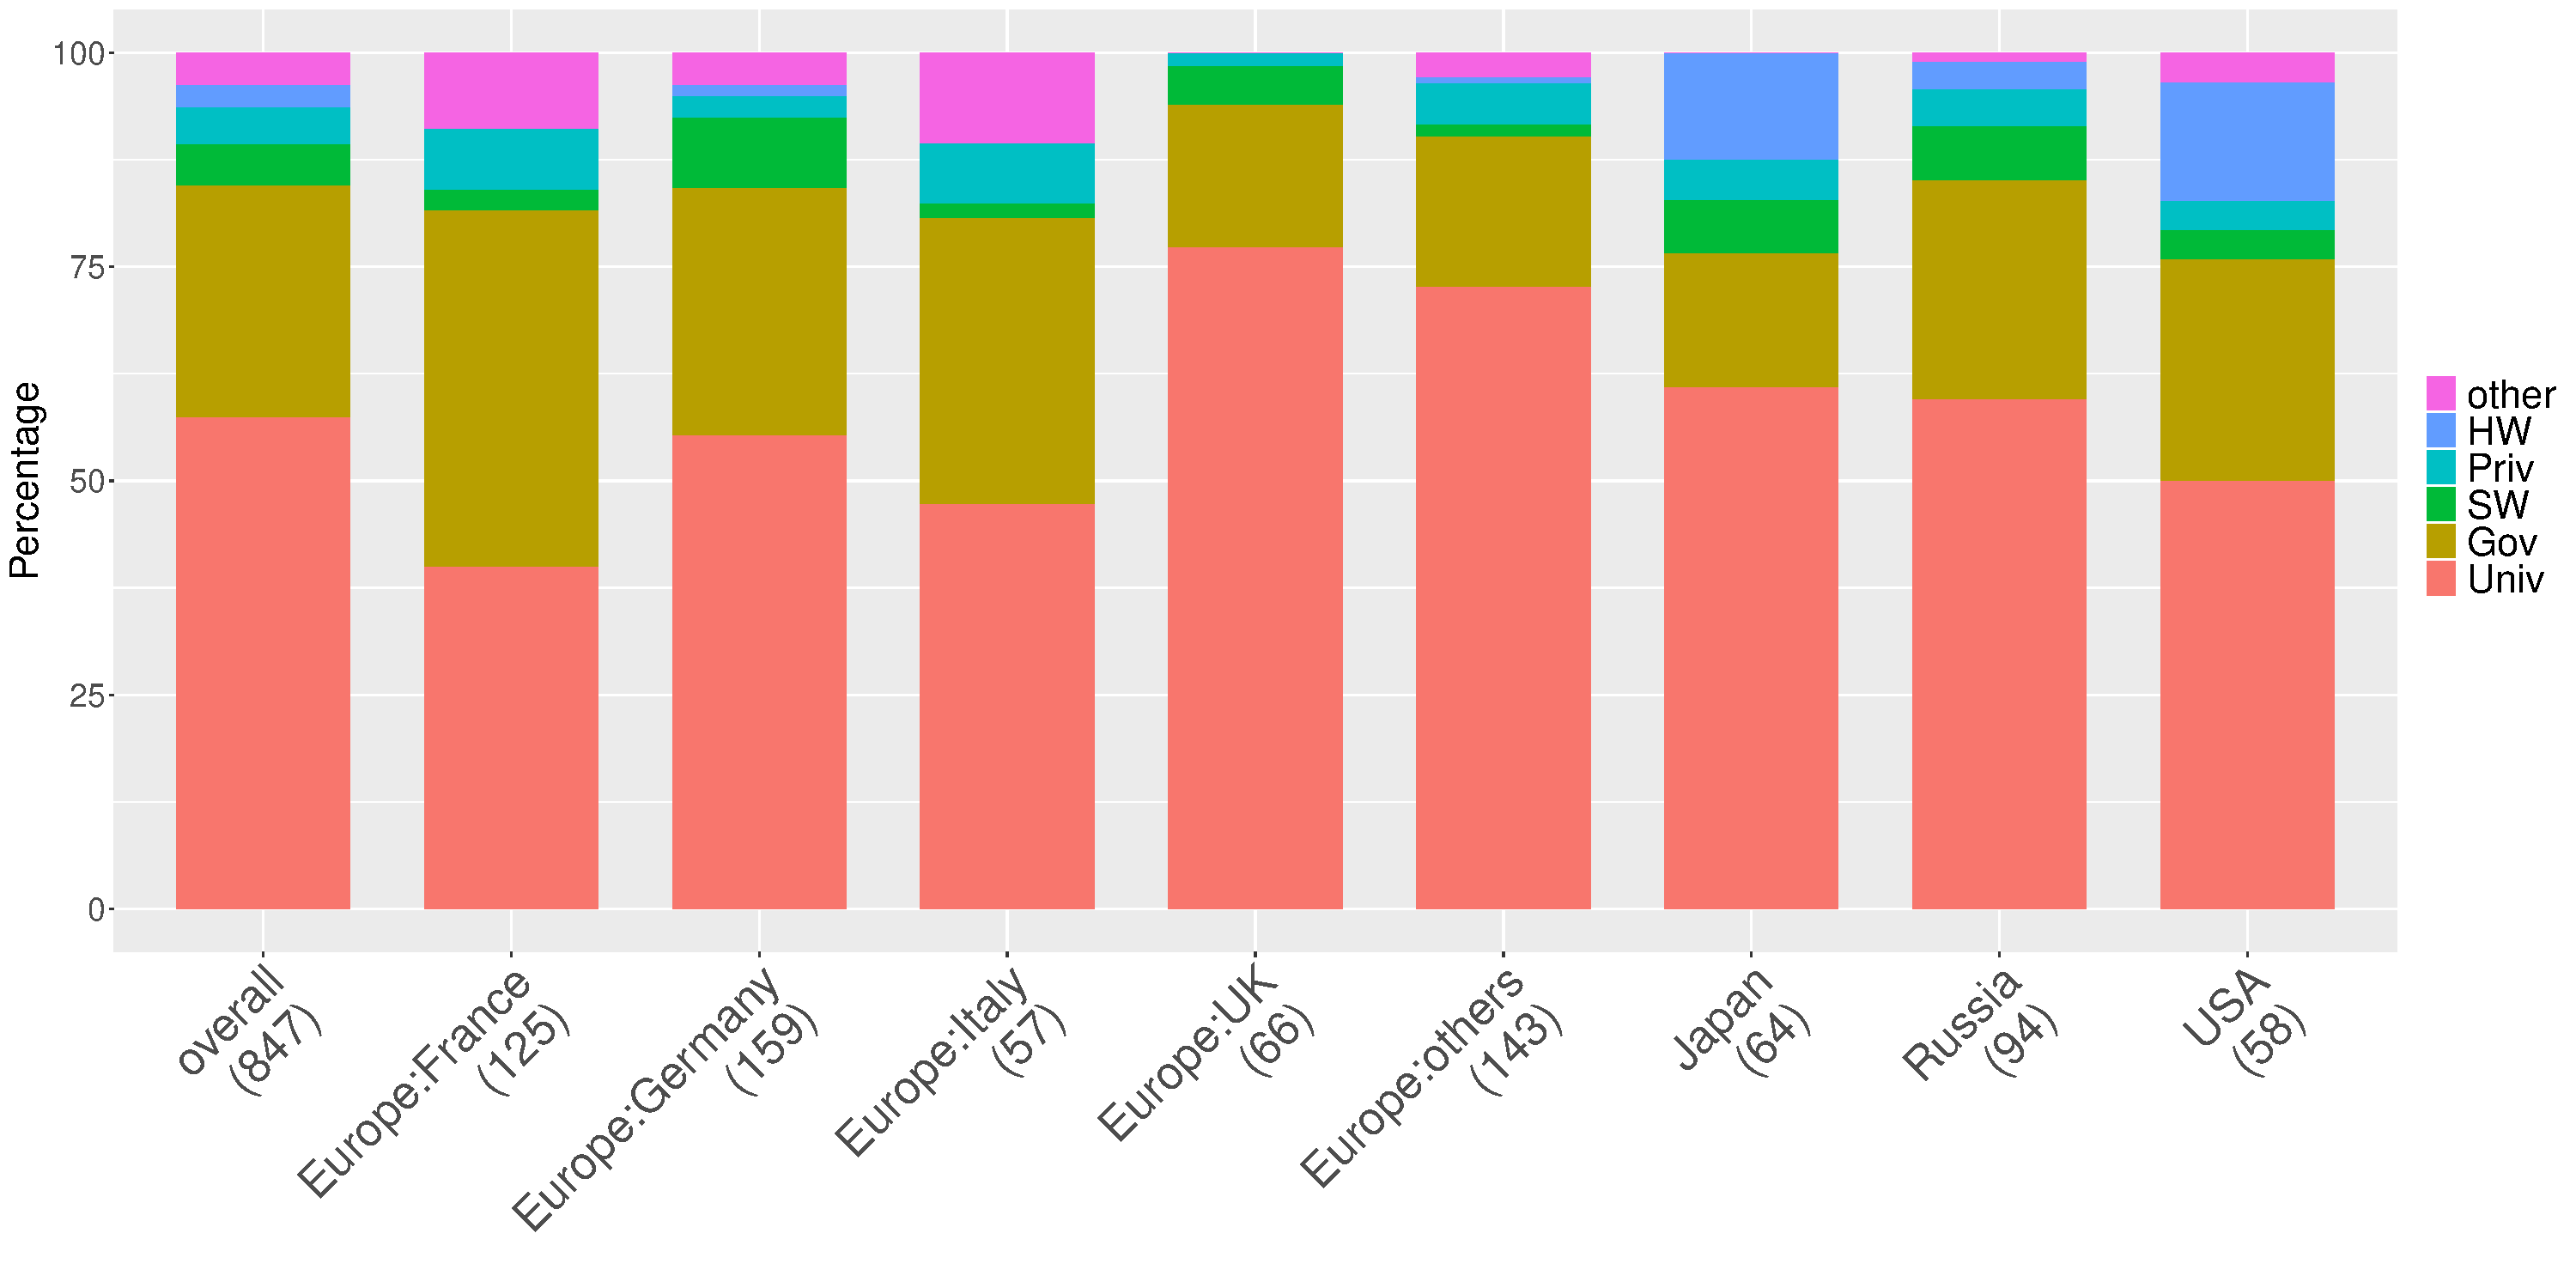
\includegraphics[width=8cm]{R-scripts/Q1.pdf}
    \caption{Q1: Occupations {\it(single)}}
    \label{fig:occupations}
  \end{center}
\end{figure}

Fig.~\ref{fig:working-fields} shows the result of asking ``Which
fields are you mostly working in?'' Generally speaking, most
participants are working on numerical applications and/or
libraries. In Japan and US, the percentages of parallel languages and
OS/runtimes are higher than the other countries and regions.

\begin{figure}[htb]
  \begin{center}
    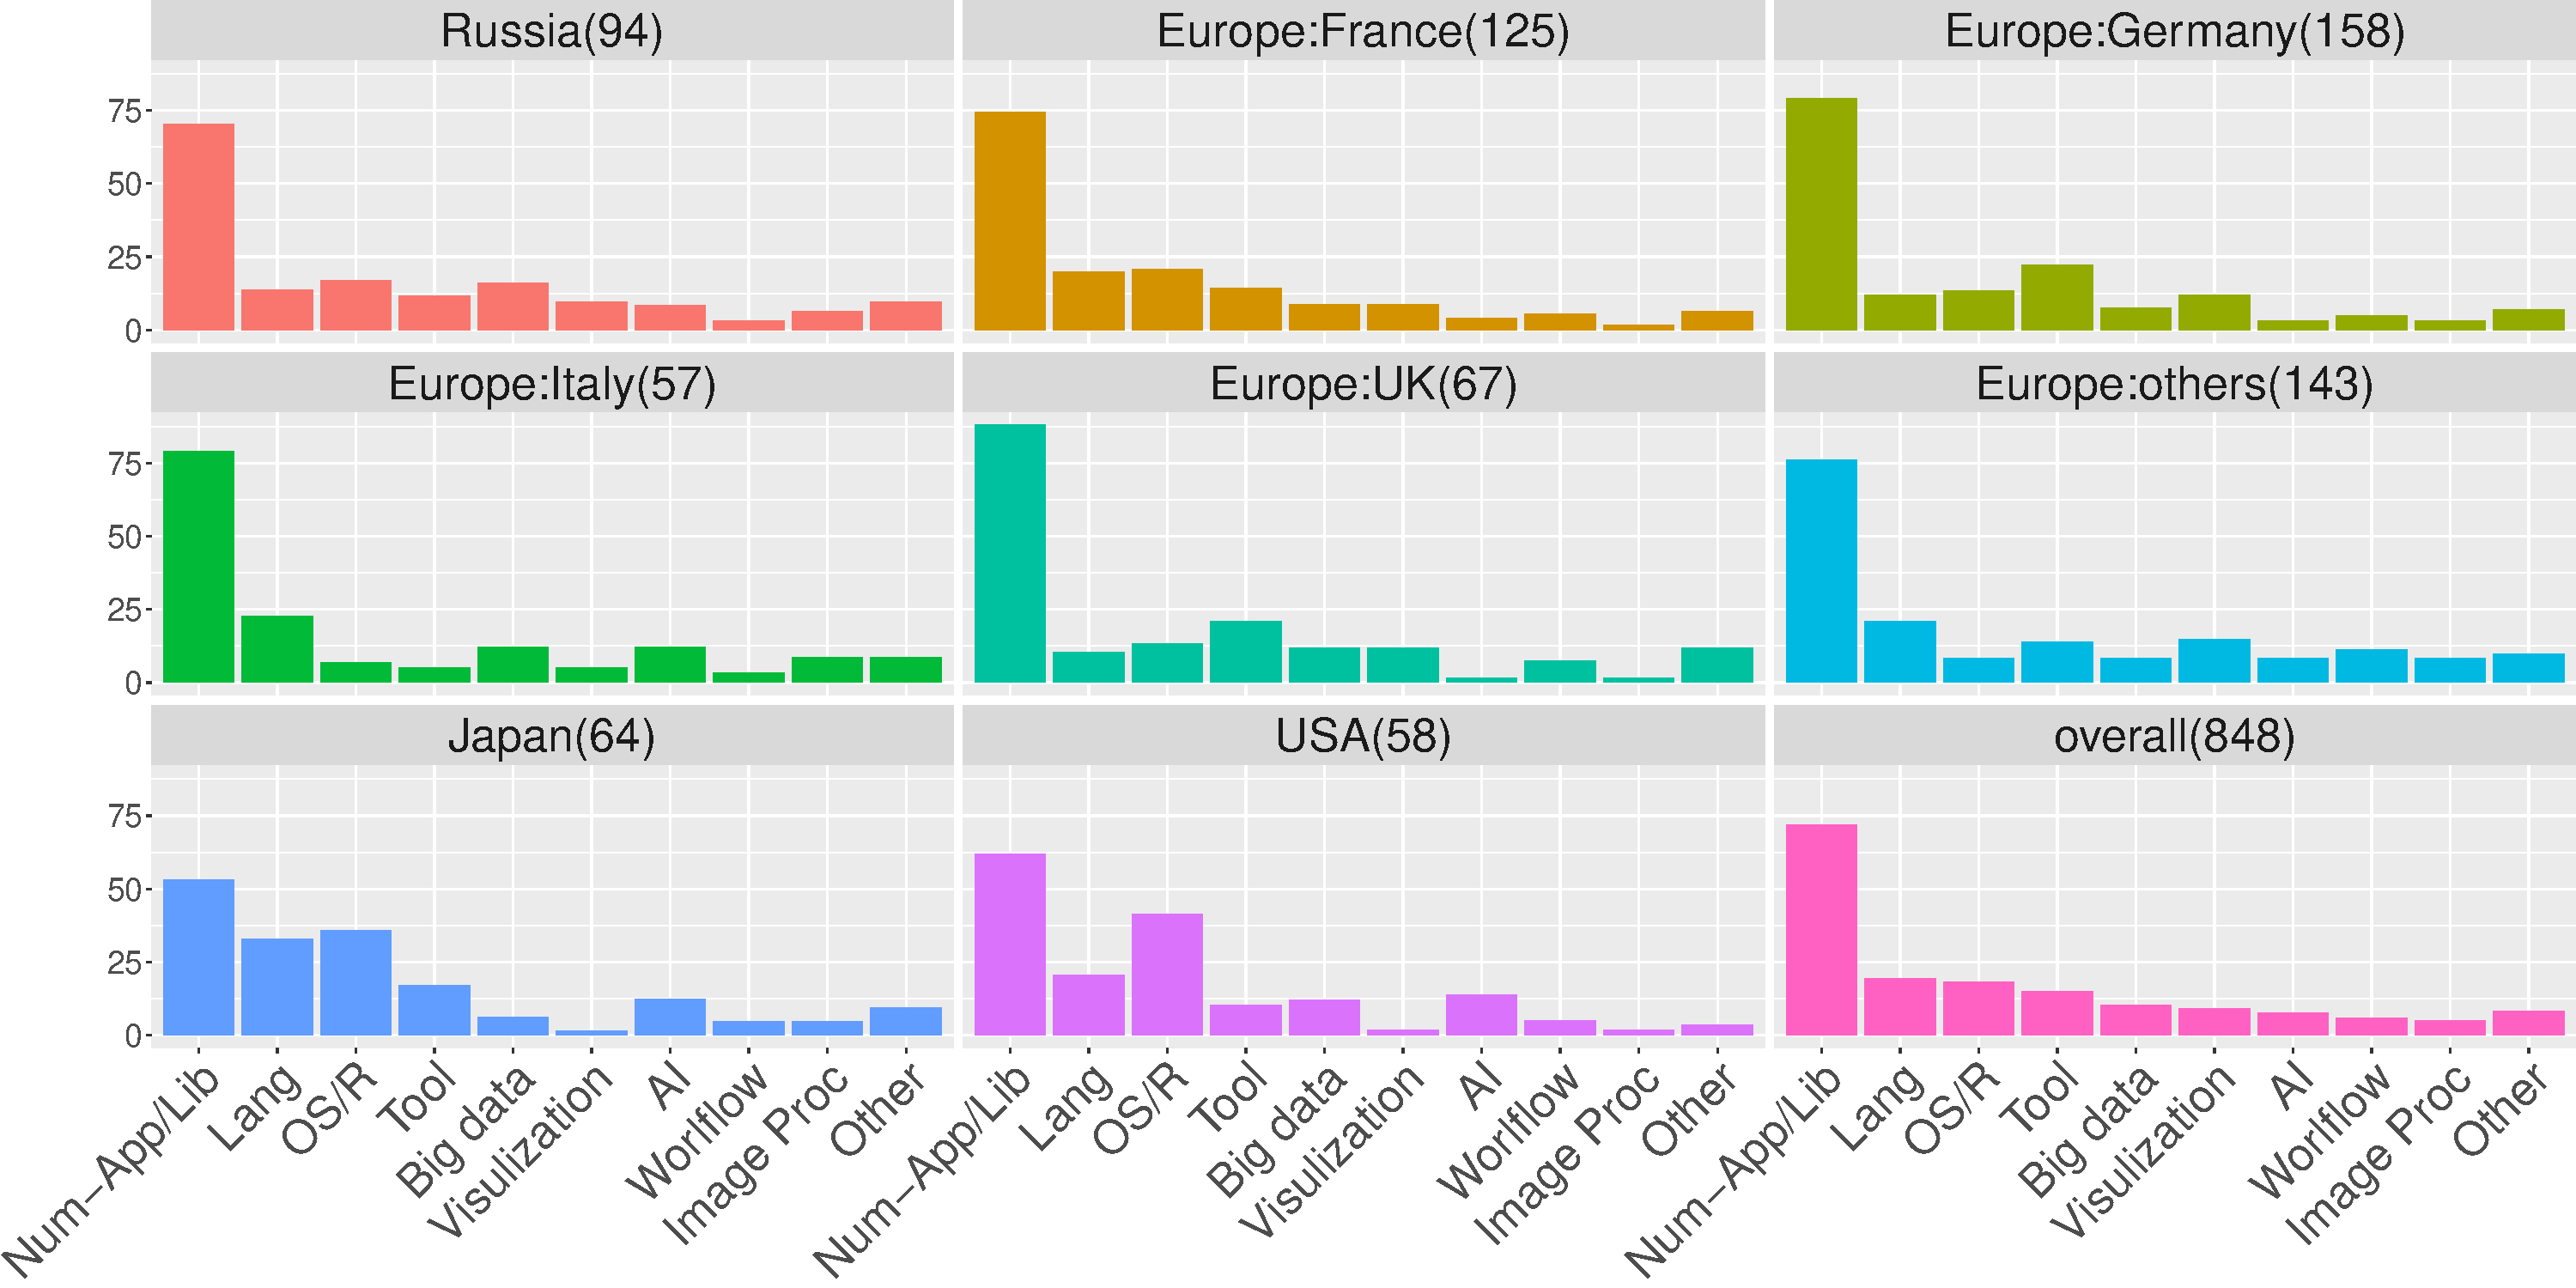
\includegraphics[width=8cm]{R-scripts/Q7.pdf}
    \caption{Q7: Working Fields {\it(multiple)}}
    \label{fig:working-fields}
  \end{center}
\end{figure}

\section{Comparison with the ECP survey}

Although the ECP questionnaire and our questionnaire were designed
independently, there are several questions quite similar. It is also
assumed that some of the participants of our survey 
also participated in the ECP survey. However, significant differences
between them can be found. Before going into the details, we clarify
some profiles of the participants in our survey.

\begin{figure}[htb]
  \begin{center}
    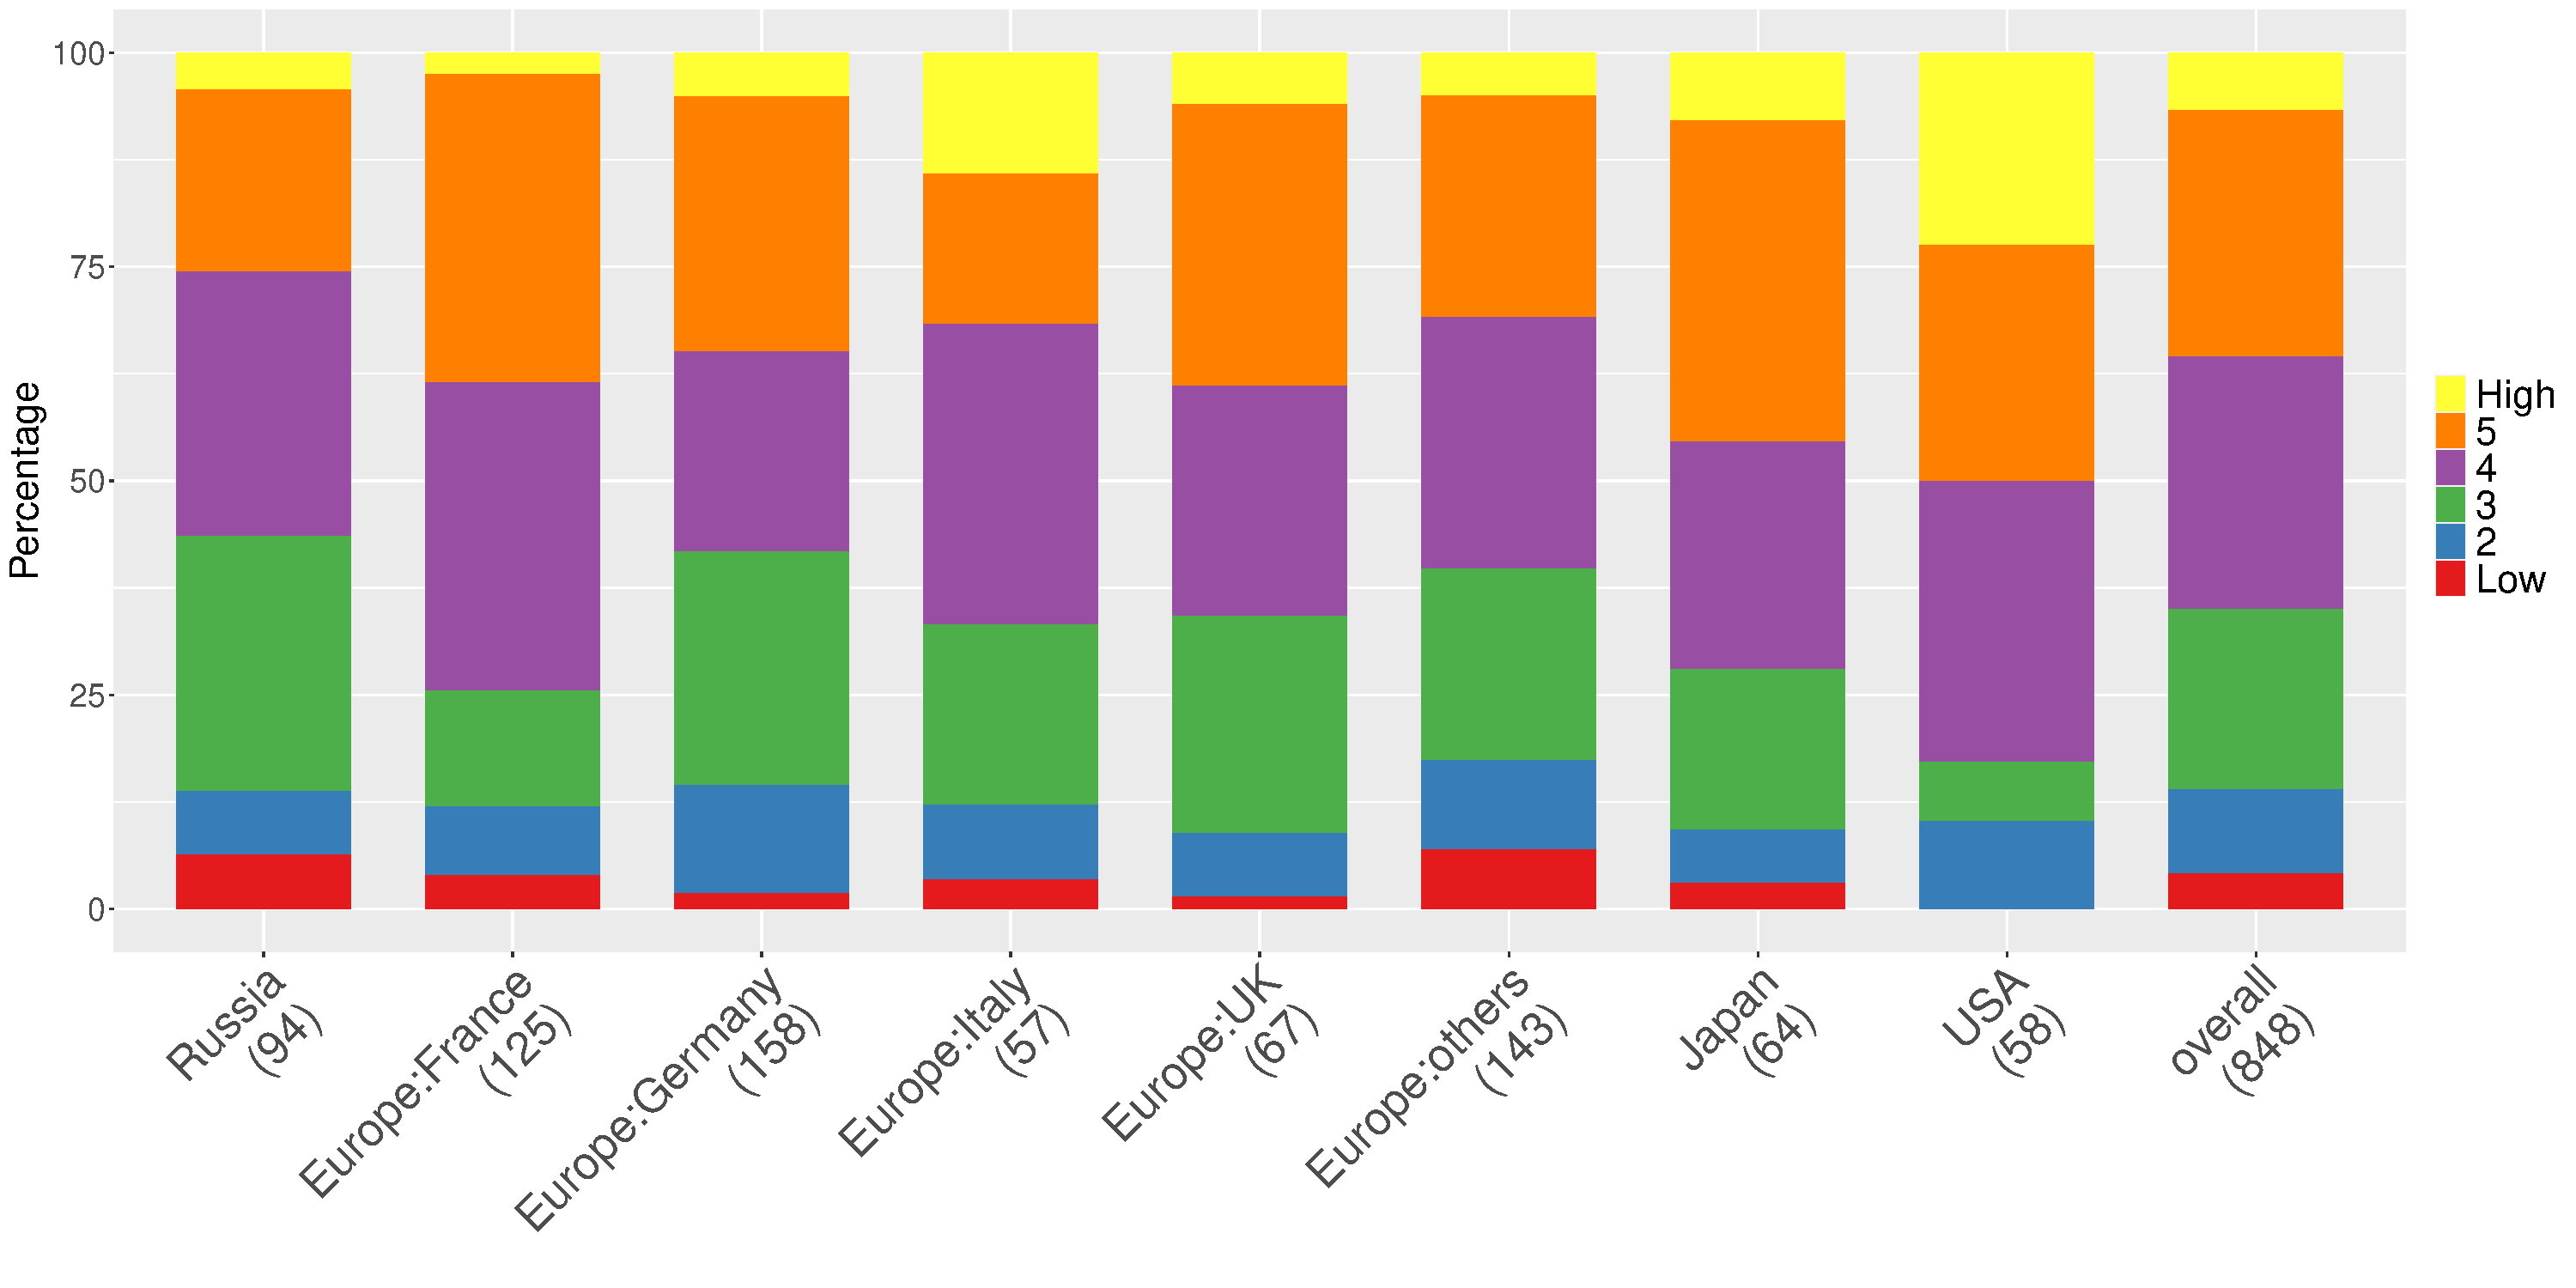
\includegraphics[width=8cm]{R-scripts/Q3.pdf}
    \caption{Q3: Self assessment of MPI Skill {\it(single)}}
    \label{fig:mpi-skill}
  \end{center}
\end{figure}

We assumed that the participants in the ECP survey have more
experiences on MPI
programming than the participants of ours. Fig.~\ref{fig:mpi-skill} 
shows the results of Q3 asking to rate the participants MPI skill by
themselves in our survey.  In the US case 
\footnote{Note that we asked
  the workplace in past 5 years, not asking nationalities.}
(right most bar), almost half of participants rate 5 or 6
(6 is the highest). This percentage in having high MPI skill (larger
than or equal to 5) in the US is the highest among the other
countries and nobody in US marked the lowest skill.

\begin{figure}[htb]
  \begin{center}
    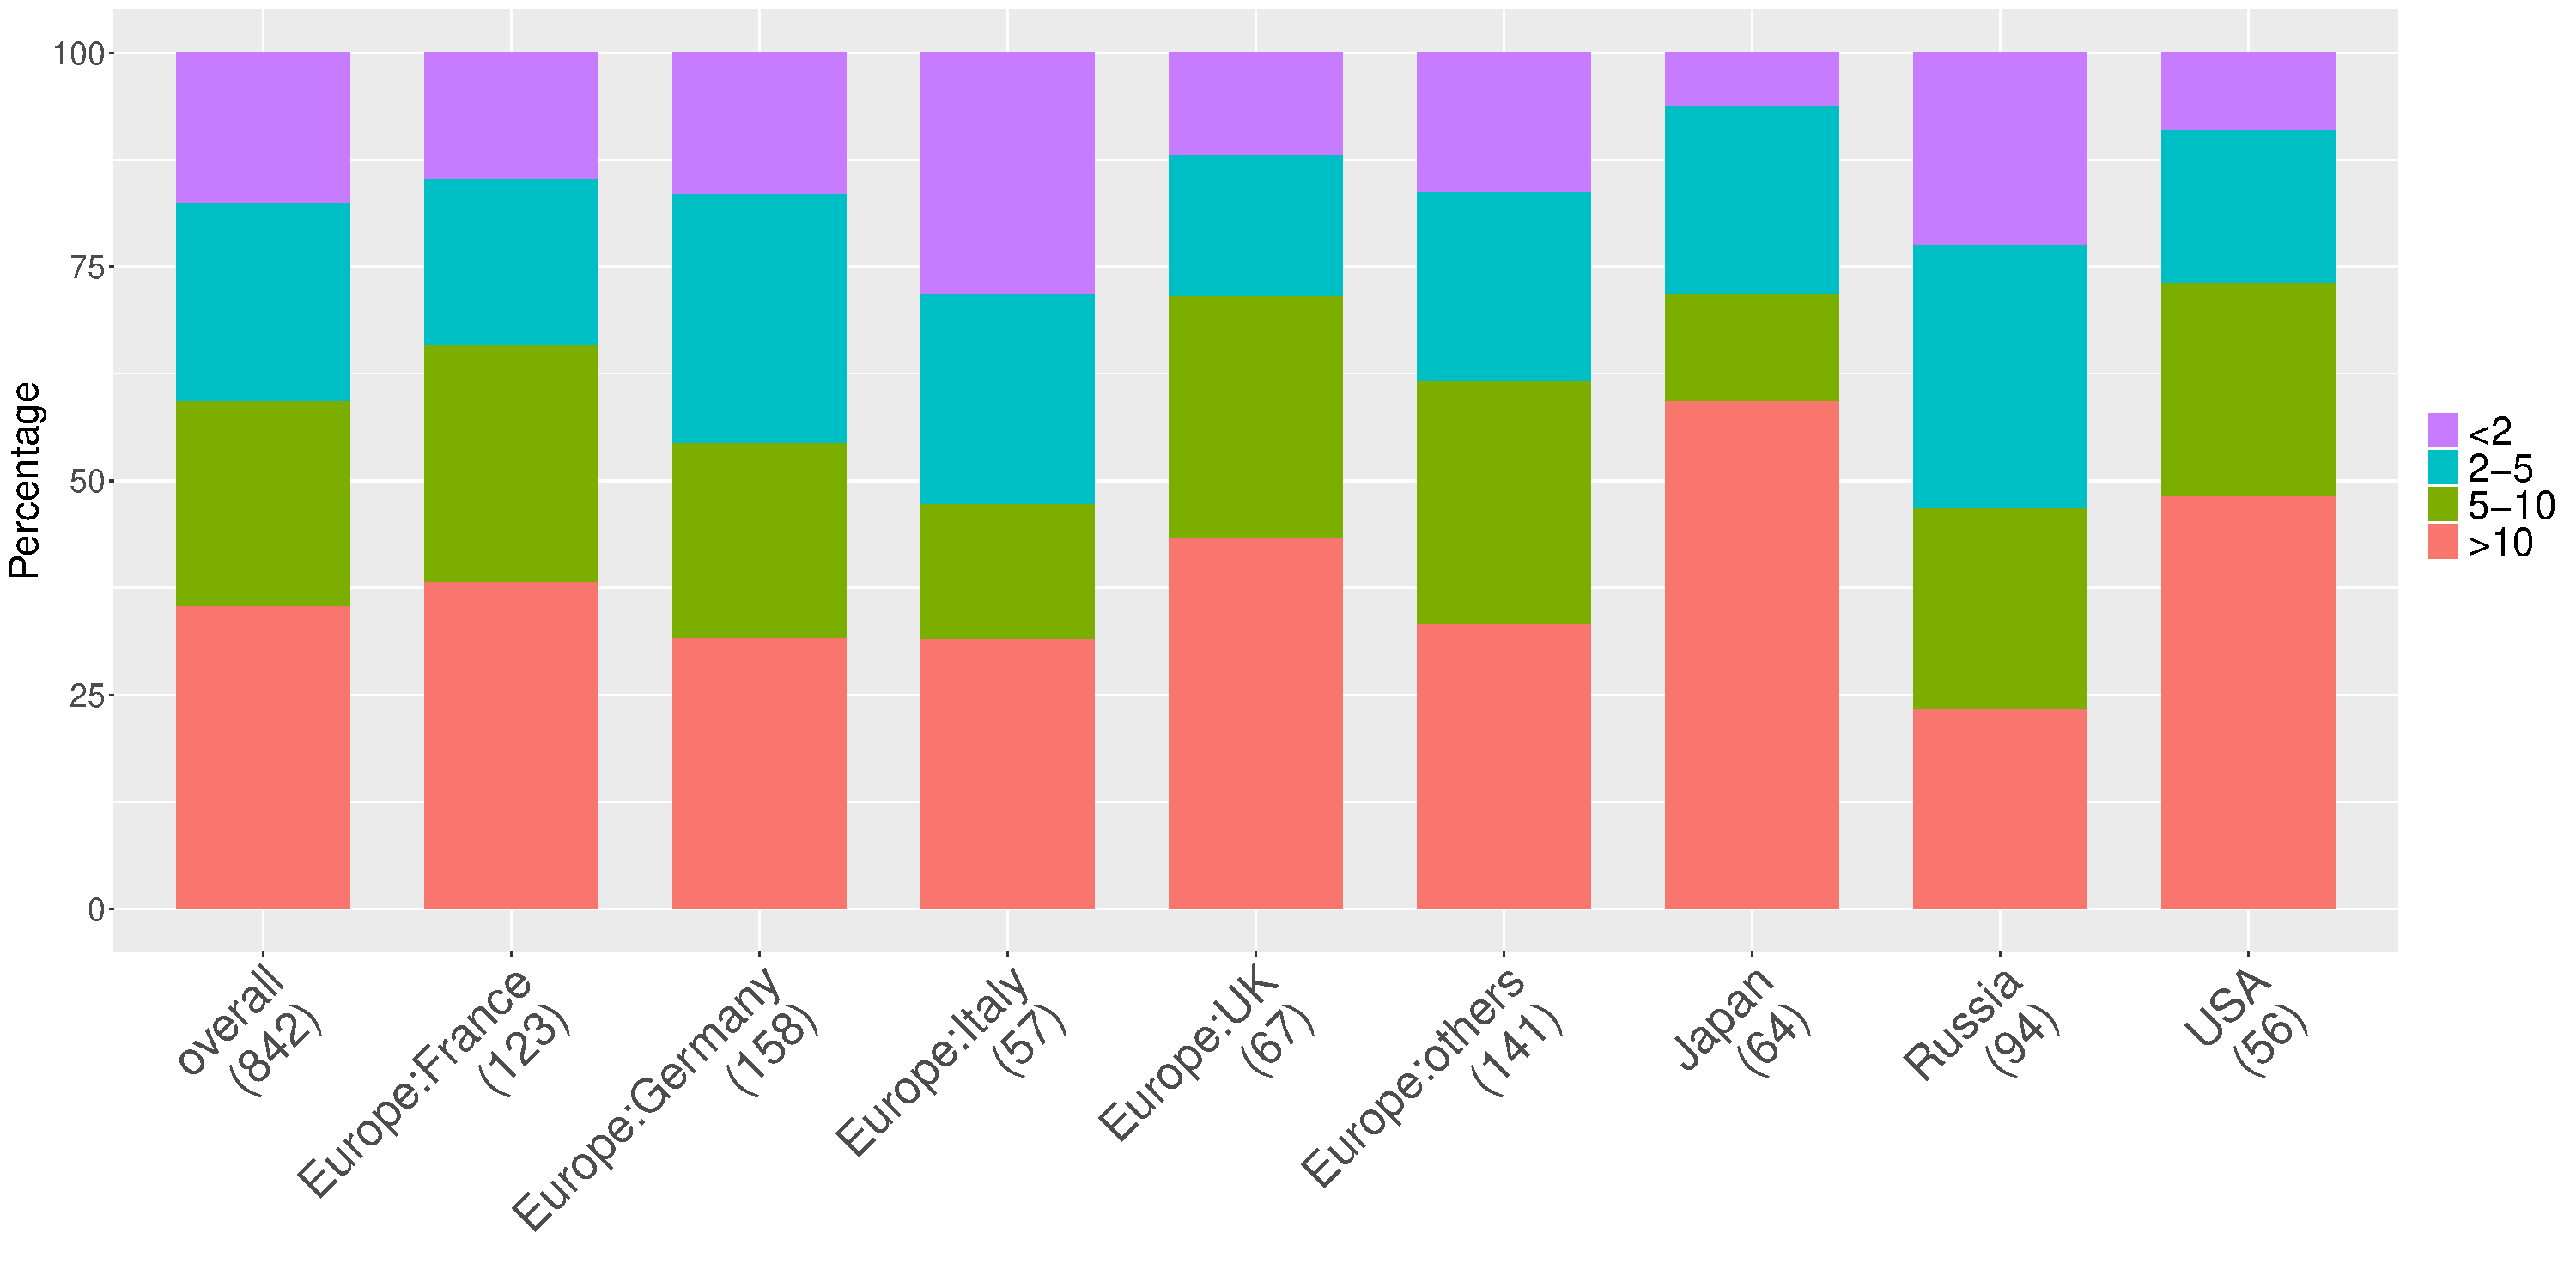
\includegraphics[width=8cm]{R-scripts/Q6.pdf}
    \caption{Q6: MPI Experience {\it(single)}}
    \label{fig:mpi-experience}
  \end{center}
\end{figure}

Fig.~\ref{fig:mpi-experience} shows the more interesting result. This
graph is the result of asking ``How long have you been writing MPI
programs?'' and the choices are 'more than 10 years' (denoted as
\myquote{\textgreater 10}), \myquote{between 5 and 10 years}
(denoted as \myquote{5-10}), \myquote{between 2 and 5 years}
(denoted as \myquote{2-5}) and \myquote{less than 2 years} 
(denoted as \myquote{\textless 2}).
Interestingly 9\% of US participants have less than 2 years MPI
experience, but they do no rank their MPI expertise the lowest (Fig.~\ref
{fig:mpi-skill}). Japan followed by USA has the highest percentage in
more than 10 years and has the lowest percentage in less than 2 years
experience. Russia followed by Italy has the highest percentage in
less than 5 years experience (including the less than 2 years
experience case). 

We chose three questions from both of out survey and ECP survey that
are very similar and thus the results are comparable
(Table~\ref{tab:comparable-questions}). We will discuss those results
in the following subsections.

\begin{table}[htb]%
  \begin{center}%
    \caption{Comparable Questions}%
    \label{tab:comparable-questions}%
    \begin{tabular}[t]{c|c}
      \hline
      \multicolumn{2}{c}{A. Layering MPI calls} \\
      \hline
      \begin{minipage}[t]{0.45\hsize}
        Q21: In most of your programs, do you pack MPI function calls into
        their own file or files to have your own abstraction layer for
        communication?  {\it(single)}
      \end{minipage}
      &
      \begin{minipage}[t]{0.45\hsize}
        Q22: Do you have an abstraction layer that hides the MPI calls? Or do
        most of your developers write MPI calls directly? {\it(single)}
      \end{minipage}
      \\
      \hline
      \multicolumn{2}{c}{B. Using MPI Aspects} \\
      \hline
      \begin{minipage}[t]{0.45\hsize}
        Q17: What aspects of the MPI standard do you use in your program in its
        current form? {\it(multiple)}
      \end{minipage}
      &
      \begin{minipage}[t]{0.45\hsize}
        Q35: What aspects of the MPI standard do you use in your application in
        its current form? {\it(multiple)}
      \end{minipage}
      \\
      \hline
      \multicolumn{2}{c}{C. Multi-threading} \\
      \hline
      \begin{minipage}[t]{0.45\hsize}
        Q18: Which MPI thread support are you using? {\it(multiple)}
      \end{minipage}
      &
      \begin{minipage}[t]{0.45\hsize}
        Q59: Which MPI threading option are you using? {\it(single)}
      \end{minipage}
      \\
      \hline
      Our Survey & ECP Survey \\
      \hline
    \end{tabular}%
  \end{center}%
\end{table}%

\subsection{Layering MPI calls}

\begin{figure}[htb]
  \begin{center}
    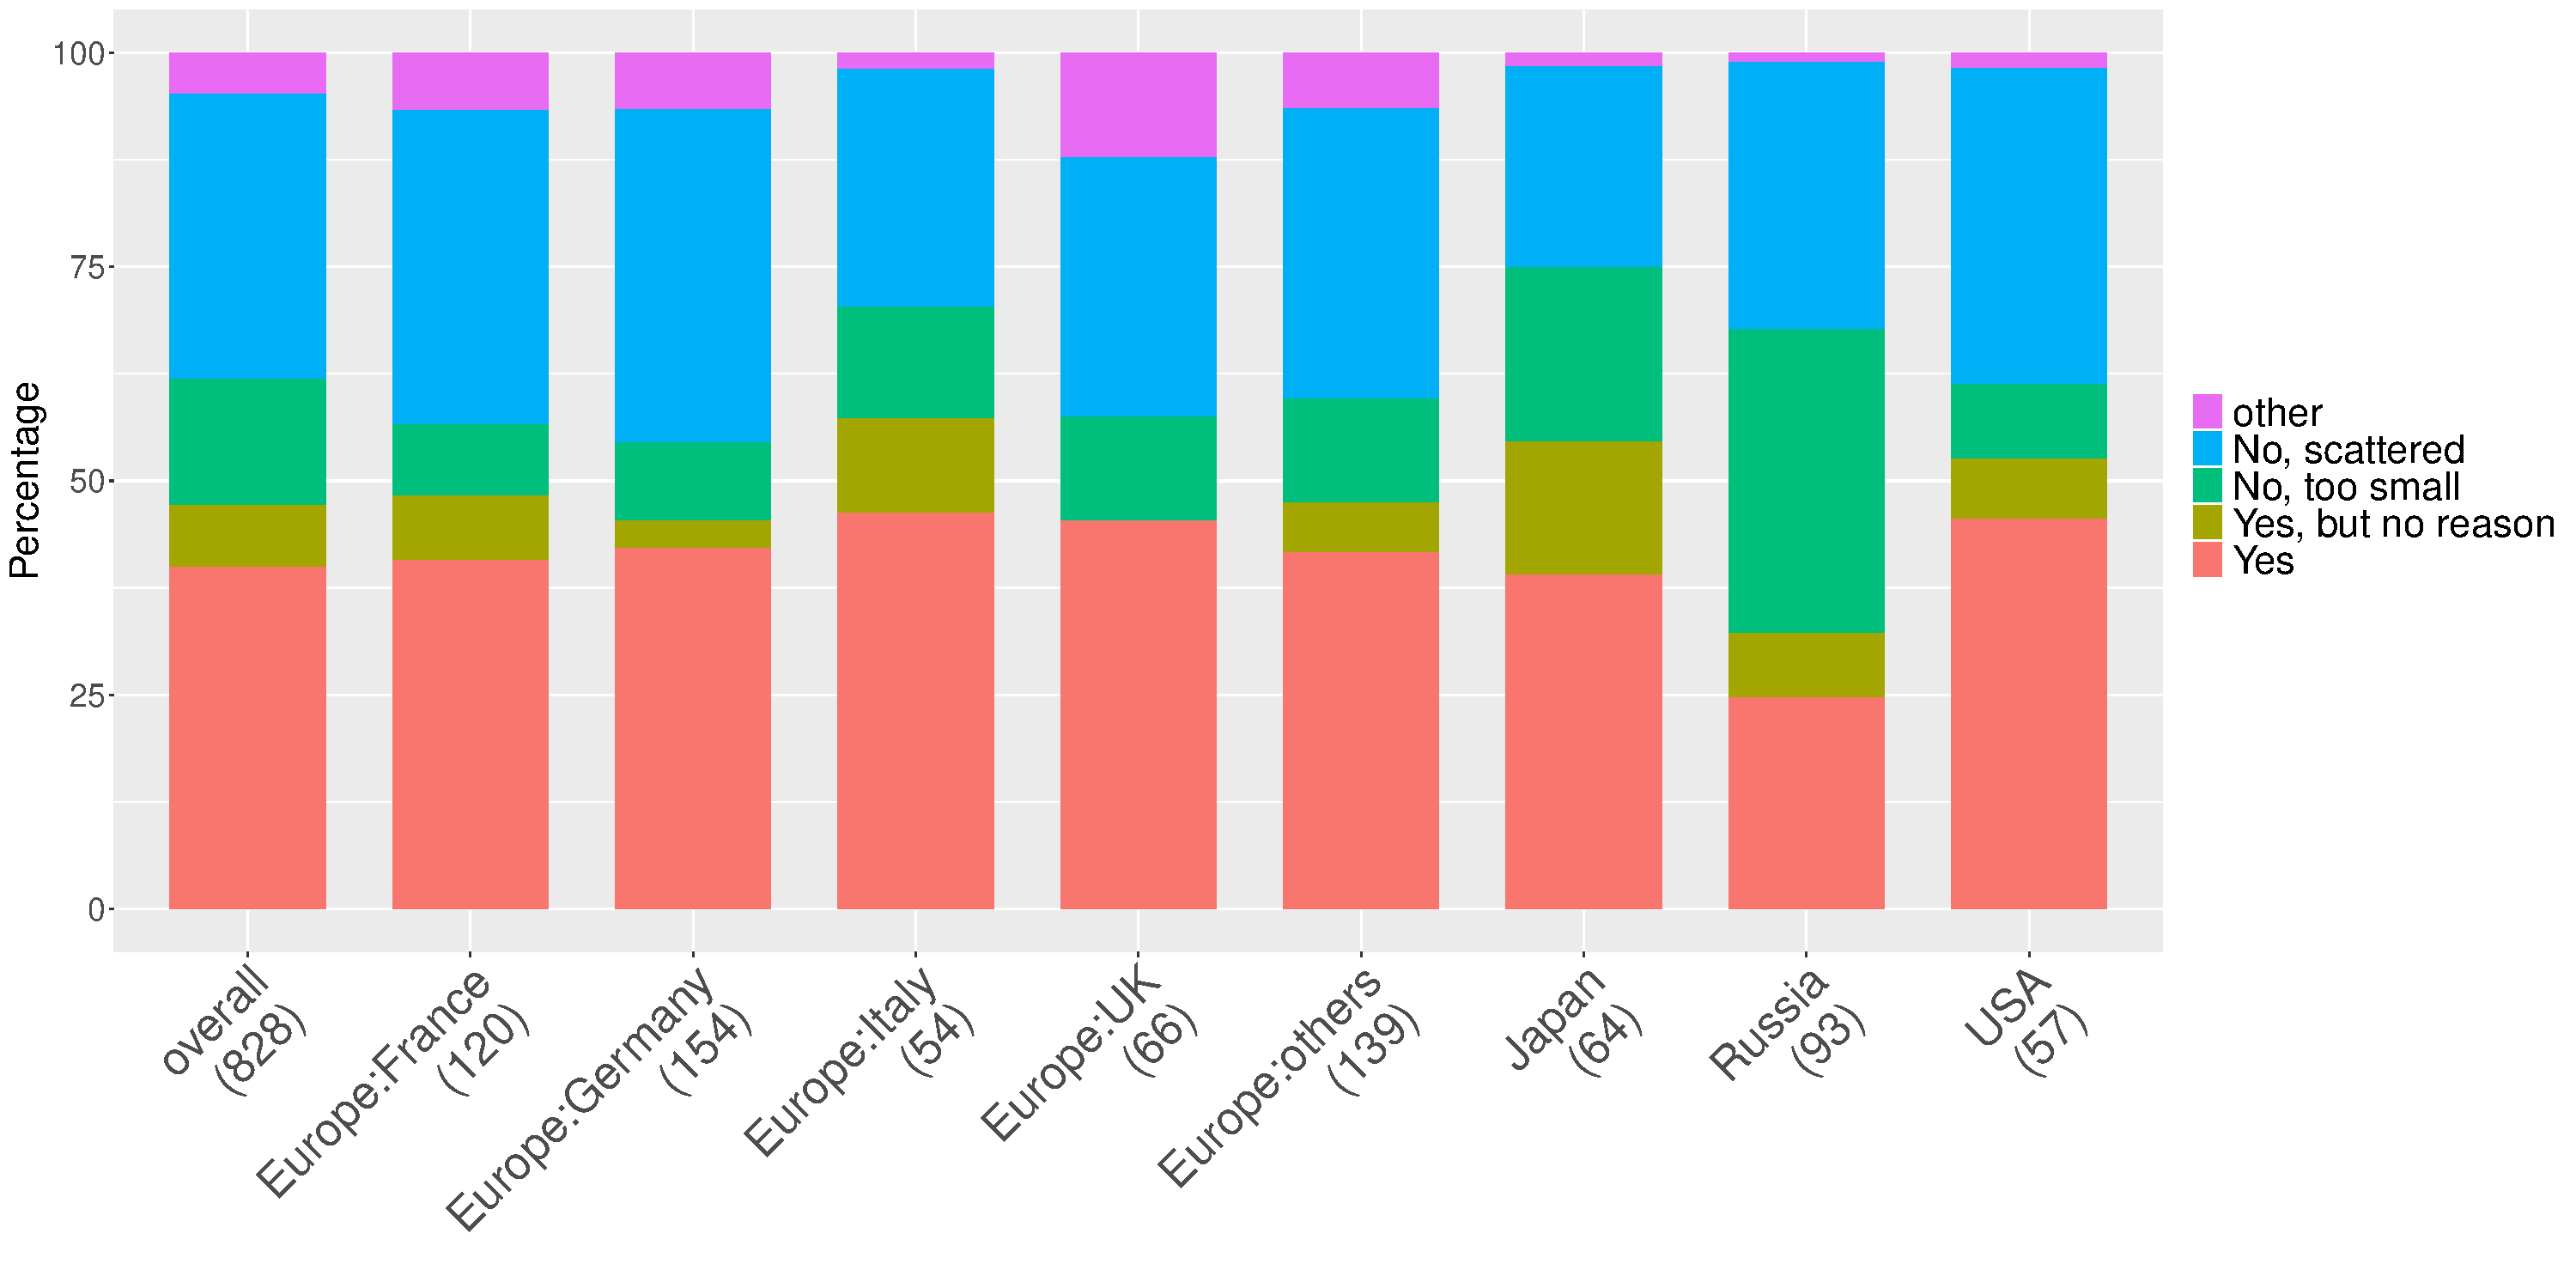
\includegraphics[width=8cm]{R-scripts/Q21.pdf}
    \caption{Q21: Layering MPI calls {\it(single)}}
    \label{fig:layering-mpi-calls}
  \end{center}
\end{figure}

Fig.~\ref{fig:layering-mpi-calls} shows the result of our survey and
Table~\ref{tab:layering-mpi-calls} shows the comparison between ours
and ECP survey. In the ECP survey, the participants are categorized
into two groups; application development (AD) and system technology
(ST). It is interesting that the percentage in packing MPI calls
in our survey is roughly 50\% even in the US, whilst the ratio of yes
and no is approximately $6:4$ in the ECP survey.
Having a closer look at Fig.~\ref{fig:layering-mpi-calls}, the answer,
\myquote{No, my program is too small to do that,} dominates in Russia. In
the other countries, the participants having a packing layer occupies
40-50\%. 

\begin{table}[htb]%
  \begin{center}%
    \caption{Layering MPI calls}\label{tab:layering-mpi-calls}%
    \begin{tabular}{c|c||c|c||c|c|c}%
      \hline%
      \multicolumn{2}{c||}{Choice} & \multicolumn{2}{c||}{Our Survey [\%]} &
      \multicolumn{3}{c}{ECP [\%]} \\
      \cline{3-7}%
      \multicolumn{2}{c||}{} & overall & USA & AD & ST & AD+ST \\
      \hline%
      \hline%
      Yes & - & 40 & 46 & & & \\
      & no reason & 7 & 7 & & & \\
      \cline{2-4}%
      & (sum) & 47 & 53 &  79 & 46 & 62 \\
      \hline%
      \hline%
      No & too small & 15 & 9 & & & \\
      & - & 33 & 37 & & & \\
      \cline{2-4}%
      & (sum) & 48 & 46 & 21 & 54 & 38 \\
      \hline%
      Other & - & 5 & 2 & - & - & - \\
      \hline%
    \end{tabular}%
  \end{center}%
\end{table}%

\subsection{Using MPI Aspects}

The question asking ``What aspects of the MPI standard do you use in
your application in its current form?'' in the ECP survey and Q17 of
our survey are almost equivalent
questions, although choices are somewhat
different. Fig.~\ref{fig:using-mpi-aspects} shows the result of our 
survey and Table~\ref{tab:using-mpi-aspects} shows the comparison
between ECP and ours. As shown in Fig.\ref{fig:using-mpi-aspects}, the
using aspects can be categorixed in three groups; A) more frequently
used (point-to-point and collectives), B) second frequently used
(datatypes, with OpenMP, communicator, and one-sided), and C) less
frequently used (PMPI, persistent, and dynamic process (denoted as
\myquote{dyn. process}).
It should be noted that all these less frequently used features were
already introduced and standardized in MPI 2.2 which was release in
2009. Despite the 10-year appearance, those features failed to get
popular.  

\begin{figure}[htb]
  \begin{center}
    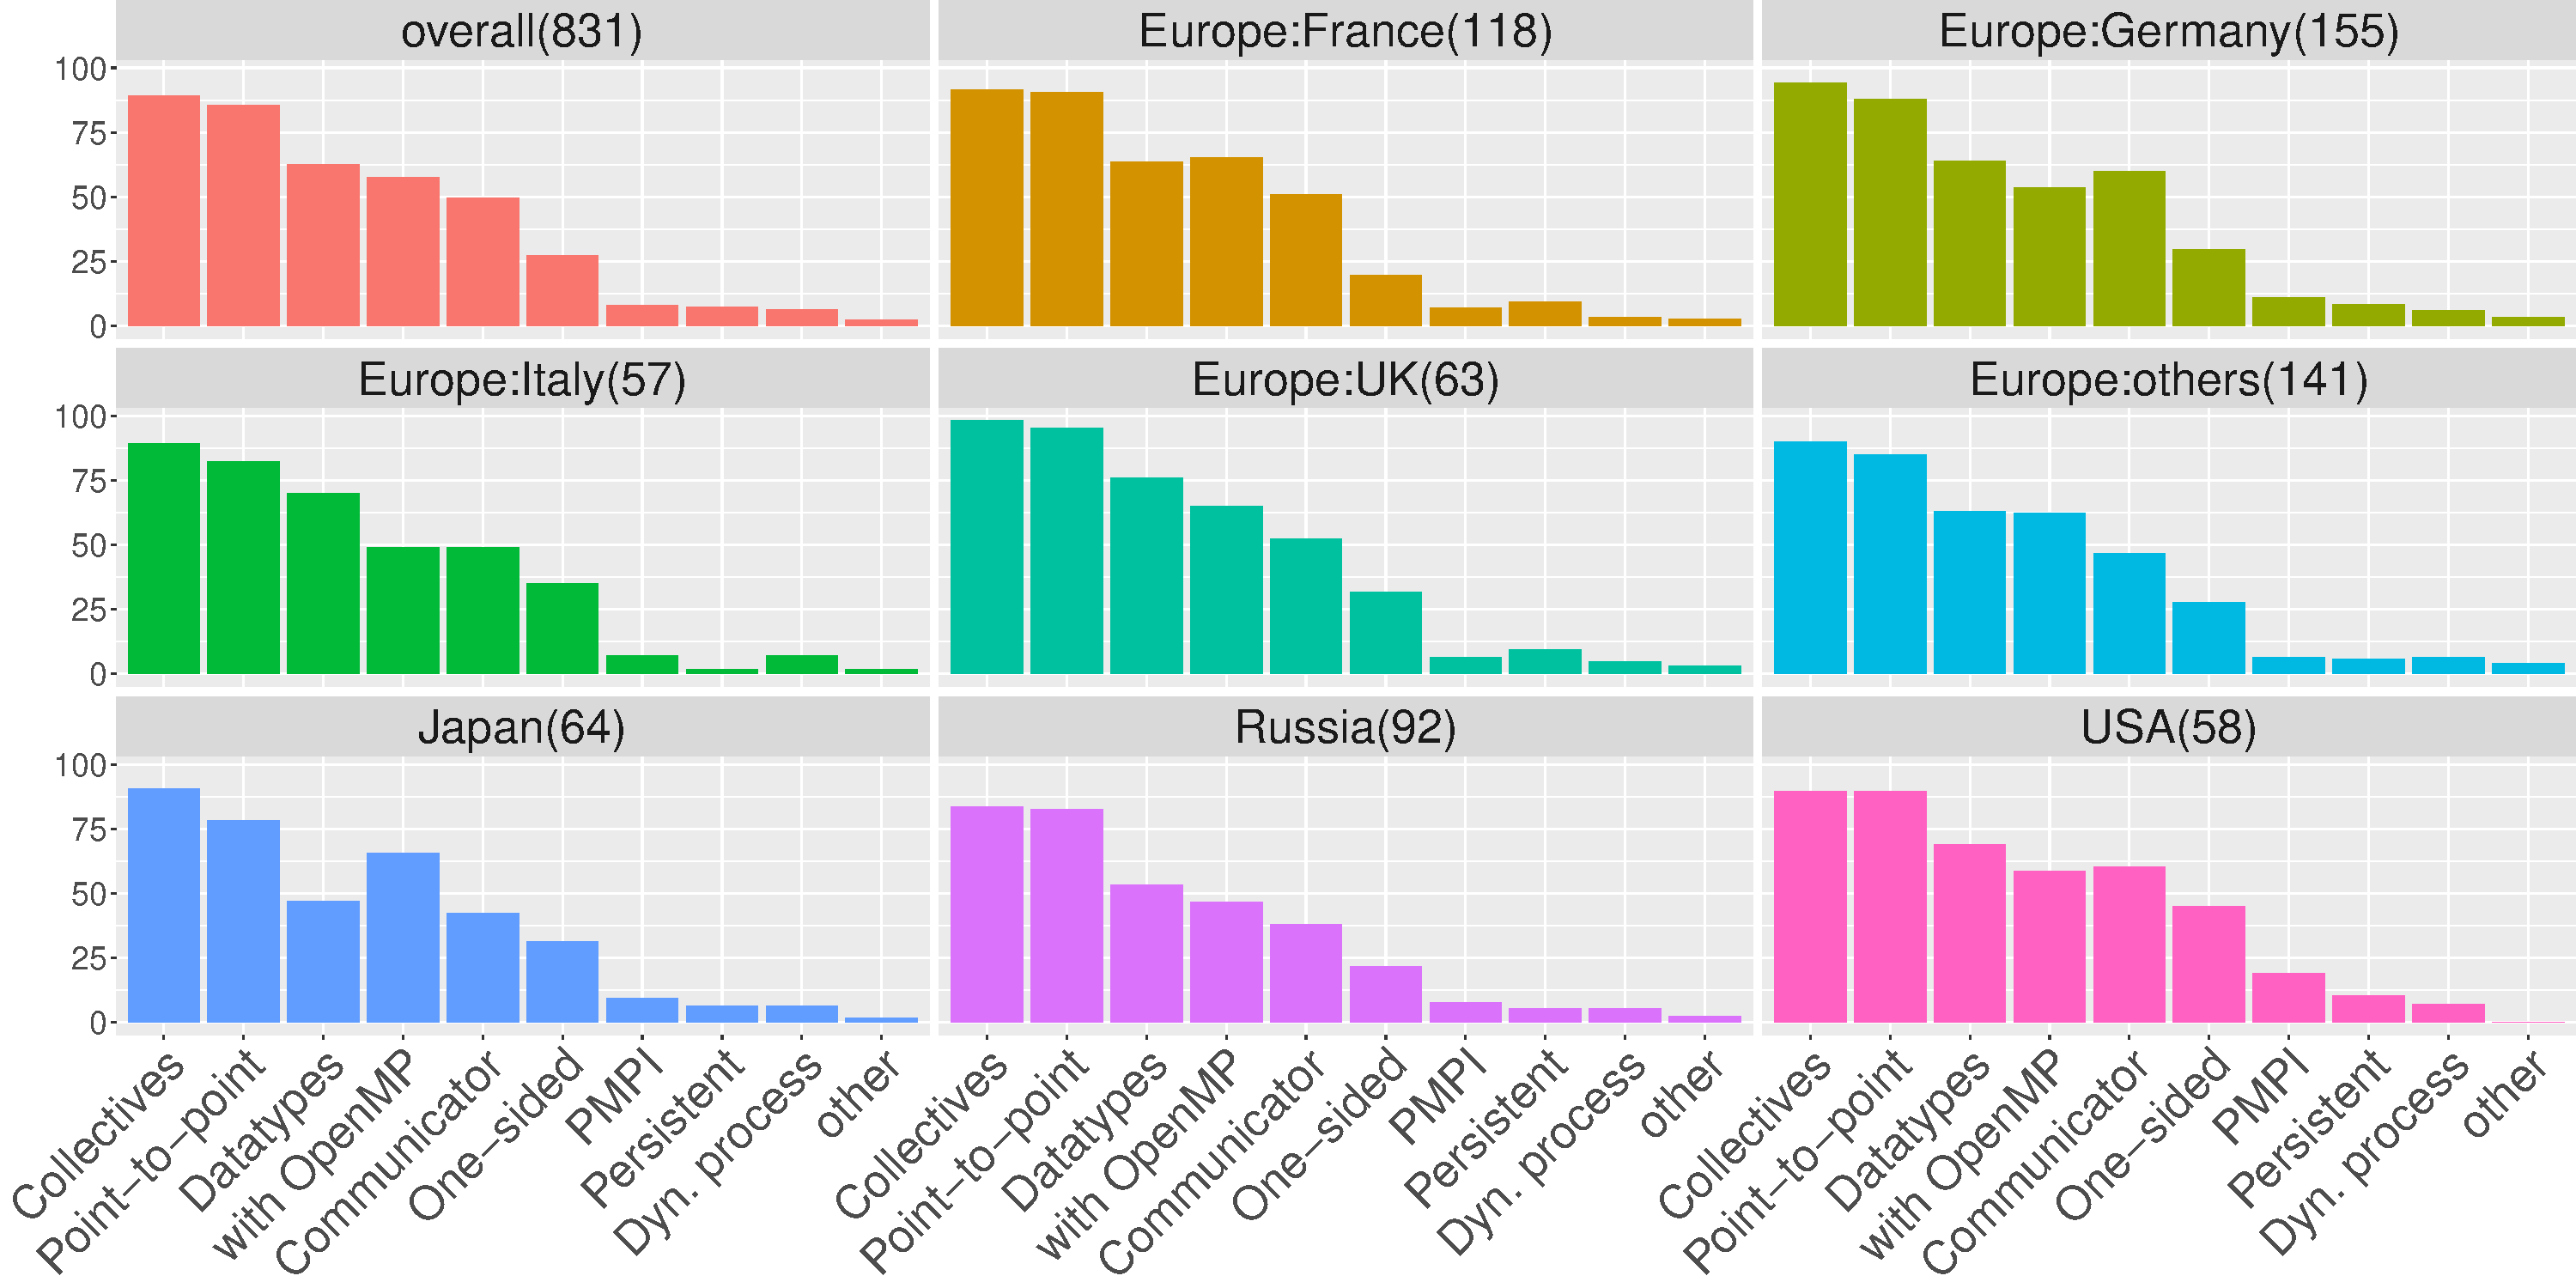
\includegraphics[width=8cm]{R-scripts/Q17.pdf}
    \caption{Q17: Using MPI Aspects {\it(multiple)}}
    \label{fig:using-mpi-aspects}
  \end{center}
\end{figure}

Most notable difference between our survey and the ECP survey is the
datatype (Table~\ref{tab:using-mpi-aspects}). The percentage in
datatype in ECP is 23\% and the percentage in our survey is more
than 60\% in both overall and USA. In the ECP survey, there are three
questions asking using MPI aspects in different usage scenarios; current,
exascale, and performance critical. In all three questions, the
percentages of using datatype are low.

\begin{table}[htb]%
  \begin{center}%
    \caption{Using MPI Aspects}\label{tab:using-mpi-aspects}%
    \begin{tabular}{c||c|c||c|c|c}%
      \hline%
      Choice & \multicolumn{2}{c||}{Our Survey [\%]} &
      \multicolumn{3}{c}{ECP [\%]} \\
      \cline{2-6}%
      & overall & USA & AD & ST & AD+ST \\
      \hline%
      Collectives & 89 & 90 & 86 & 75 & 80 \\
      Point-to-point & 85 & 90 & 96 & 79 & 88 \\
      Datatype & 63 & 69 & 25 & 21 & 23 \\
      Communicator & 50 & 60 & 68 & 54 & 61 \\
      One-sided (RMA) & 27 & 45 & 36 & 7 & 21 \\
      PMPI & 8 & 19 & 11 & 0 & 14 \\
      \hline%
    \end{tabular}%
  \end{center}%
\end{table}%

Fig.~\ref{fig:skill-and-aspects} is the addition. This graph is a
heatmap of the cross-tab analysis between Q3 asking MPI skill and Q16
asking unknown MPI features. The darker the color of a cell, the
higher the frequency (Legend combined with color bar can be found at
the bottom right. The numbers in the legend cells are
percentage). Less frequent 
rows (skill low (1) and skill high (6)) in this figure are
omitted. Natural thinking may conclude 
that the higher the MPI skill, lesser the unknown MPI features. The
result is quite interesting, the less used features in
Fig.~\ref{fig:using-mpi-aspects}, PMPI, persistent, and dynamic
process, are almost independent from the MPI skill. This may indicate
that the MPI standard is very profound. Even the most basic
send/receive functions, although they look very simple and natural,
they require deep knowledge such as possibility of deadlock, timing of
buffer access, blocking and non-blocking, and so on.

\begin{figure}[htb]
  \begin{center}
    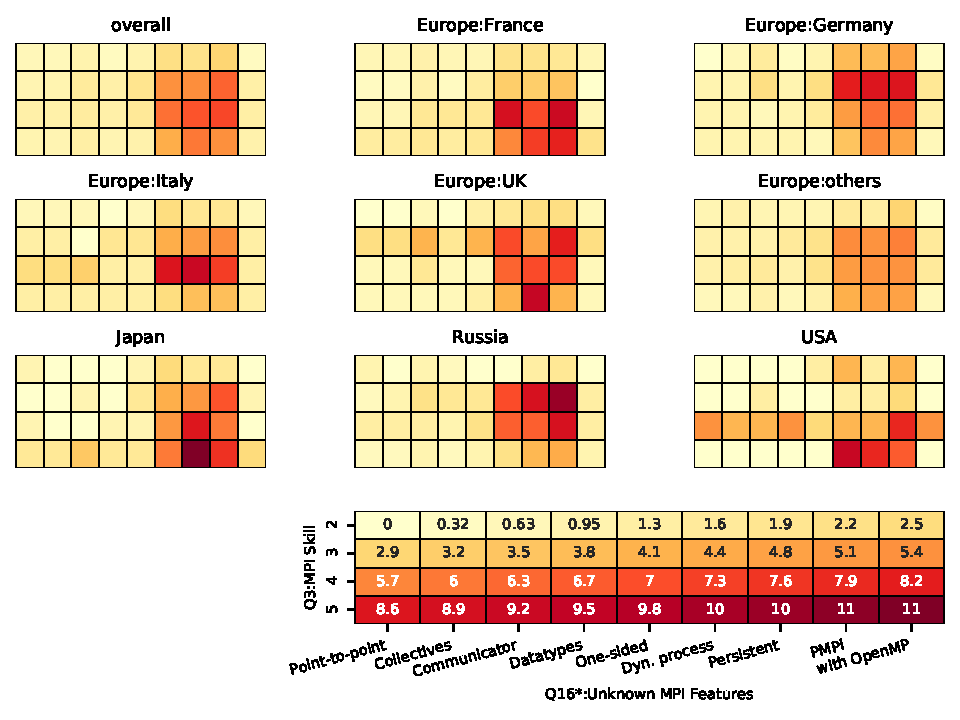
\includegraphics[width=8cm]{Figs/Q3-Q16.pdf}
    \caption{Q3-Q16: MPI Skill {\it(single)} and Unknown MPI Features {\it(multiple)}}
    \label{fig:skill-and-aspects}
  \end{center}
\end{figure}

Fig.~\ref{fig:useless-features} is the result of Q27 asking ``What MPI
feature(s) are NOT useful for your application?'' Although many
participants think MPI has no "not useful features", fairly amount of
participants think the dynamic process feature not useful. Thinking
of the fact that the dynamic process feature is not used by the most
participants (Q17, Fig.~\ref{fig:using-mpi-aspects}), this result is
quite interesting.
This tendency is also reported in \cite{10.1145/3295500.3356176}.

Fig.~\ref{fig:useless-features} is additionally shown here. The second
largest and considerable amount of percentage of the \myquote{dynamic
  process} answer to the question ``What MPI feature(s) are NOT useful
for your application?'' can be seen in this figure. This percentage
occupies about 60\% of the participants who answered they have
some useless features.

\begin{figure}[htb]
  \begin{center}
    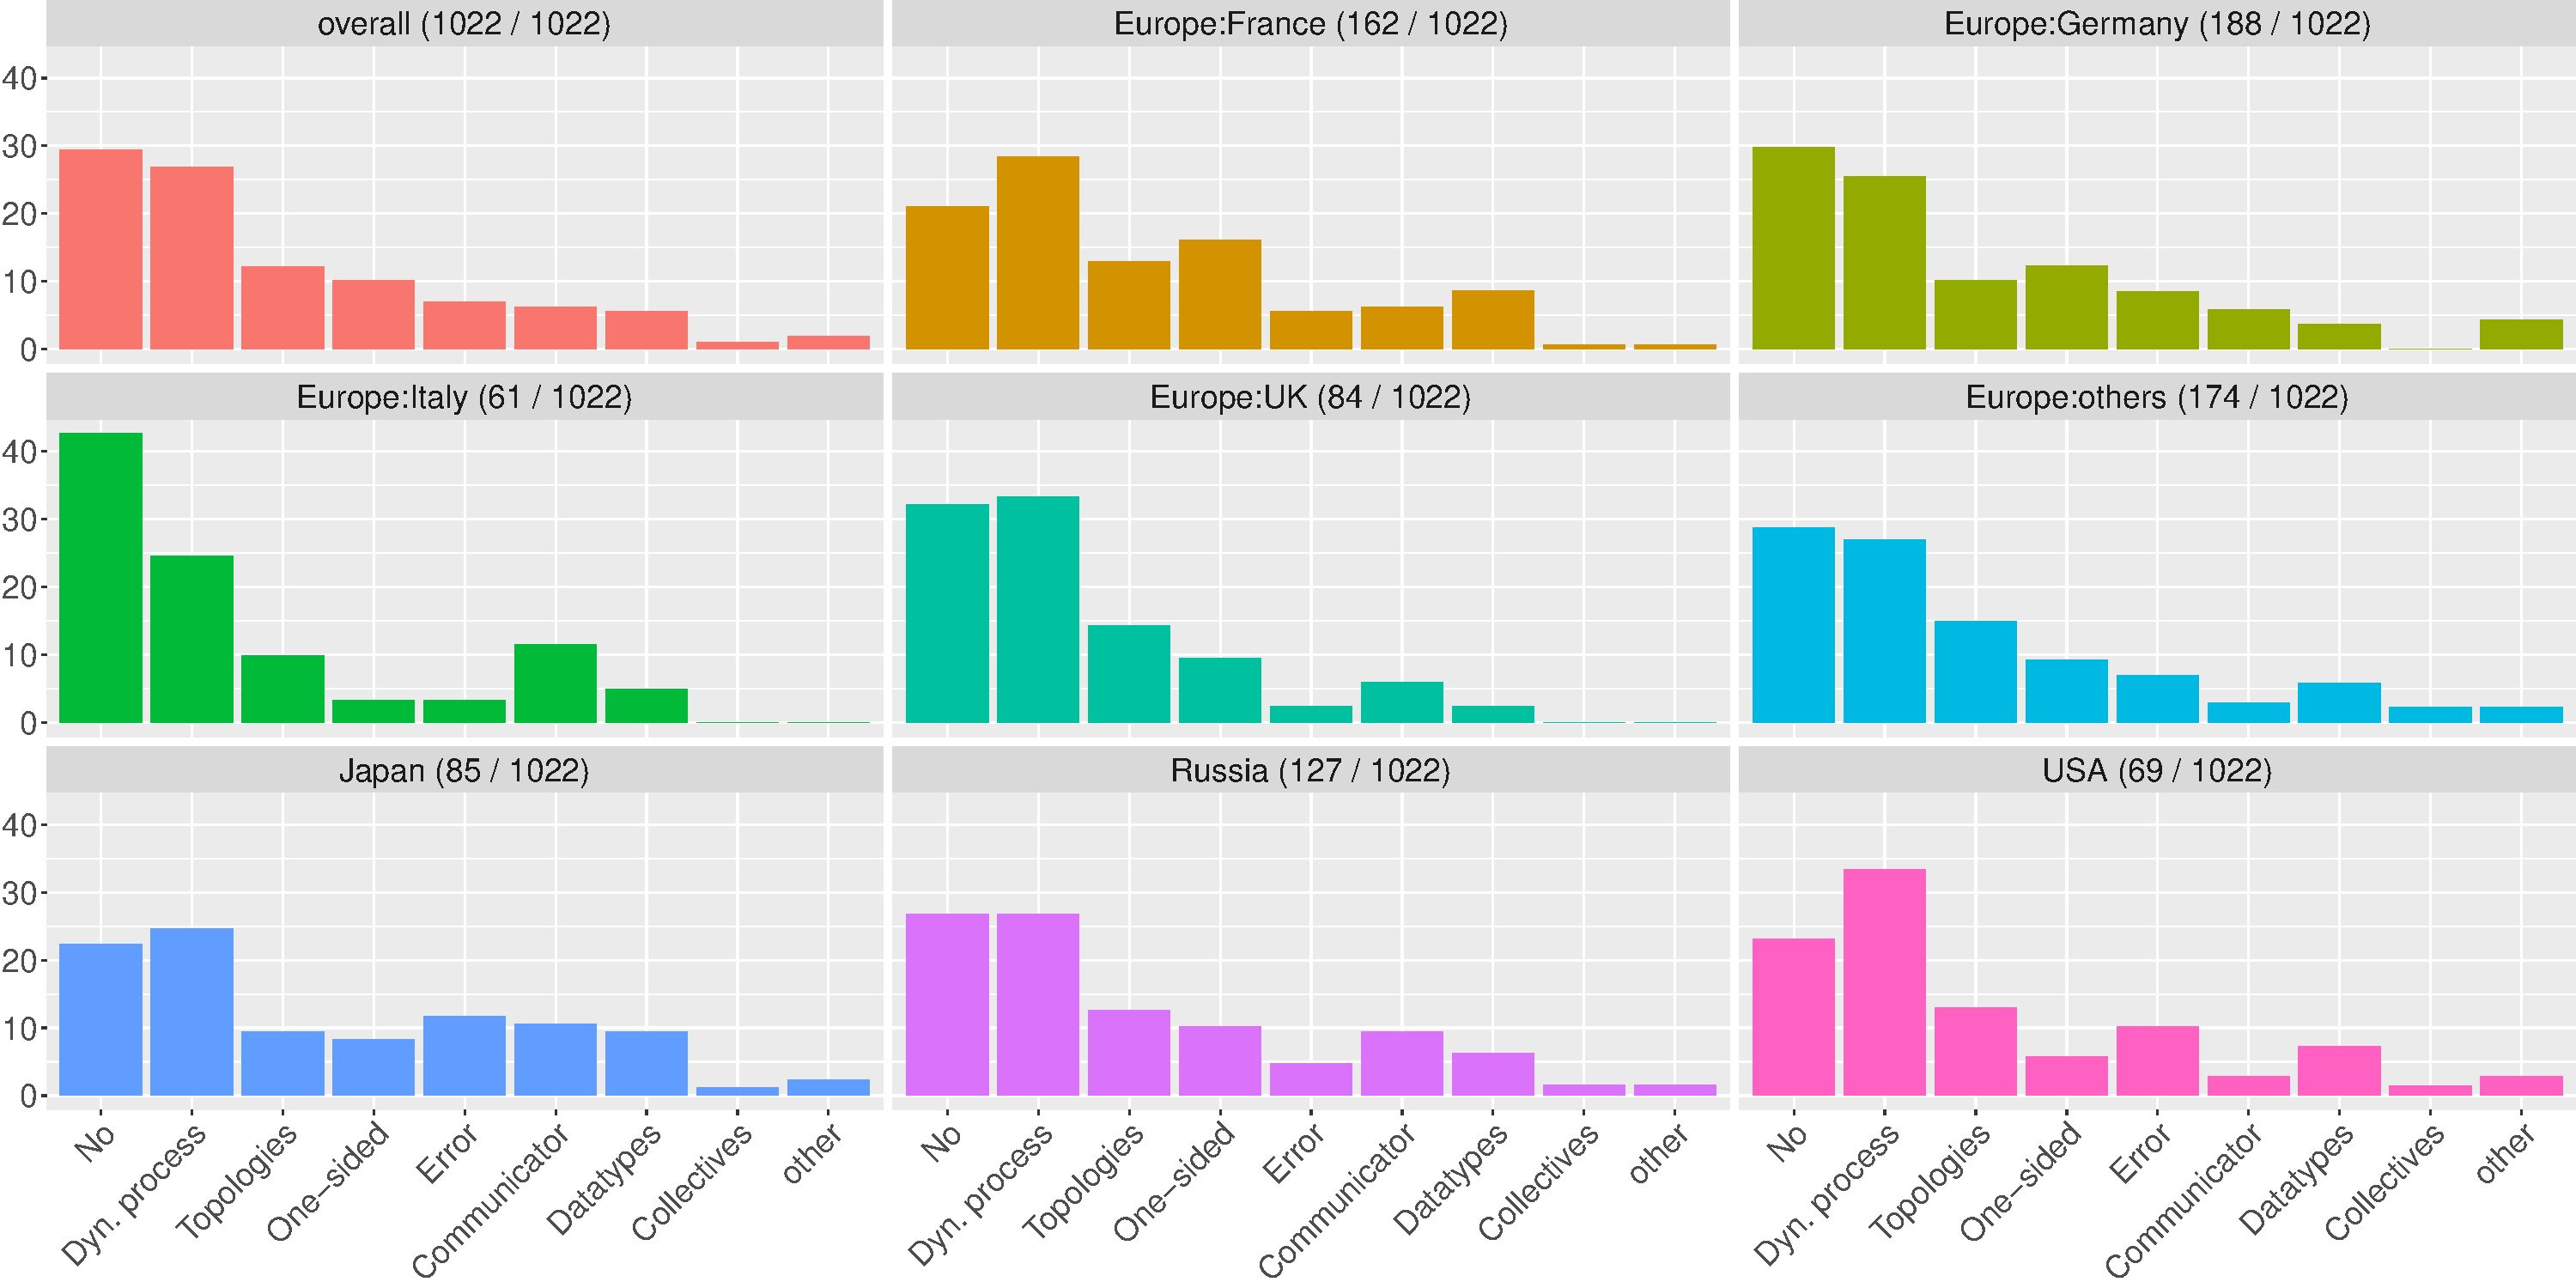
\includegraphics[width=8cm]{R-scripts/Q27.pdf}
    \caption{Q27: Useless Features {\it(multiple)}}
    \label{fig:useless-features}
  \end{center}
\end{figure}

The dynamic process feature is on the
border of process management and communication, since the process
creation itself is obviously out of the scope of the MPI standard,
while the communication between the existing (MPI) processes and newly
create (MPI) processes must be defined in the standard. Indeed, the
implementation of dynamic process creation spreads many parts of a
computing system: MPI library, process manager, job scheduling system
and system operation. This complexity might make the use of the
dynamic process creation hard and impractical for MPI users. 

\subsection{Multi-threading}

The difference between our survey and the ECP survey can be found on
the question asking multi-thread support. Fig.~\ref{fig:multi-thread}
shows the result of our survey and Table~\ref{tab:multi-thread} shows
the difference. Note that our question is multiple-answer and the ECP
question is single-answer. In both surveys (USA and ECP), the
percentage of using {\tt MULTIPLE} is the highest excepting the AD
case. However, the percentage of the choice \myquote{I don't know}
is fairly larger than ours. This may sound contradictory because the
ECP participants would be more experienced MPI users.

\begin{table}[htb]%
  \begin{center}%
    \caption{Multi-threading}\label{tab:multi-thread}%
    \begin{tabular}{c||c|c||c|c|c}%
      \hline%
      Choice & \multicolumn{2}{c||}{Our Survey [\%]} & 
      \multicolumn{3}{c}{ECP {\it(single)} [\%]} \\
      \cline{2-6}%
      & overall & USA & AD & ST & AD+ST \\
      \hline%
      SINGLE & 29 & 22 & \multicolumn{3}{c}{\tiny (no corresponding choice)} \\
      FUNNELED & 18 & 13 & 18 & 18 & 18 \\
      SERIALIZED & 12 & 10 & 18 & 18 & 18 \\
      MULTIPLE & 22 & 31 & 18 & 32 & 25 \\
      never used & 23 & 16 & \multicolumn{3}{c}{\tiny (no corresponding choice)} \\
      not know & 14 & 8 & 25 & 25 & 25\\
      \hline%
    \end{tabular}%
  \end{center}%
\end{table}%

The usage of {\tt MULTIPLE} in US is also the highest among the major
regions (Fig.~\ref{fig:multi-thread}). France and Germany have the
same trend. In Italy, Japan, Russia and the
other countries in Europe, the percentages of \myquote{I don't know}
are the highest. In UK, the percentage of using {\tt SINGLE} is the
highest.

\begin{figure}[htb]
  \begin{center}
    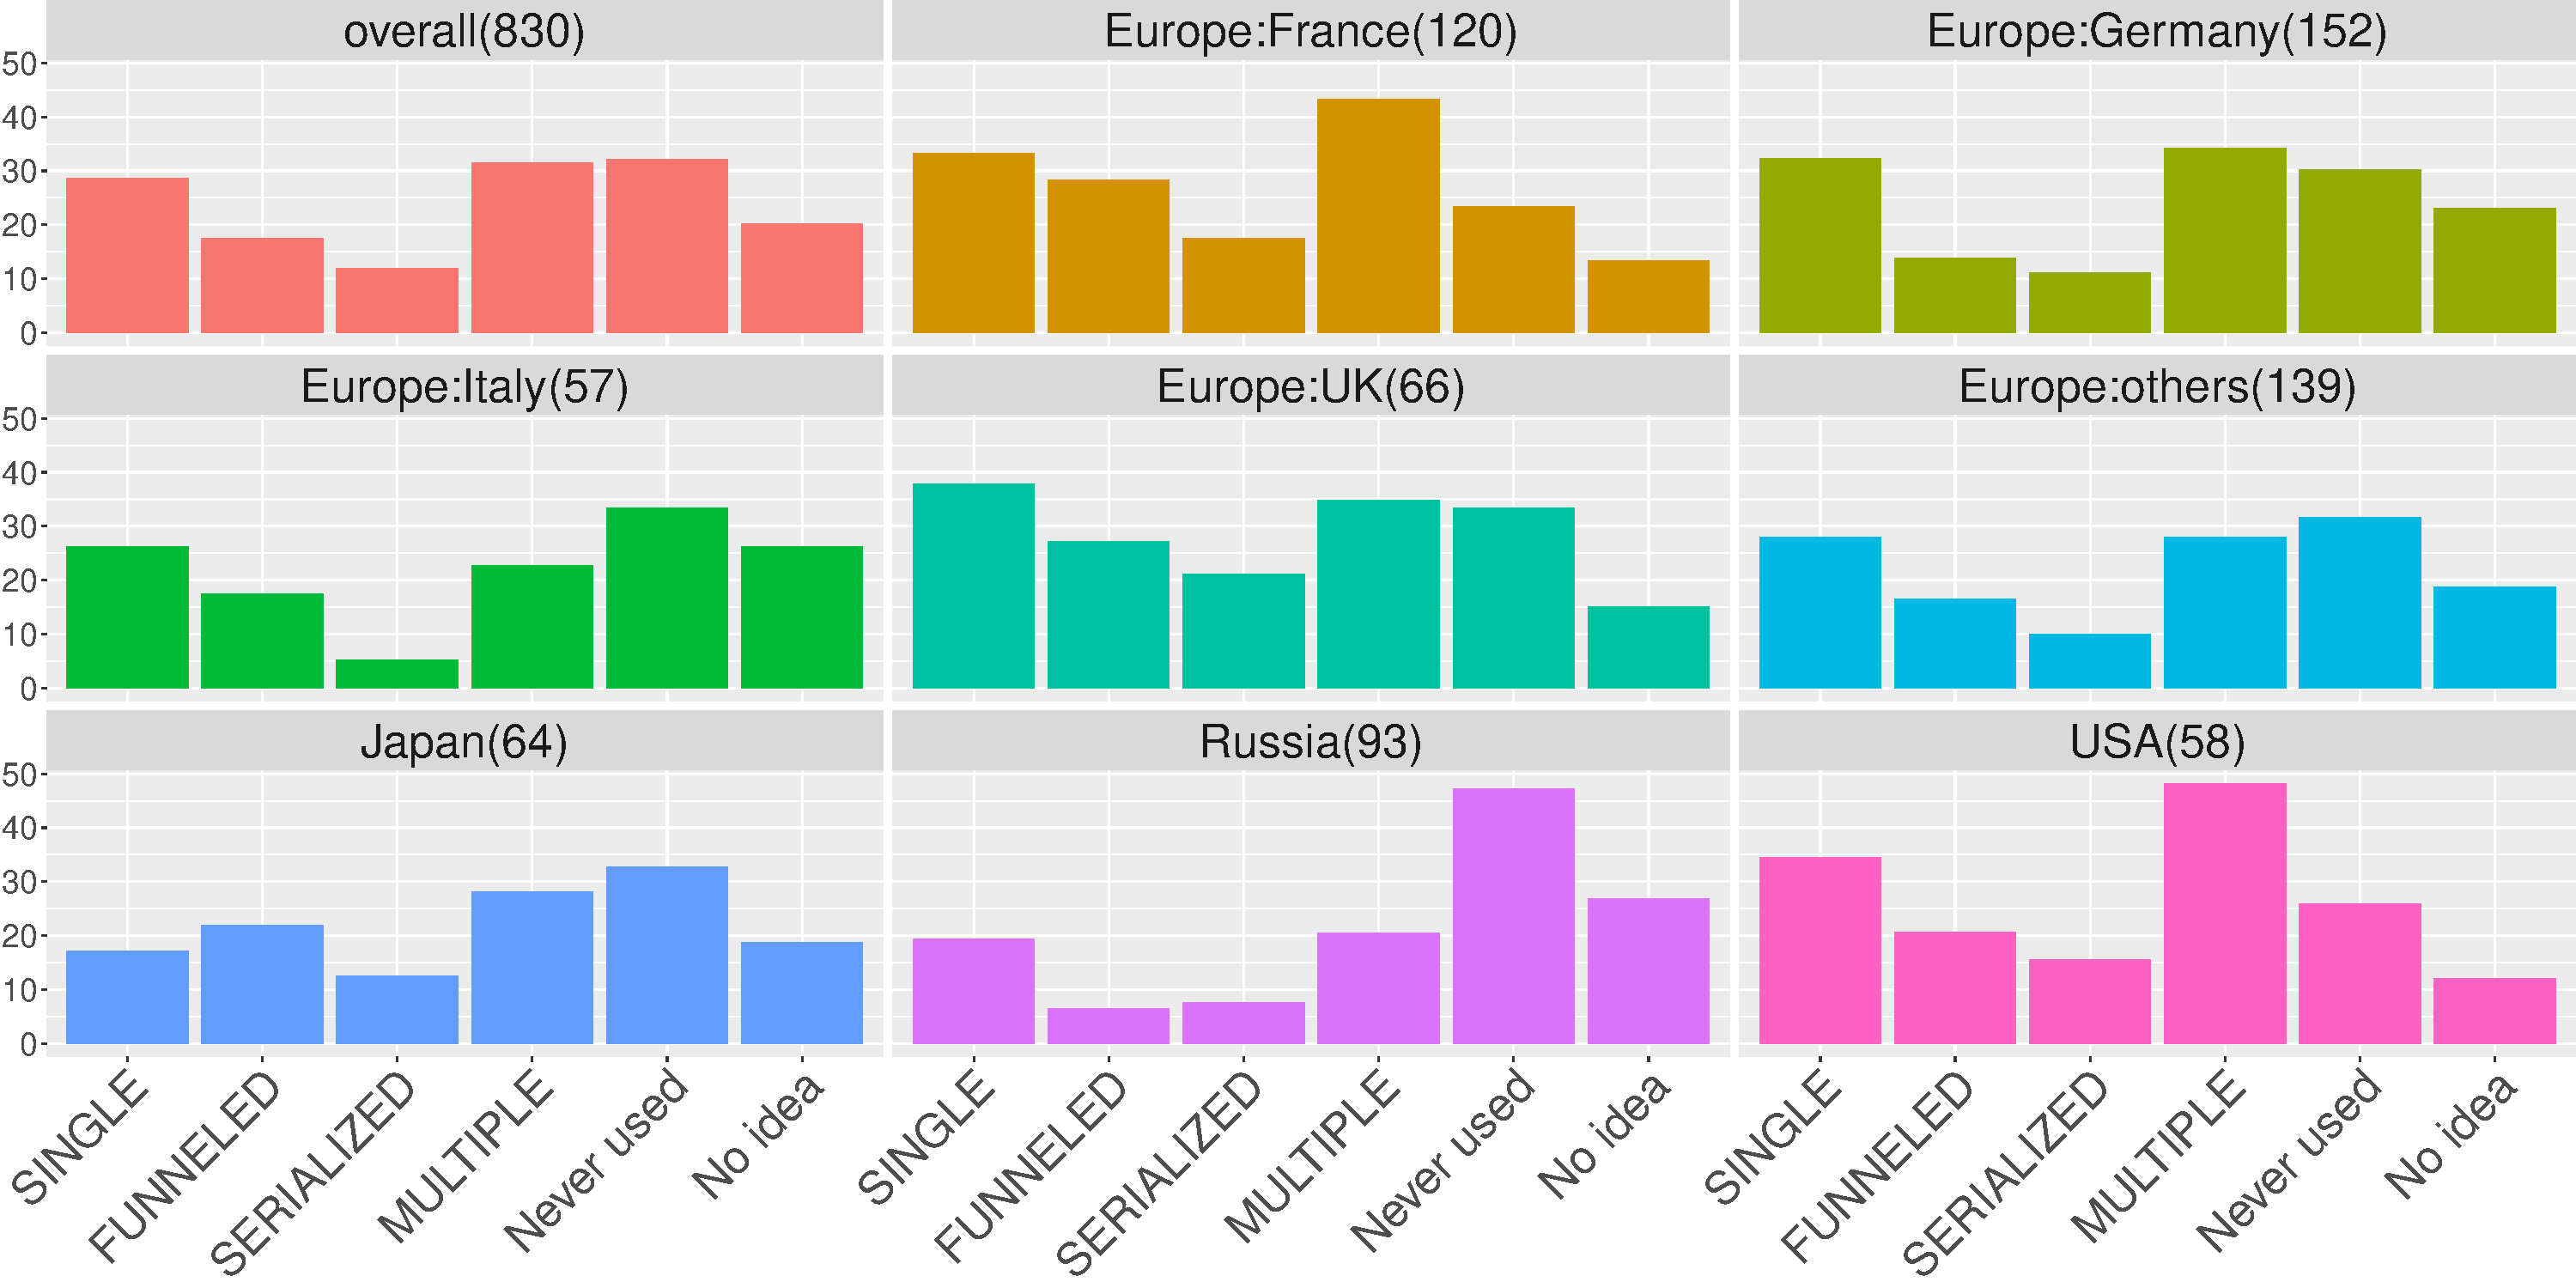
\includegraphics[width=8cm]{R-scripts/Q18.pdf}
    \caption{Q18: Multi-threading {\it(multiple)}}
    \label{fig:multi-thread}
  \end{center}
\end{figure}

Remember this is a multiple answer
question. Table~\ref{tab:multi-thread-raw} shows the top 7 of the 
percentages of raw answers (combined answers) of the
overall. These top 7 percentages occupy about 85\% in
total. Nearly half 
participants answered \myquote{never used} or \myquote{no idea.} The
numbers in parenthesis in this table are the percentage of 
participants excluding those who answered \myquote{never used} or
\myquote{no idea.} Half of threading-aware participants are using {\tt
  SINGLE}
and/or {\tt MULTIPLE}. Although many participants ignore the thread
mode, however, some participants use a particular thread support ({\tt
  SINGLE} or {\tt MULTIPLE}) and some other participants select one of
supported thread capabilities positively. 

\begin{table}[htb]%
  \begin{center}%
    \caption{Multi-threading - Raw Answers}\label{tab:multi-thread-raw}%
    \begin{tabular}{c|c}%
      \hline%
      Threading Support & Overall \\
      & Percentage \\
      \hline%
      \myquote{never used} + \myquote{no idea} & 48 \\
              {\tt MULTIPLE} & 12 (23) \\
              {\tt SINGLE, MULTIPLE} & 8 (16) \\
              {\tt SINGLE} & 7 (14) \\
              {\tt SINGLE, FUNNELED, SERIALIZED, MULTIPLE} & 4 (8) \\
              {\tt SINGLE, FUNNELED} & 3 (7) \\
              {\tt SERIALIZED} & 3 (5) \\
              \hline%
              \multicolumn{2}{c}{\footnotesize Numbers in parenthesis are
                percentages excluding \myquote{never used} and \myquote{no
                  ides}} 
    \end{tabular}%
  \end{center}%
\end{table}%

In~\cite{10.1109/SC.2018.00033}, approximately 75\% of their target
executables (not number of jobs) on Mira (total of 68) are using {\tt
  SINGLE}, 15\% use {\tt FUNNELED} and 4\% use {\tt
  MULTIPLE}. In \cite{10.1145/3295500.3356176},  approximately 60\% of
their target programs use {\tt FUNNELED}, 30\% use {\tt MULTIPLE}, 20\%
use {\tt SINGLE} and only few percent use {\tt SERIALIZED}. Thus, the
thread support usage varies on each survey and further investigation
is needed to state a result.

\section{Other Findings}

\comment{
  \subsection{MPI Implementations}

  Fig.~\ref{fig:using-implementations} shows the Q12 result. The top 3
  implementations, Open MPI, Intel MPI and MPICH, dominates in all
  countries and regions, followed by MVAPICH. A large disparity can be
  seen on the other implementations. Taking a
  look at the \myquote{other} choice, there are four (4) answers raising the
  \myquote{bullx MPI} and another four (4) using MadMPI~\cite{madmpi} in
  France, and 10 
  answers raising ParaStation MPI in Germany. The frequency of using
  Fujitsu MPI, ParaStation MPI, bullx MPI and others heavily depend on
  countries of participants and the countries where the MPI was
  developed. 

  \begin{figure}[htb]
    \begin{center}
      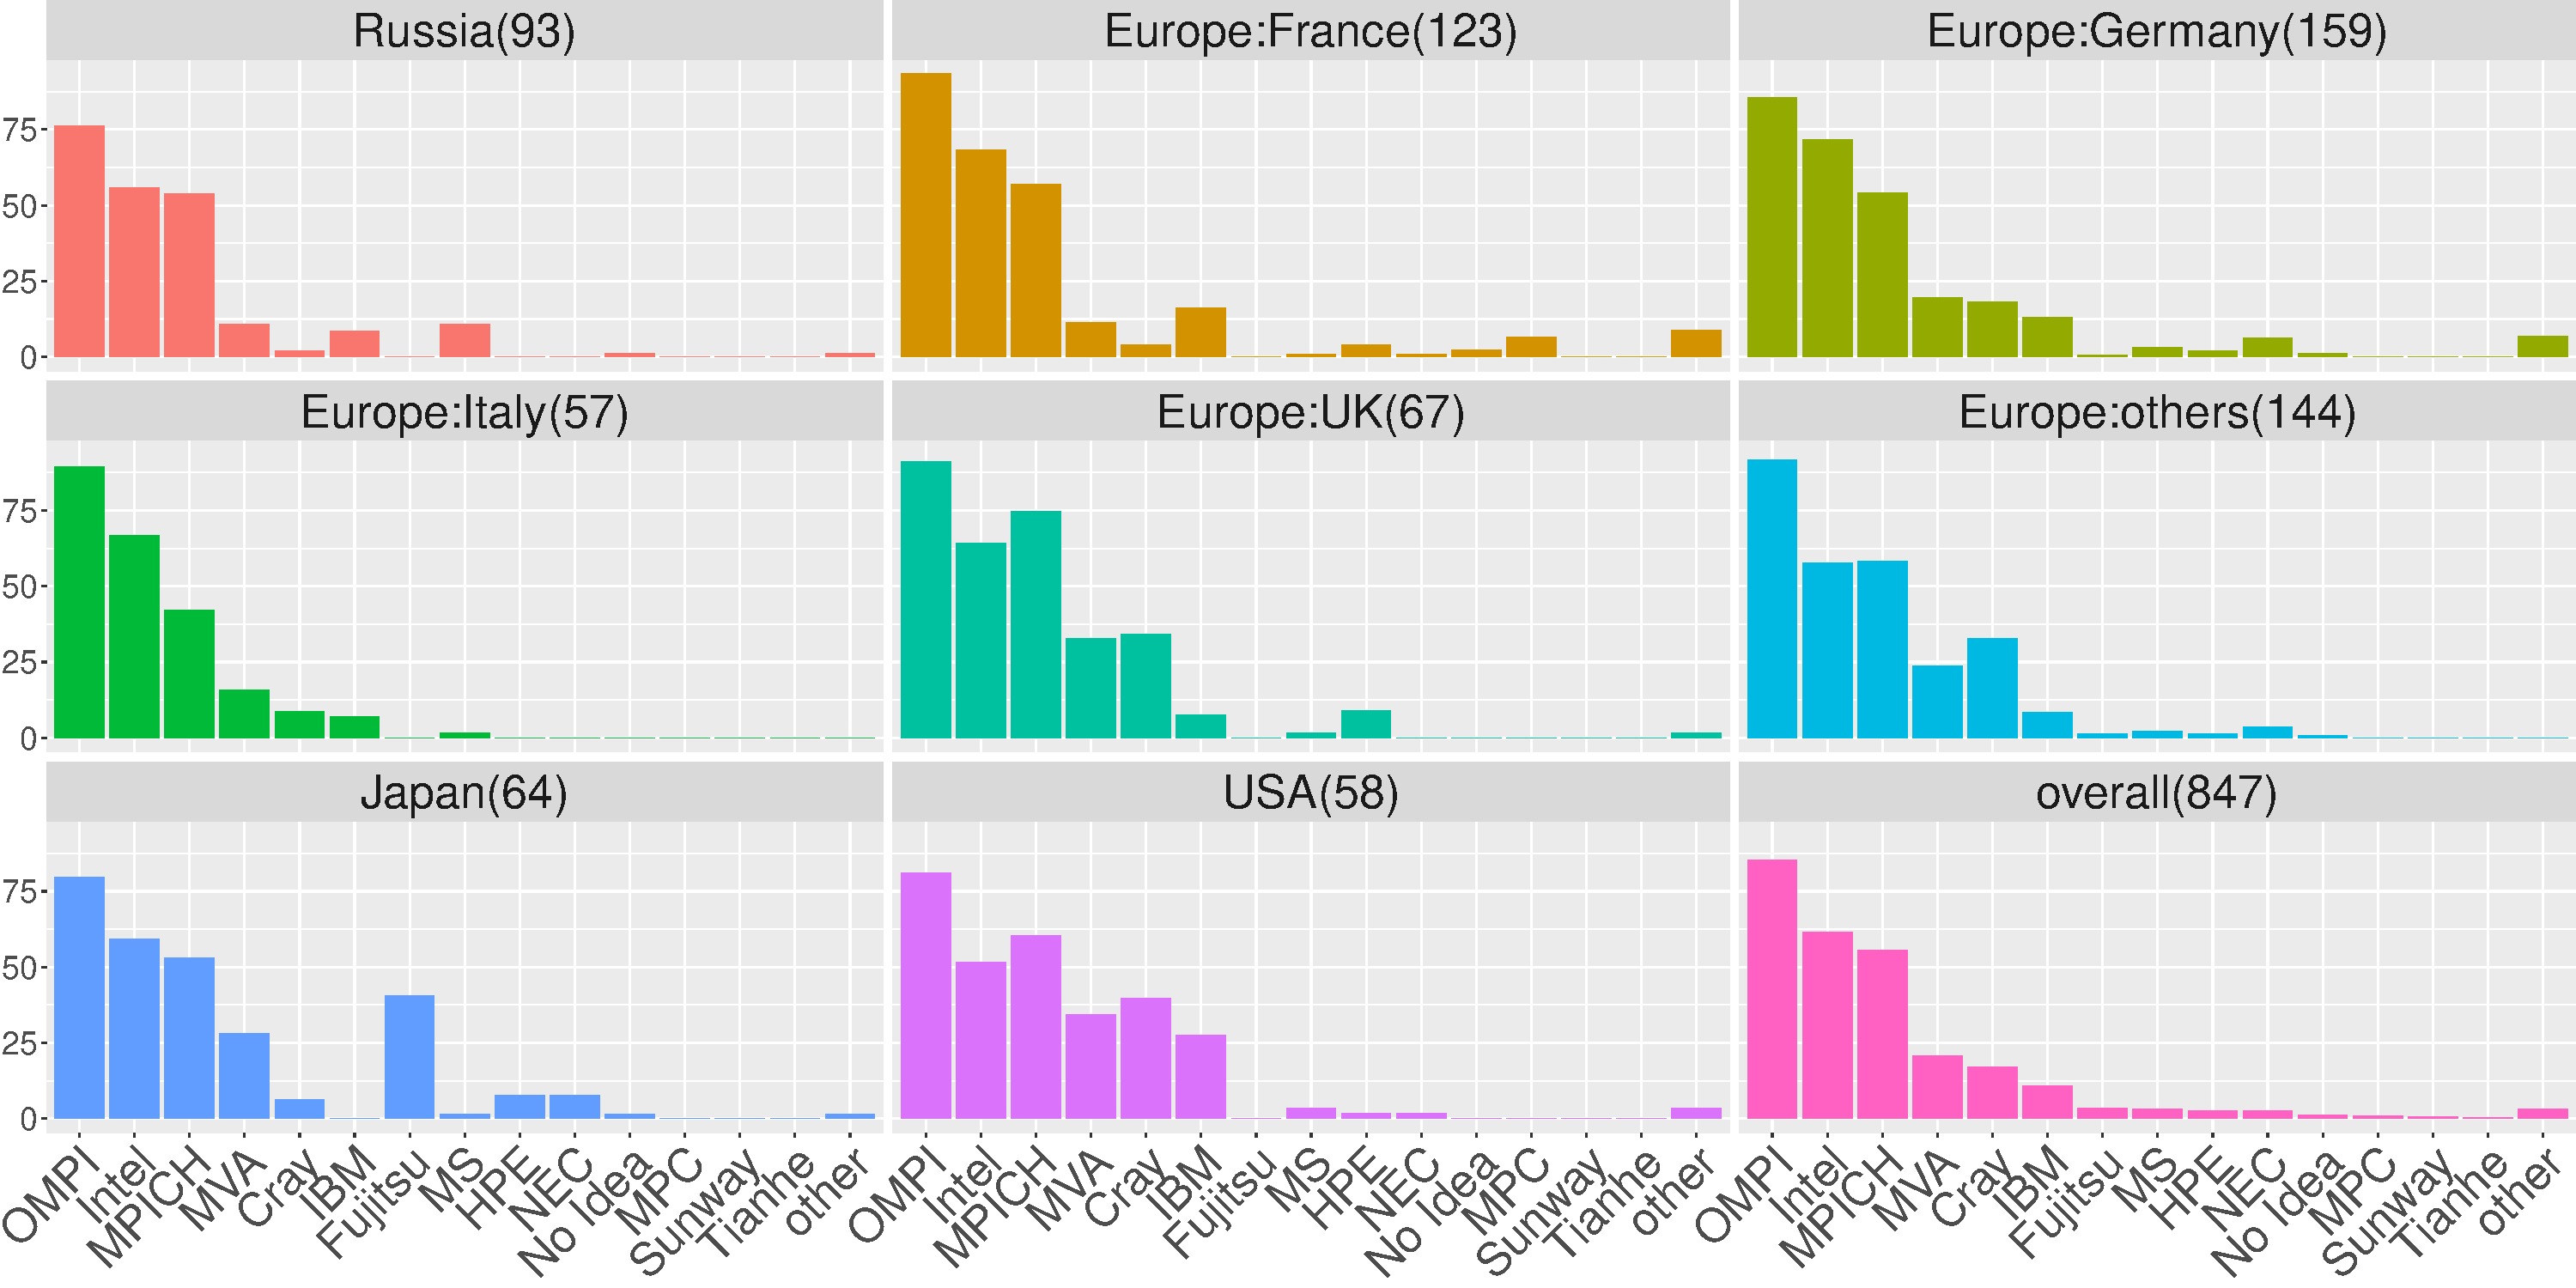
\includegraphics[width=8cm]{R-scripts/Q12.pdf}
      \caption{Q12: Using MPI Implementations {\it(multiple)}}
      \label{fig:using-implementations}
    \end{center}
  \end{figure}

  \comment{
    Q13 is asking ``why did you choose the MPI implementation(s)'' and its
    answers are shown in Fig.~\ref{fig:choosing-implementation}. The highest
    percentage of US participants selected `Familiar.' Many Italian
    participants also selected \myquote{Familiar.} Many Russian
    participants selected \myquote{No reason.} The largest part of UK and Germany
    participants selected \myquote{No choice.}
    In general, more than half of participants excepting US select MPI
    implementation(s) without any reason nor freedom of choice.
    
    \begin{figure}[htb]
      \begin{center}
        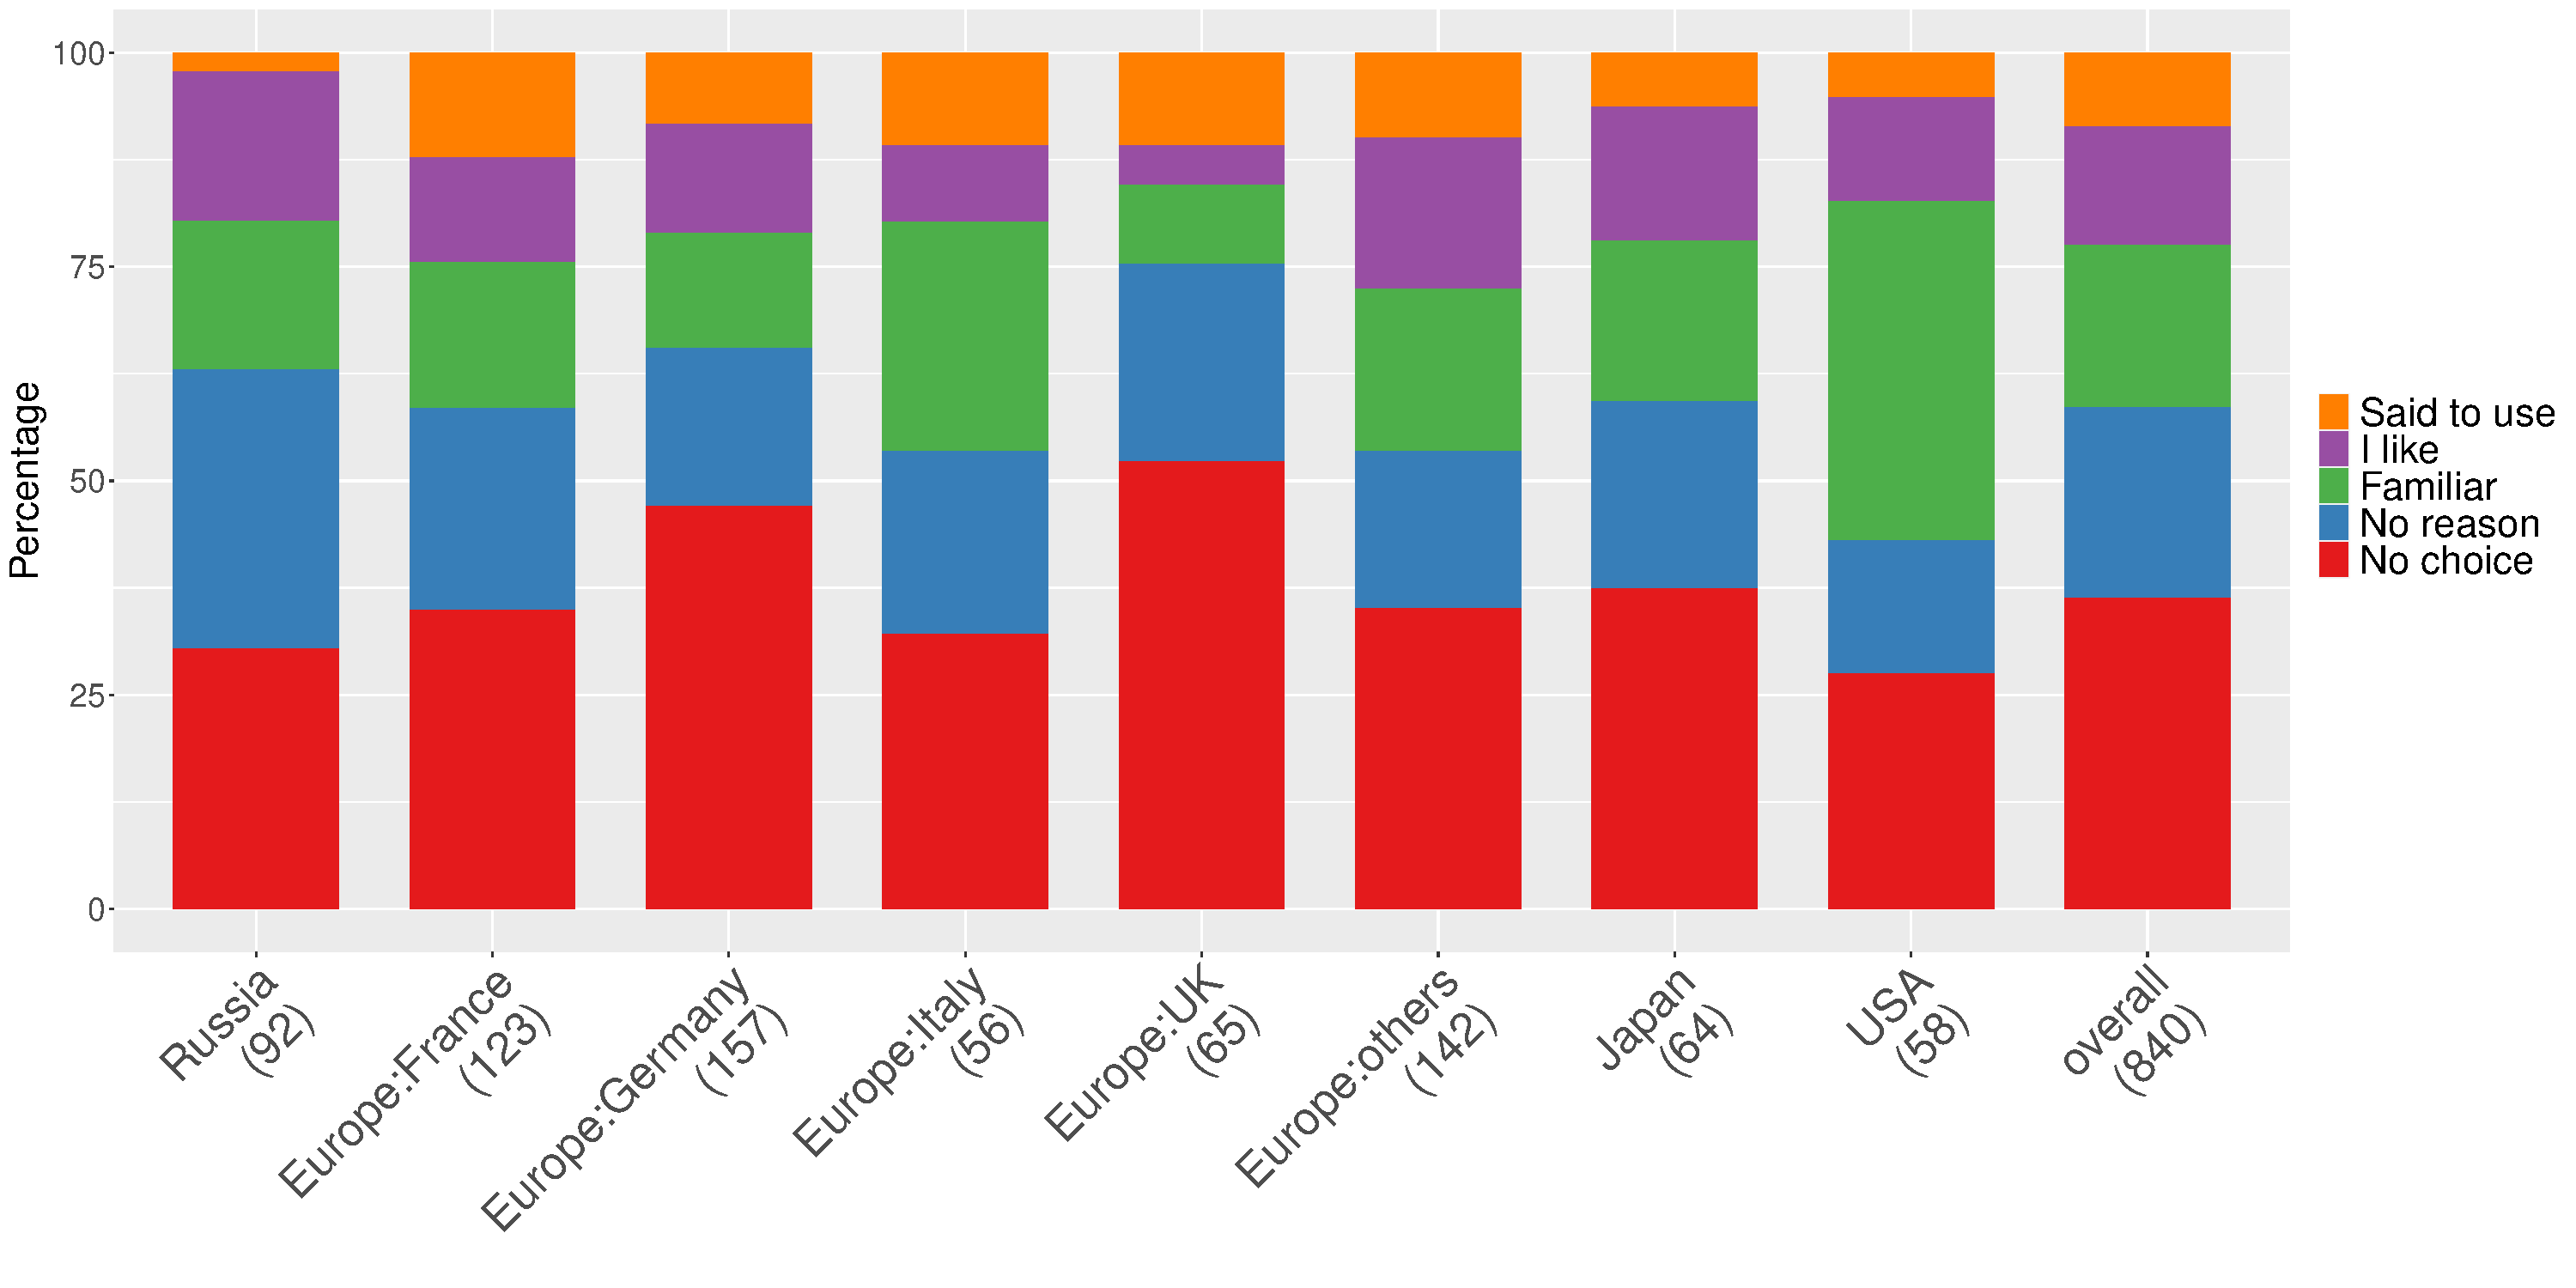
\includegraphics[width=9cm]{R-scripts/Q13.pdf}
        \caption{Q13: Choosing MPI Implementations {\it(single)}}
        \label{fig:choosing-implementation}
      \end{center}
    \end{figure}
  }
}
        
\subsection{Learning MPI}

Fig.~\ref{fig:learning-mpi} shows the percentages of how participants
learned MPI. In this graph, \myquote{Other lec.} indicates the choice
\myquote{Other lectures or tutorials (workplace, conference)}. The
UK and Russia participants preferred to learn by Internet. The
participants of Germany and other European countries preferred to have
other lectures. The percentage of reading \myquote{Books} in US is the
highest. Taking a look at the other answers, 18 participants learned
by reading existing code and 8 participants learned by
doing\footnote{One participant answered \myquote{reverse engineering!}}. 

\begin{figure}[htb]
\begin{center}
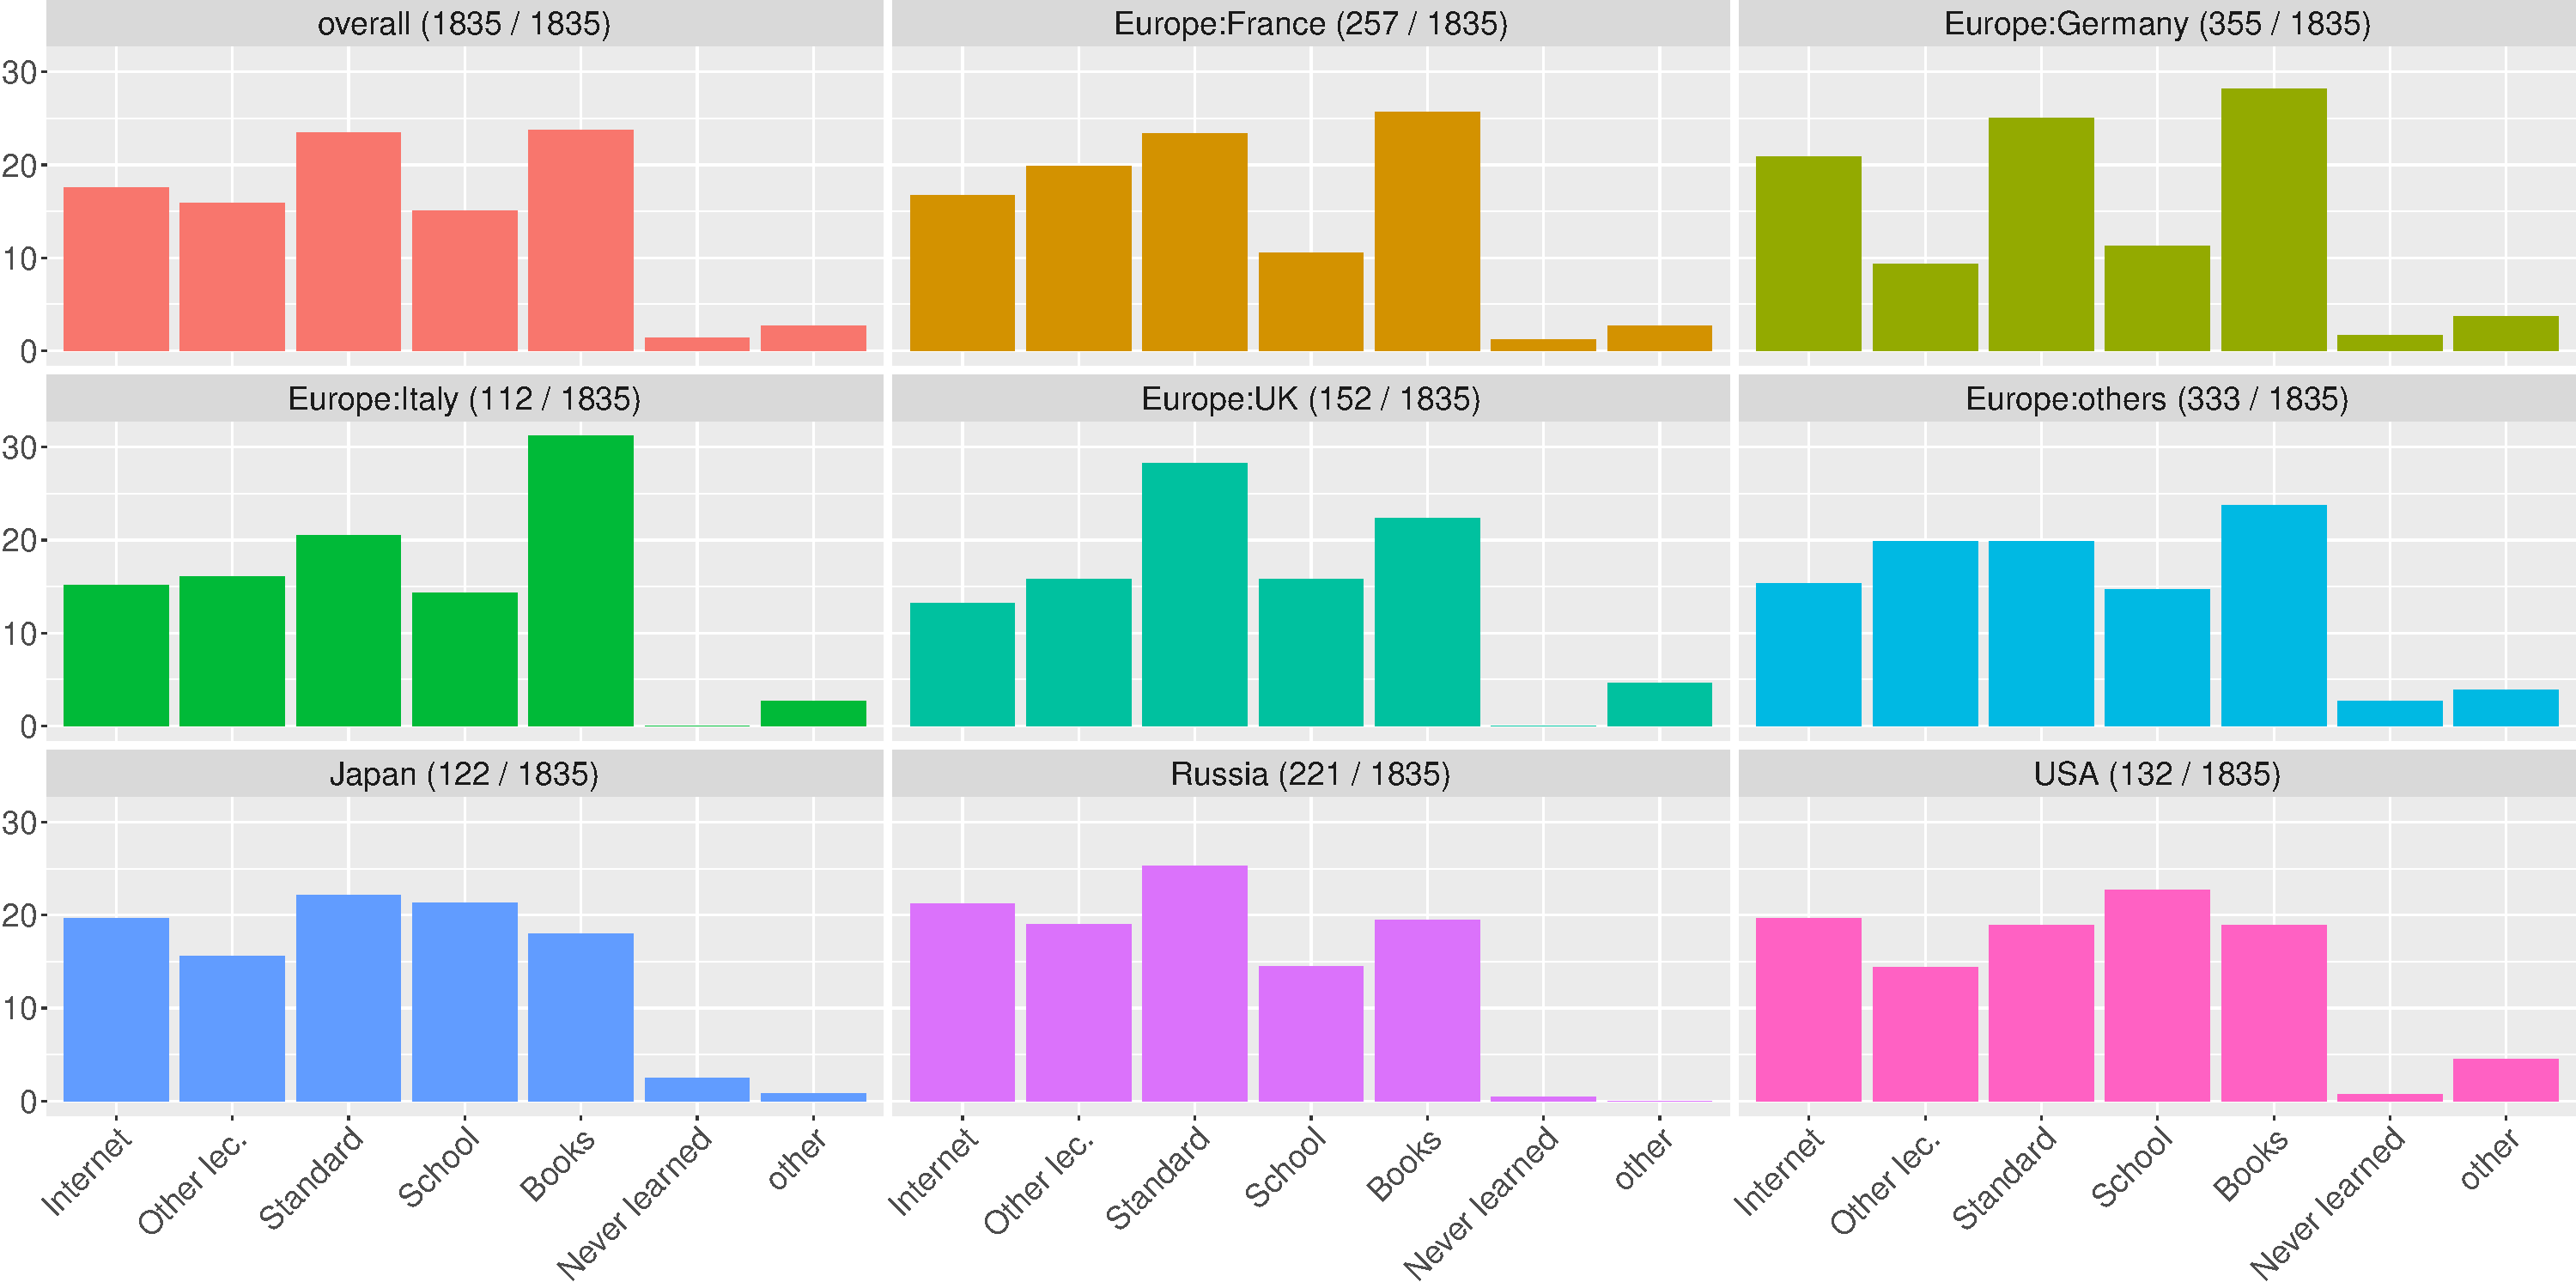
\includegraphics[width=8cm]{R-scripts/Q10.pdf}
\caption{Q10: Learning MPI {\it(multiple)}}
\label{fig:learning-mpi}
\end{center}
\end{figure}

Fig.~\ref{fig:reading-standard} shows the graph of Q9, asking if
participants have read the MPI standard document. Not surprisingly,
around 60\% of participants, independent from countries, read the
standard partly. Most interesting country is UK, where the percentage
of participants reading all document and, at the same time, the
percentage of the answer \myquote{No, and I will not read it} are the
highest among the countries and regions. 

\begin{figure}[htb]
\begin{center}
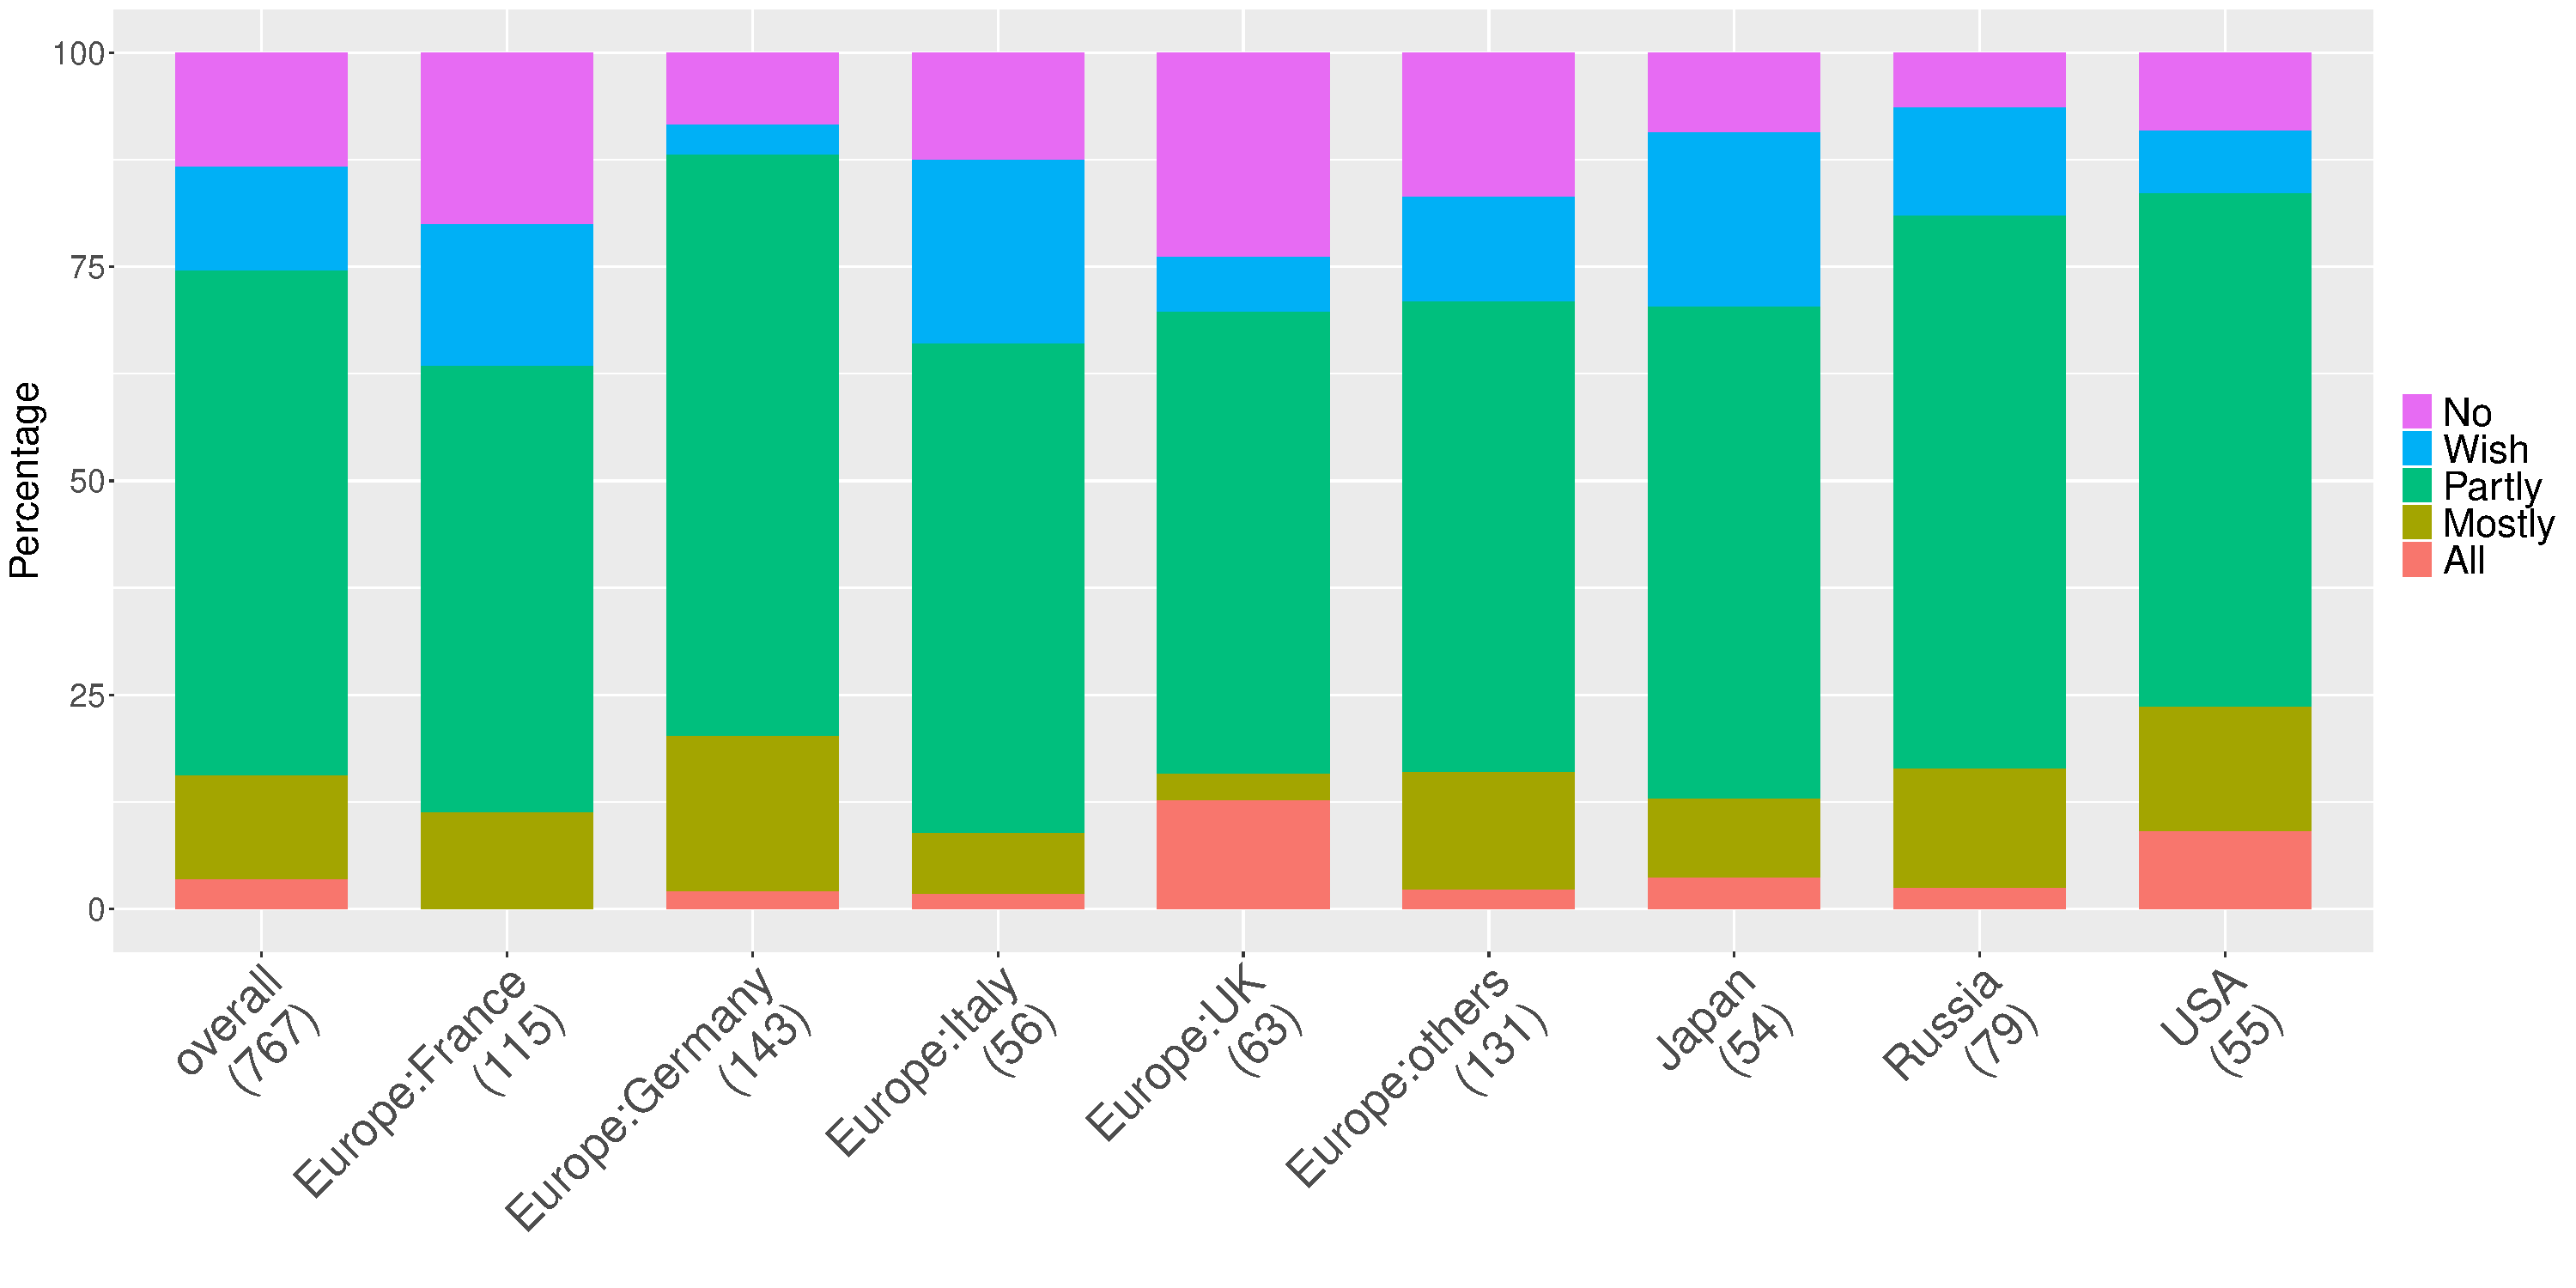
\includegraphics[width=9cm]{R-scripts/Q9.pdf}
\caption{Q9: Reading MPI Standard {\it(single)}}
\label{fig:reading-standard}
\end{center}
\end{figure}

Now let's see how people are writing MPI
programs. Fig.~\ref{fig:checking-spec} shows the percentages of Q14
asking ``How do you check MPI specifications when your are writing MPI
programs?'' Most users are checking MPI specifications by reading online
documentations (e.g., man pages), searching Internet and reading the
standard. As shown in the previous figure
(Fig.~\ref{fig:reading-standard}), users are reading the standard
partly because of checking the MPI specifications.

\begin{figure}[htb]
\begin{center}
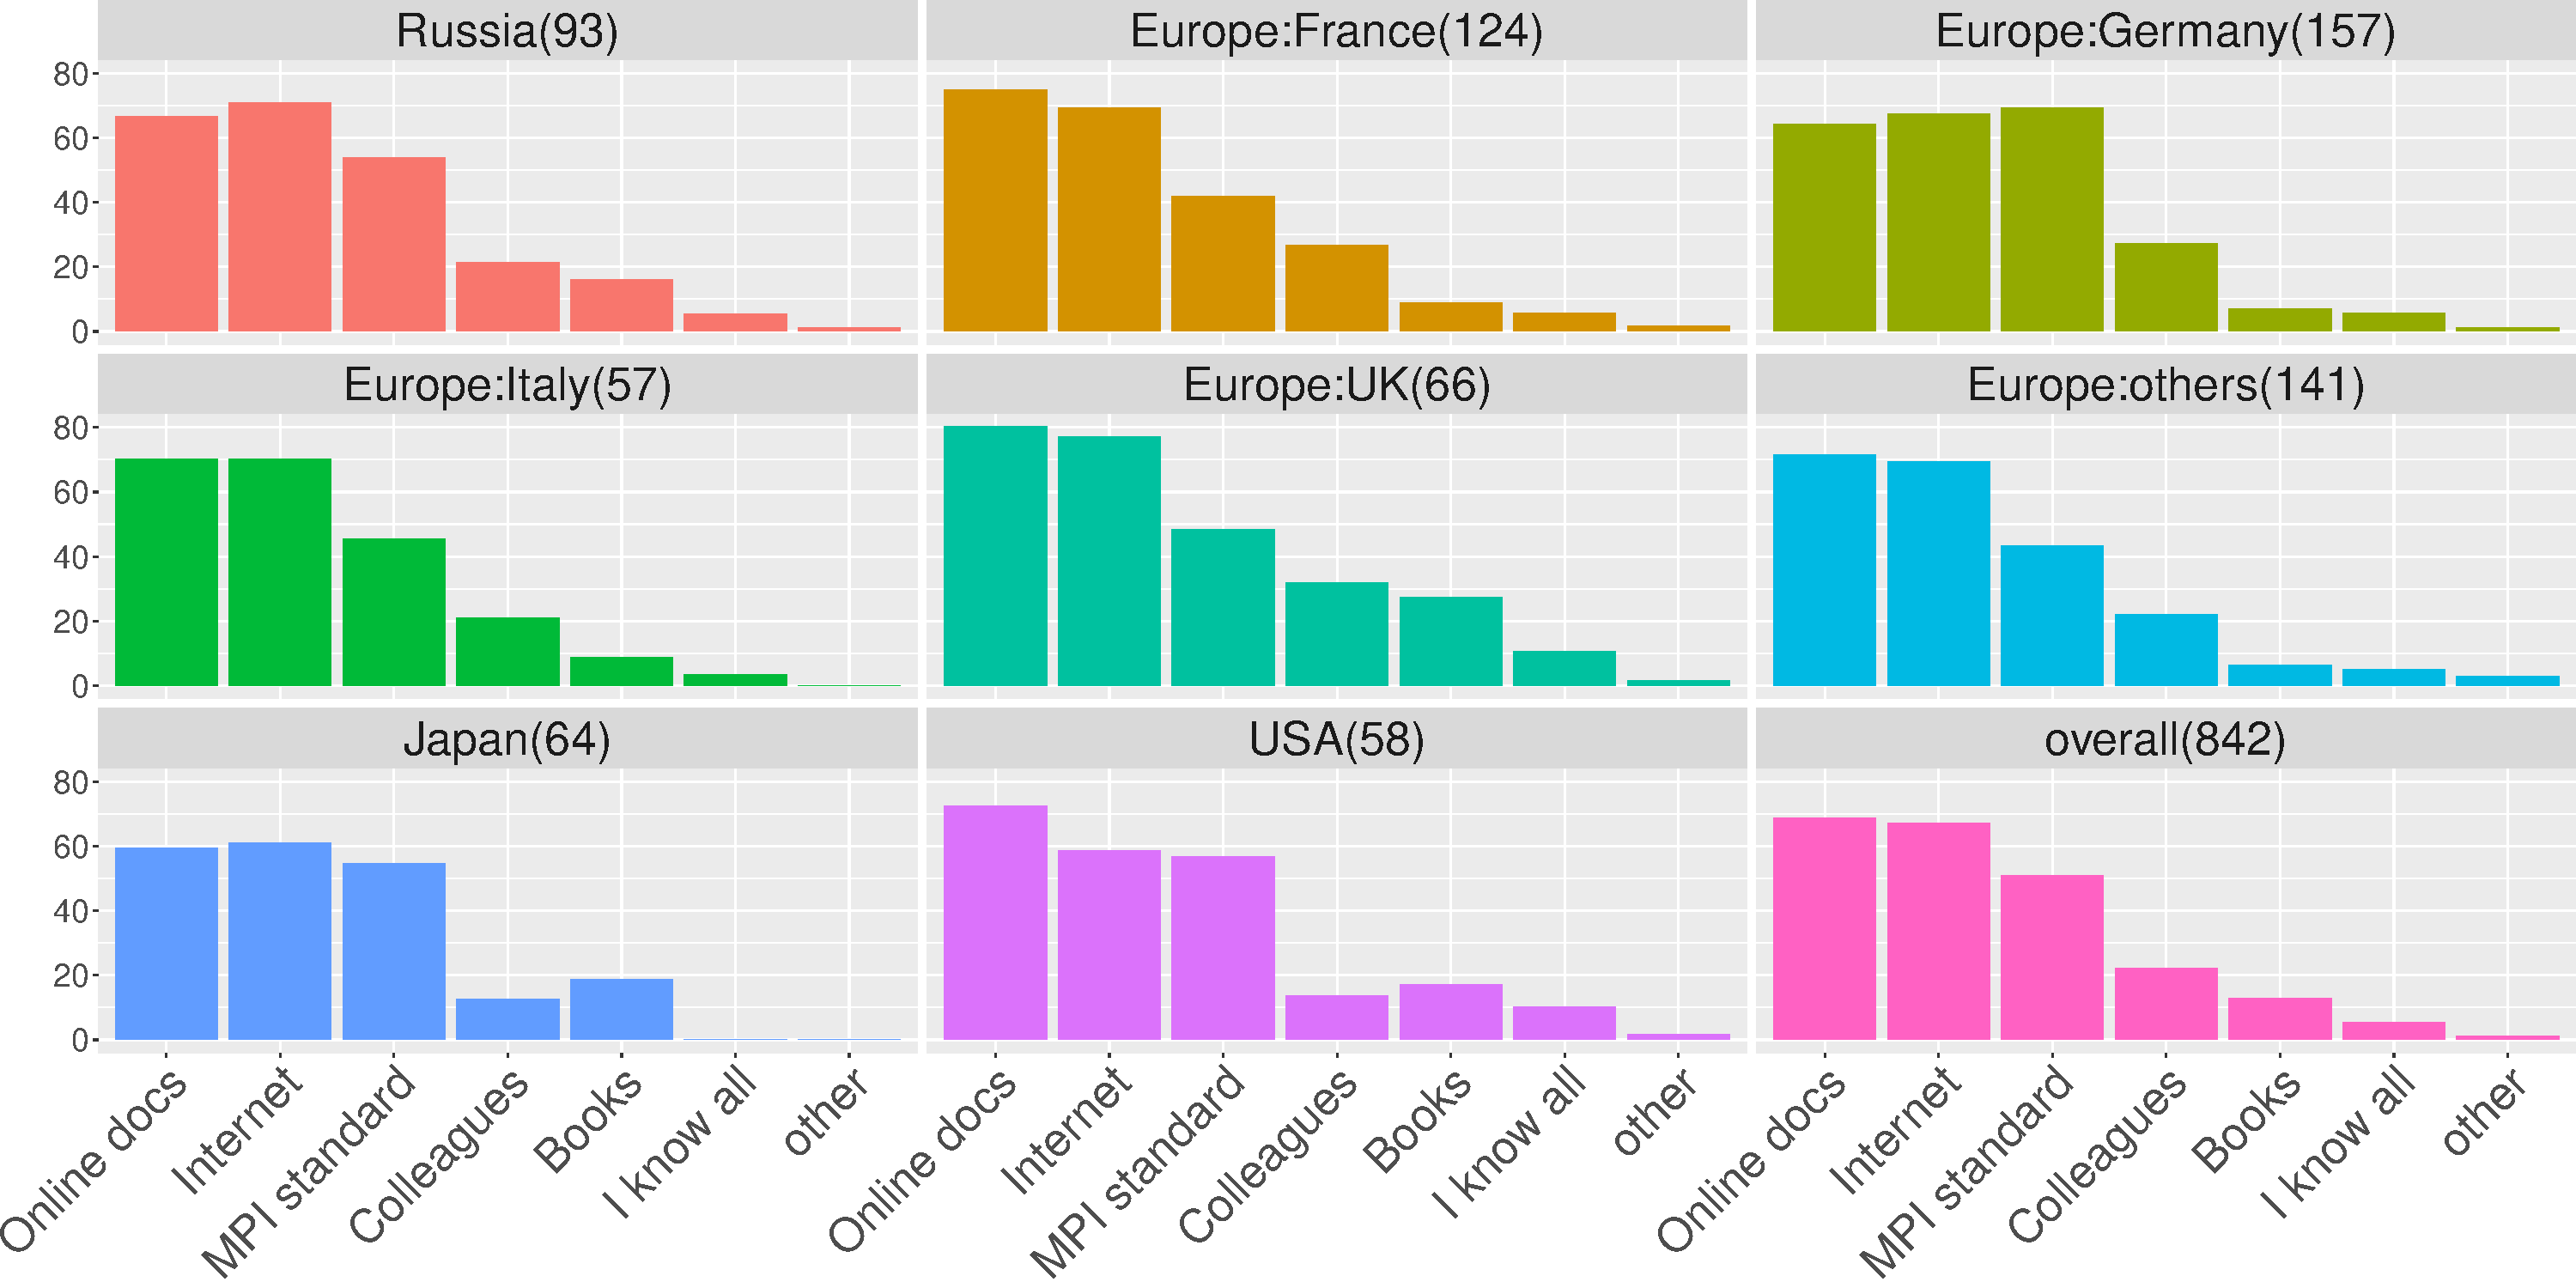
\includegraphics[width=8cm]{R-scripts/Q14.pdf}
\caption{Q14: Checking Specification {\it(multiple)}}
\label{fig:checking-spec}
\end{center}
\end{figure}

Currently the MPI standard documents are available in PDF format and
hardcover books~\cite{mpi-hardcover}. There are some MPI tutorial web
sites (\cite{mpi-tutorial} as an example). \cite{mpi-tutorial-intro}
pointed out most of such online documents are out-dated and not
thorough. It might be a good idea for MPI Forum to officially publish
some supplemental document(s) in another online hypertext form.

\begin{figure}[htb]
\begin{center}
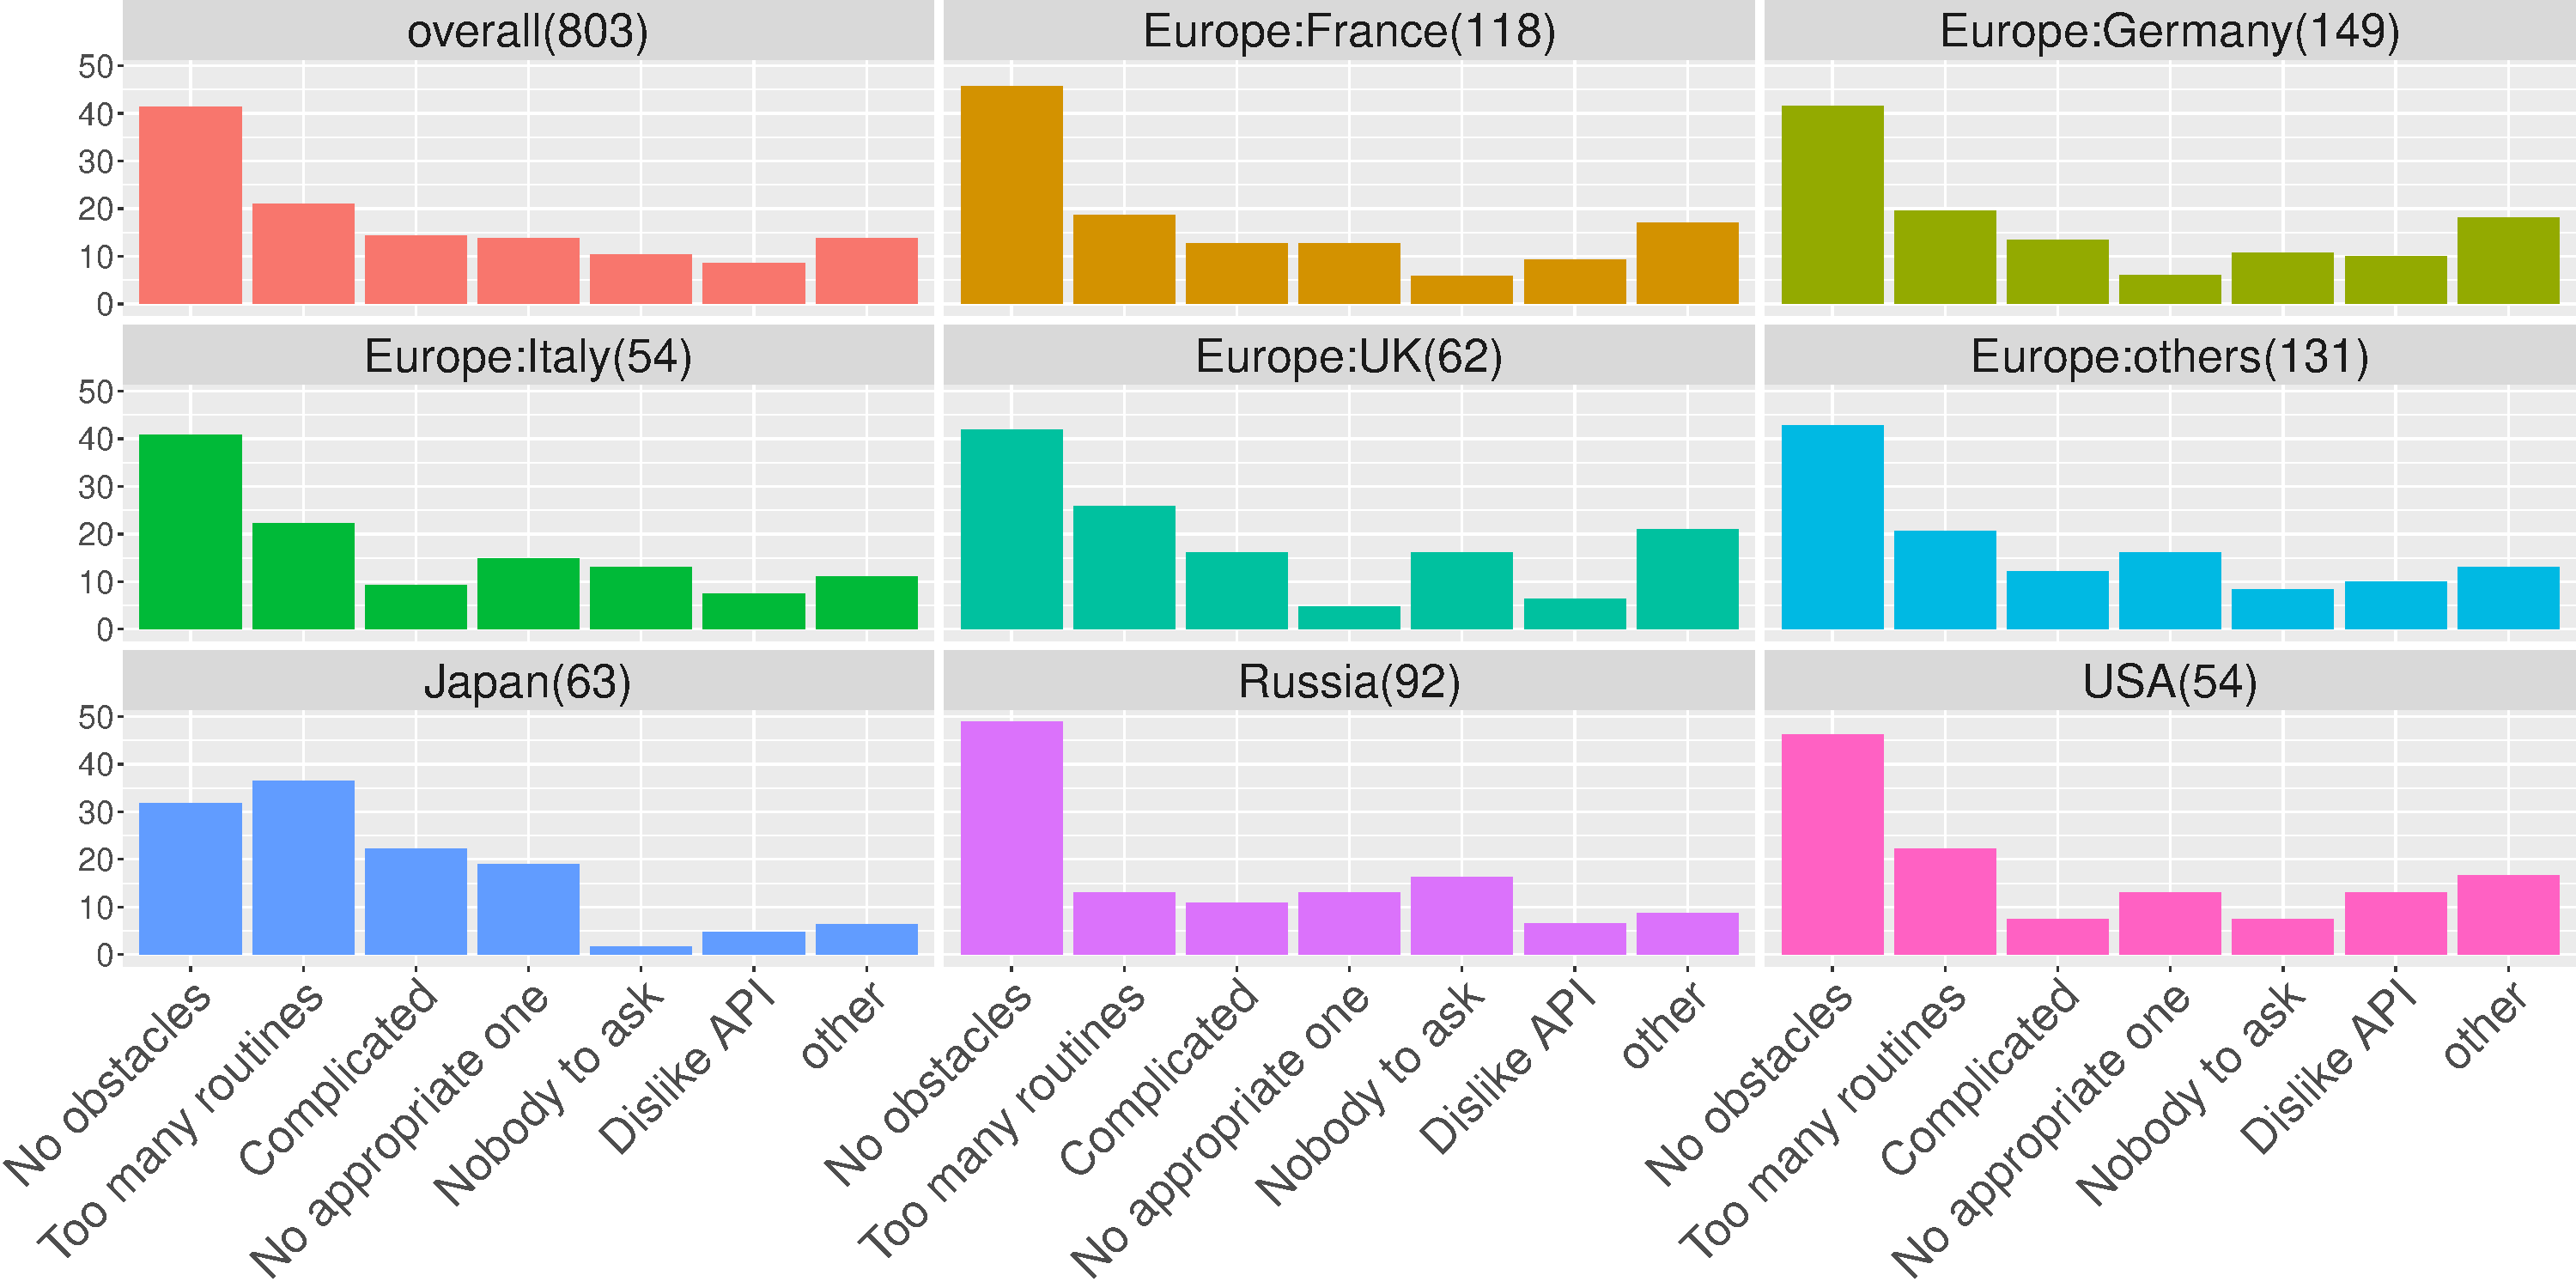
\includegraphics[width=8cm]{R-scripts/Q19.pdf}
\caption{Q19: Learning Obstacles {\it(multiple)}}
\label{fig:learning-obstacles}
\end{center}
\end{figure}

Generally speaking, there can be a case where a particular question in
a survey may ignite for participants to explode their dissatisfaction
by writing messages into a free text field. In our survey Q19 is
such a question. The 
largest number of \myquote{other} inputs in our survey can be found 
at Q19 asking ``What are your obstacles to mastering MPI?''
(Fig.~\ref{fig:learning-obstacles}). Although the largest answer is
the choice of \myquote{No obstacles,} we got 111 \myquote{other} inputs
exceptionally. Q4 and Q7 are the second largest (70), but these are
because of the variety of answers. 
More than 20 participants answered \myquote{other} raise
\myquote{time} (to master MPI). Many other participants pointed 
out the need of MPI programming guideline (\myquote{clear doc.},
\myquote{internal doc.}, \myquote{implementation 
  doc.}, \myquote{performance guideline}, and so on, in their words).
Some participants complaints about implementations and the
(performance or specification) differences among implementations.  

\begin{figure}[htb]
\begin{center}
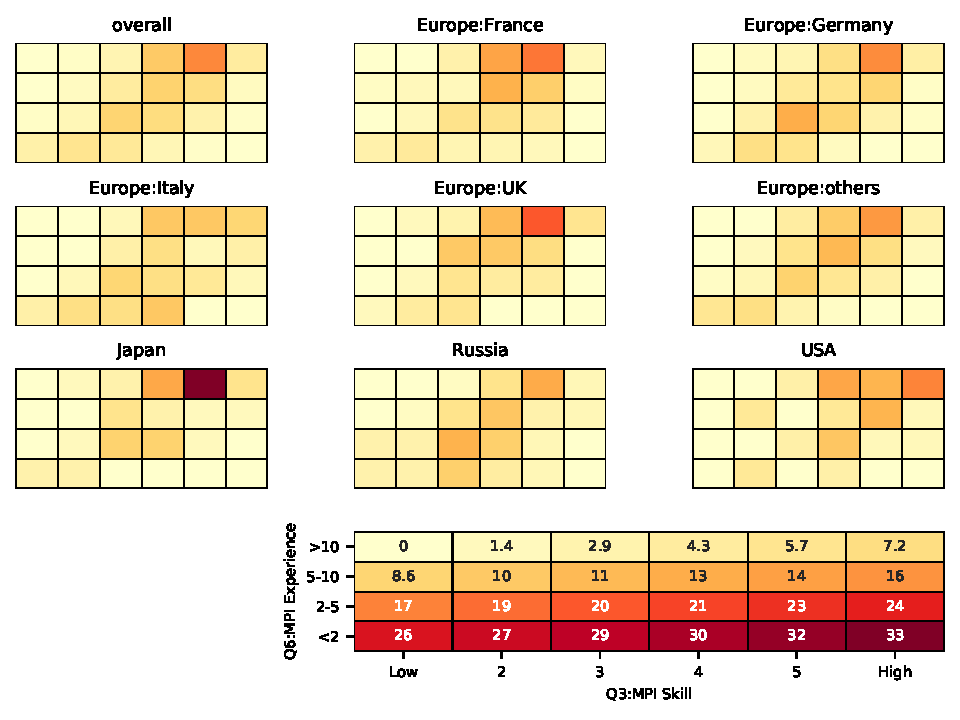
\includegraphics[width=8cm]{Figs/Q6-Q3.pdf}
\caption{Q6-Q3: MPI Experience {\it(single)} and MPI Skill {\it single}}
\label{fig:experience-and-skill}
\end{center}
\end{figure}

As shown in Fig.~\ref{fig:experience-and-skill}, the cross-tab heatmap
graphs between Q6 (Fig.~\ref{fig:mpi-experience} and Q3
(Fig.~\ref{fig:mpi-skill}, there is a strong correlation, from
lower-left to higher-right, between those
two questions regardless to countries or regions. And these graphs
tell that it takes more than 10 years of MPI programming experience to
get high MPI skill (\myquote{4} or \myquote{High}) in most counries
and regions. Many MPI users in US can get high (\myquote{4})
MPI skill in 5 to 10 years. Although this is shorter than the other
countries and regions, the tendency is the same.

\subsection{MPI Programming Difficulty and Tuning}

Fig.~\ref{fig:difficulty} shows the result of Q15 asking ``What is the
most difficult part of writing an MPI program?'' and
Fig~\ref{fig:tuning} shows the result of Q23 asking ``Is there any
room for performance tuning in your MPI programs?'' The largest part
of US and UK participants chose \myquote{algorithm design} whilst the
participants of the other countries and regions chose
\myquote{debugging}. In US, the second largest choice was
\myquote{Domain Decomposition}. In Japan, the second largest is
\myquote{Tuning}. 

\begin{figure}[htb]
\begin{center}
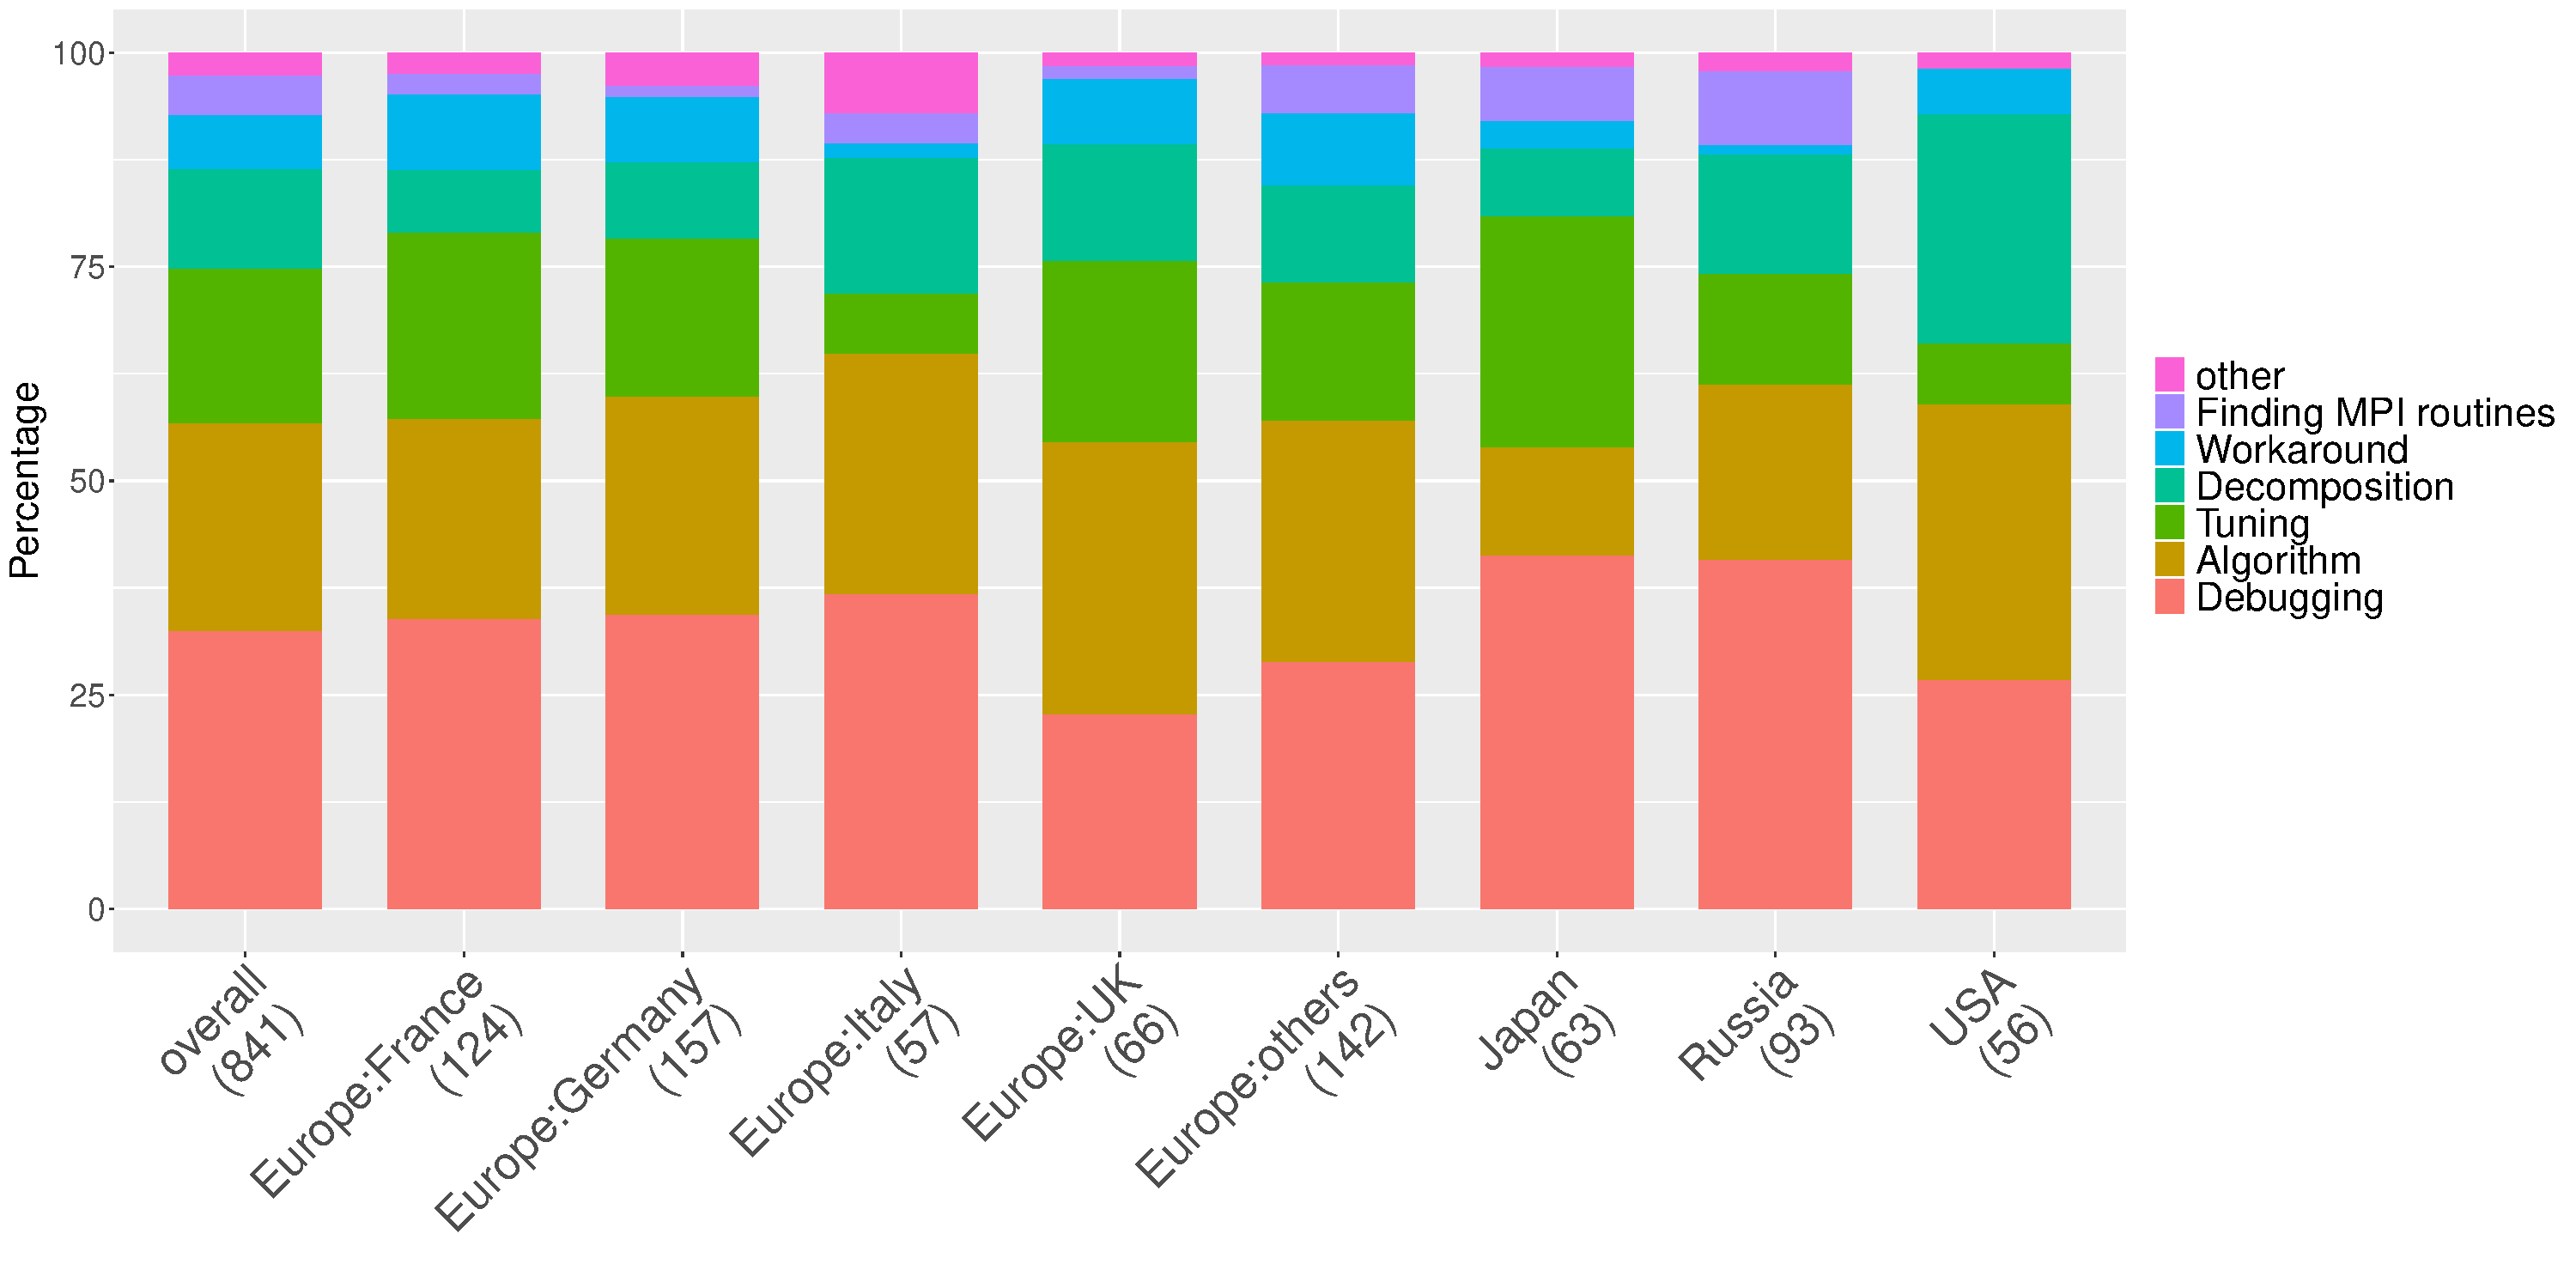
\includegraphics[width=9cm]{R-scripts/Q15.pdf}
\caption{Q15: MPI Programming Difficulty {\it(single)}}
\label{fig:difficulty}
\end{center}
\end{figure}

Fig.~\ref{fig:tuning} has more divergence than
Fig~\ref{fig:difficulty}. The participants selected \myquote{my MPI
  programs are well-tuned} is only around 10\% excepting Japan and
Russia. There seems to be a lots of room to tune MPI programs in
general, however, around 40\% of participants said they do not have
enough resource to do that. In Japan, the percentage of well-tuned
program is only few percent. Contrastingly, Russian percentage of
choosing \myquote{well-tuned} is the highest among the countries and
regions. 

\begin{figure}[htb]
\begin{center}
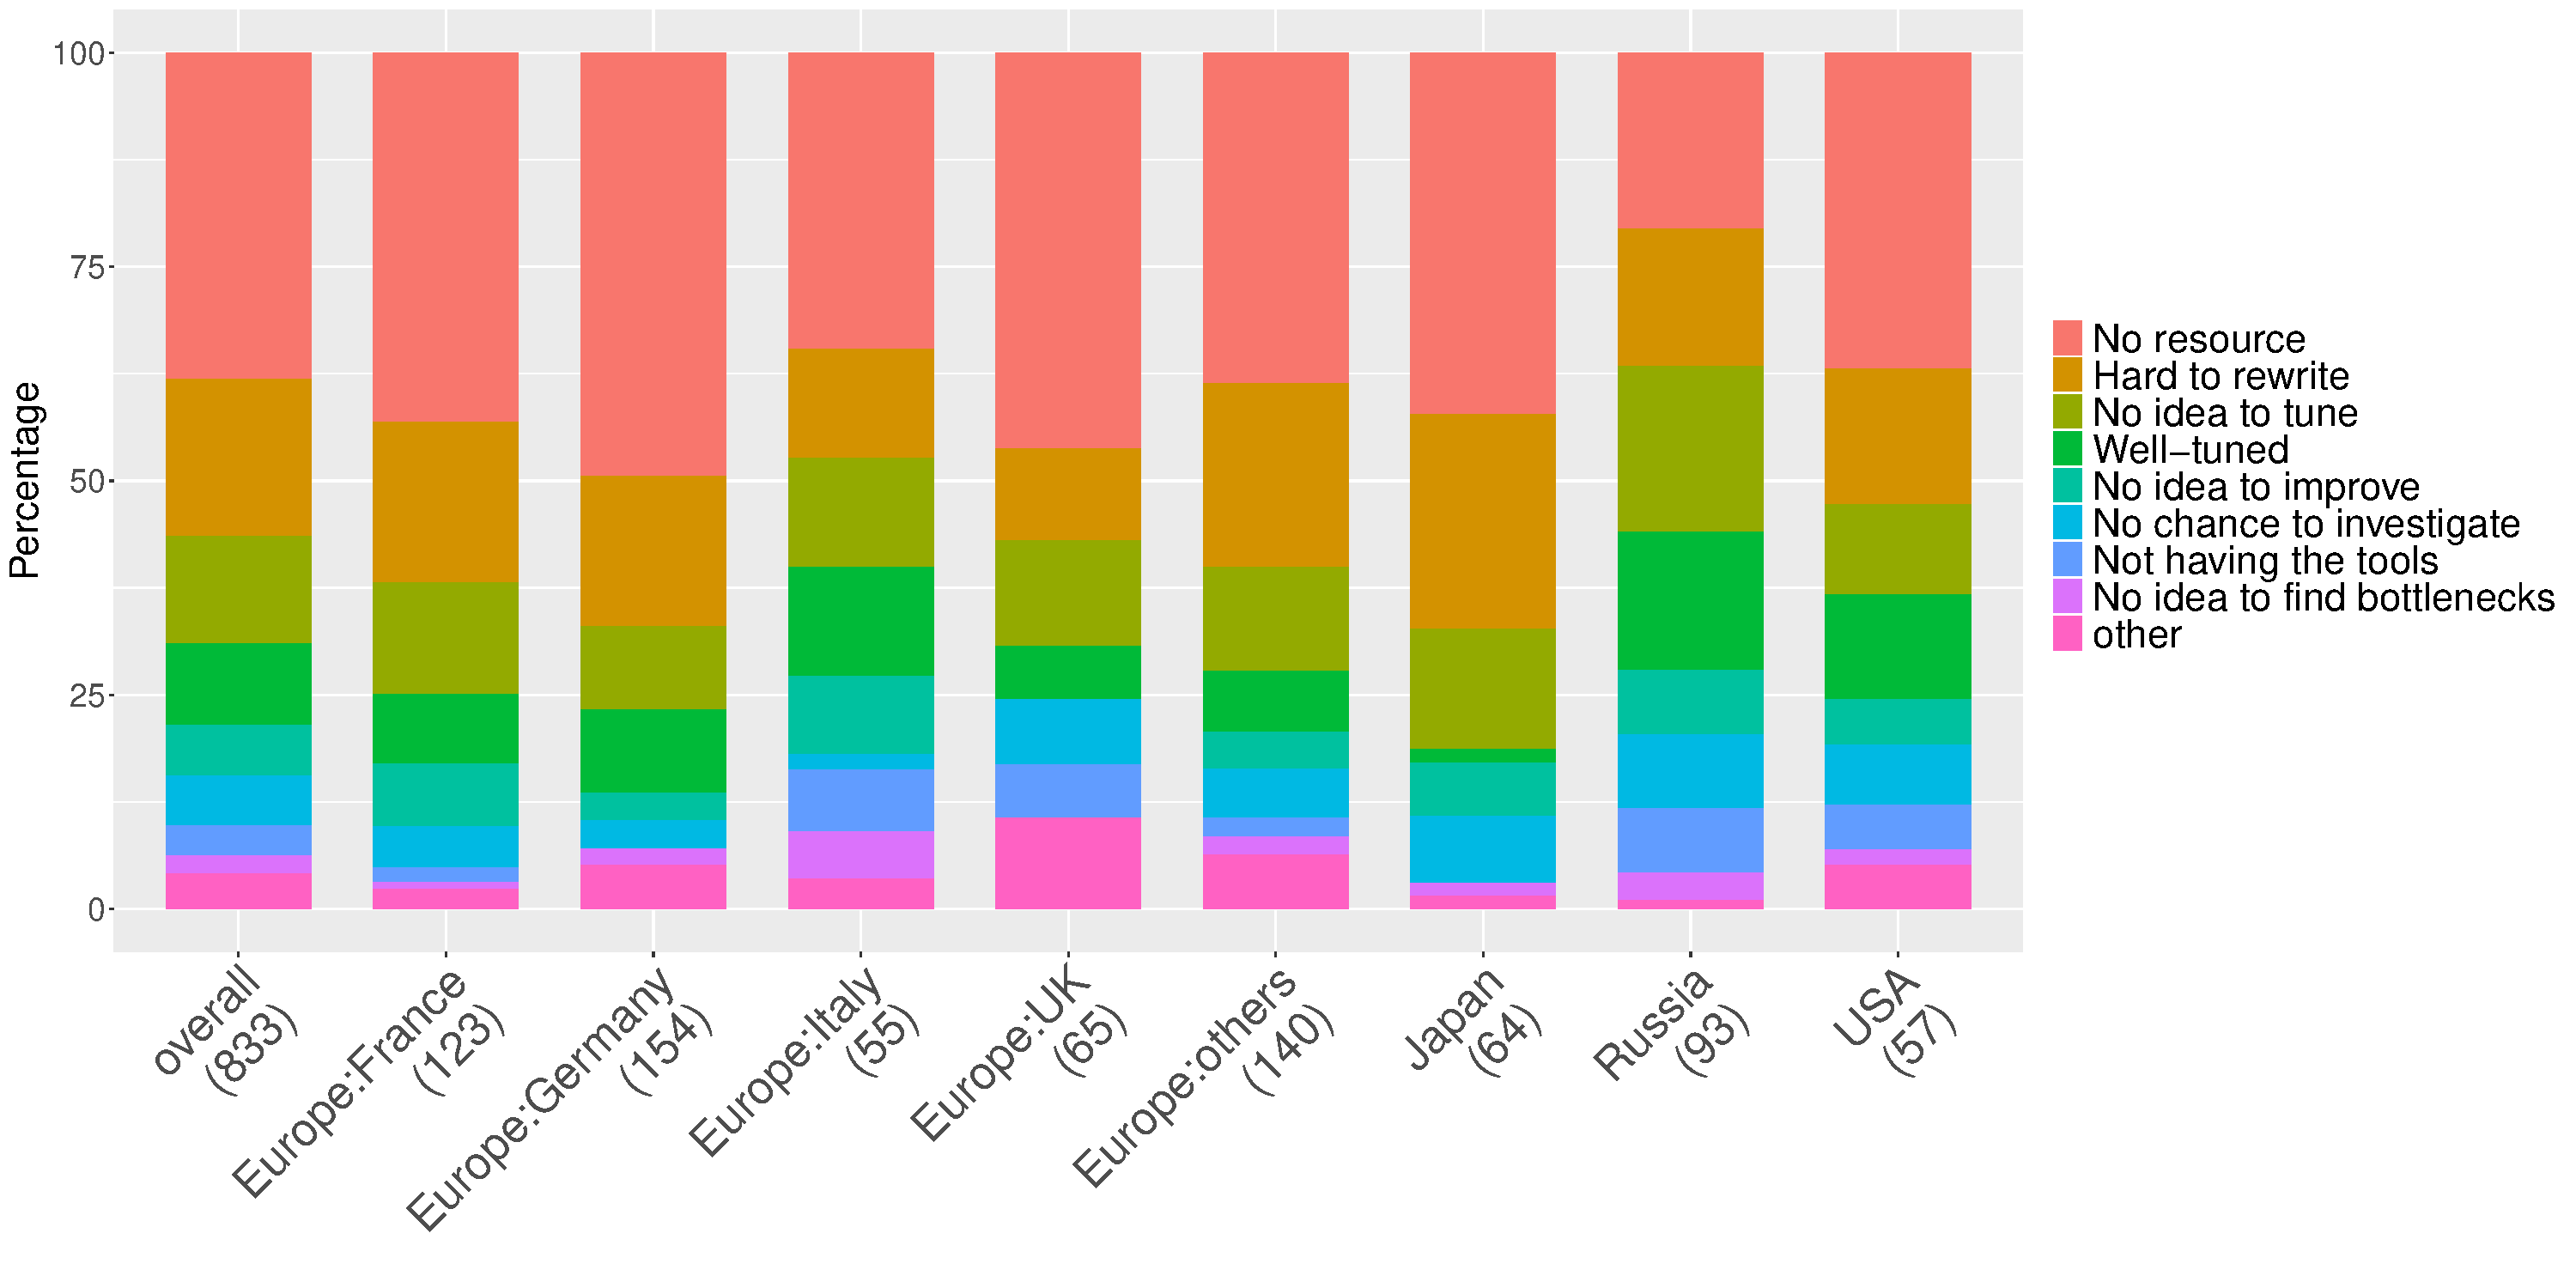
\includegraphics[width=9cm]{R-scripts/Q23.pdf}
\caption{Q23: Performance Tuning {\it(single)}}
\label{fig:tuning}
\end{center}
\end{figure}

\subsection{MPI+X and Alternatives}

Fig.~\ref{fig:mpi-x} shows the result of Q22 asking ``Have you ever
written MPI+''X'' programs?'' Most participants have the experiences of
writing MPI+OpenMP programs. \myquote{CUDA} is the second largest in
US and the percentage of \myquote{No} in US is the lowest among the
others. Considering the low percentage of \myquote{No} (approx.
25\% in overall), most participants using MPI with something else.
\cite{10.1145/3295500.3356176} reported that the approximately 3/4 of
the target programs use the hybrid model of MPI+OpenMP. This percentage
is very close to our survey result.

\begin{figure}[htb]
\begin{center}
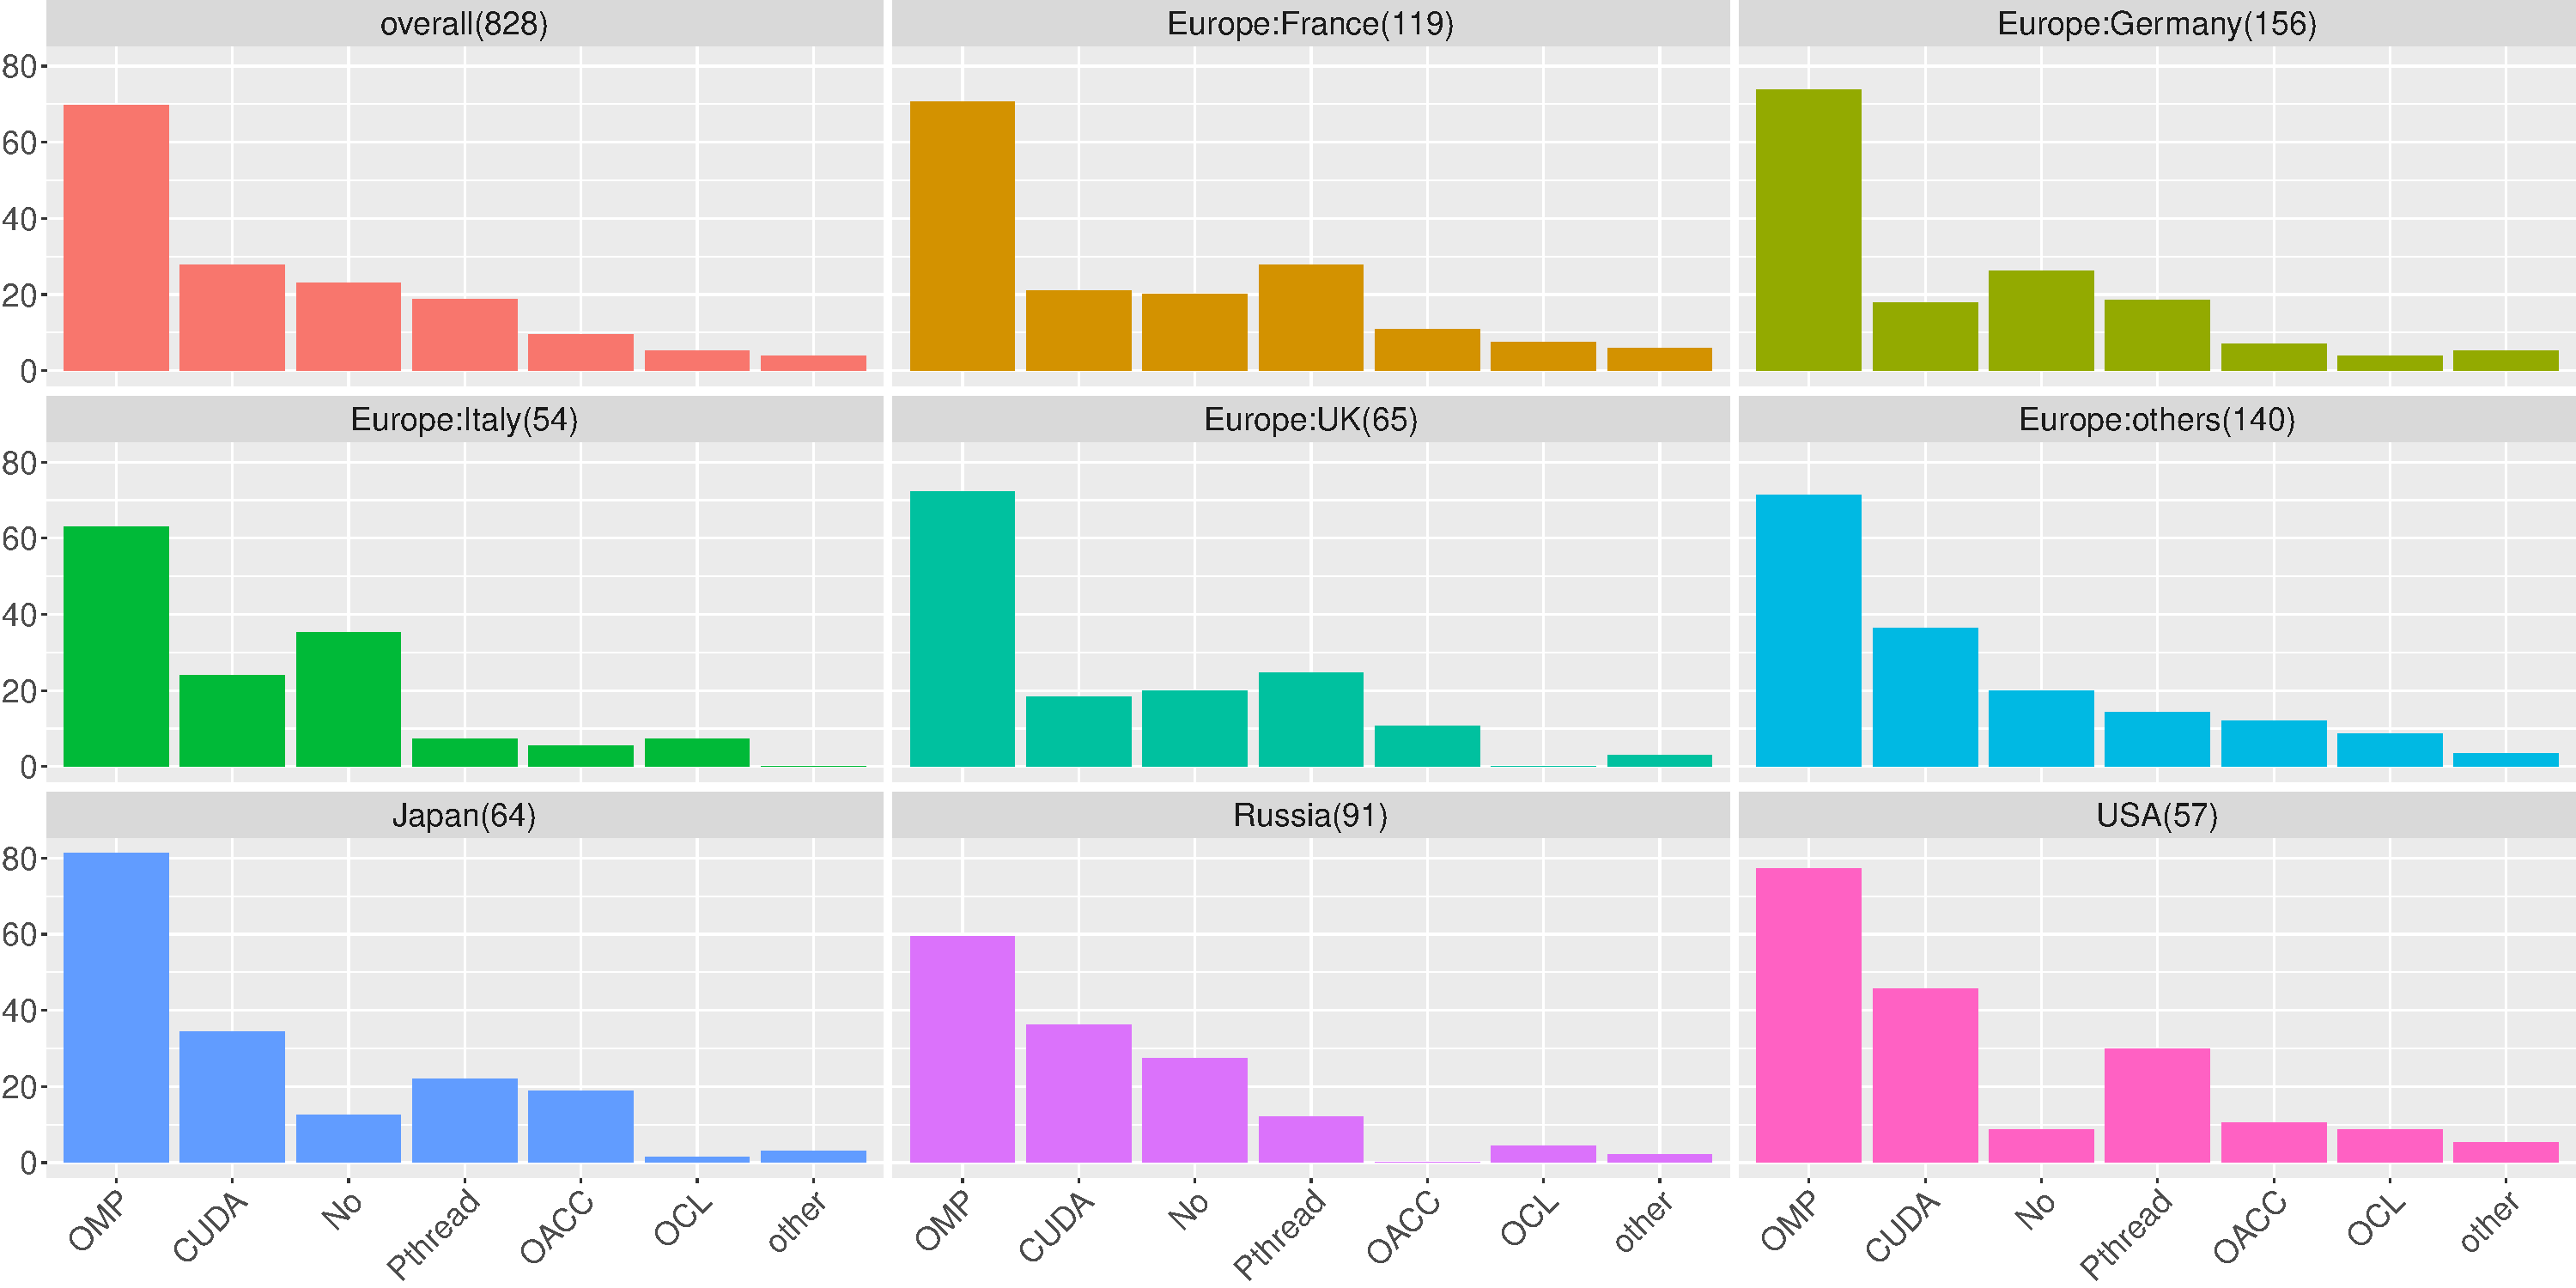
\includegraphics[width=8cm]{R-scripts/Q22.pdf}
\caption{Q22: MPI+X {\it(multiple)}}
\label{fig:mpi-x}
\end{center}
\end{figure}

\begin{figure}[htb]
\begin{center}
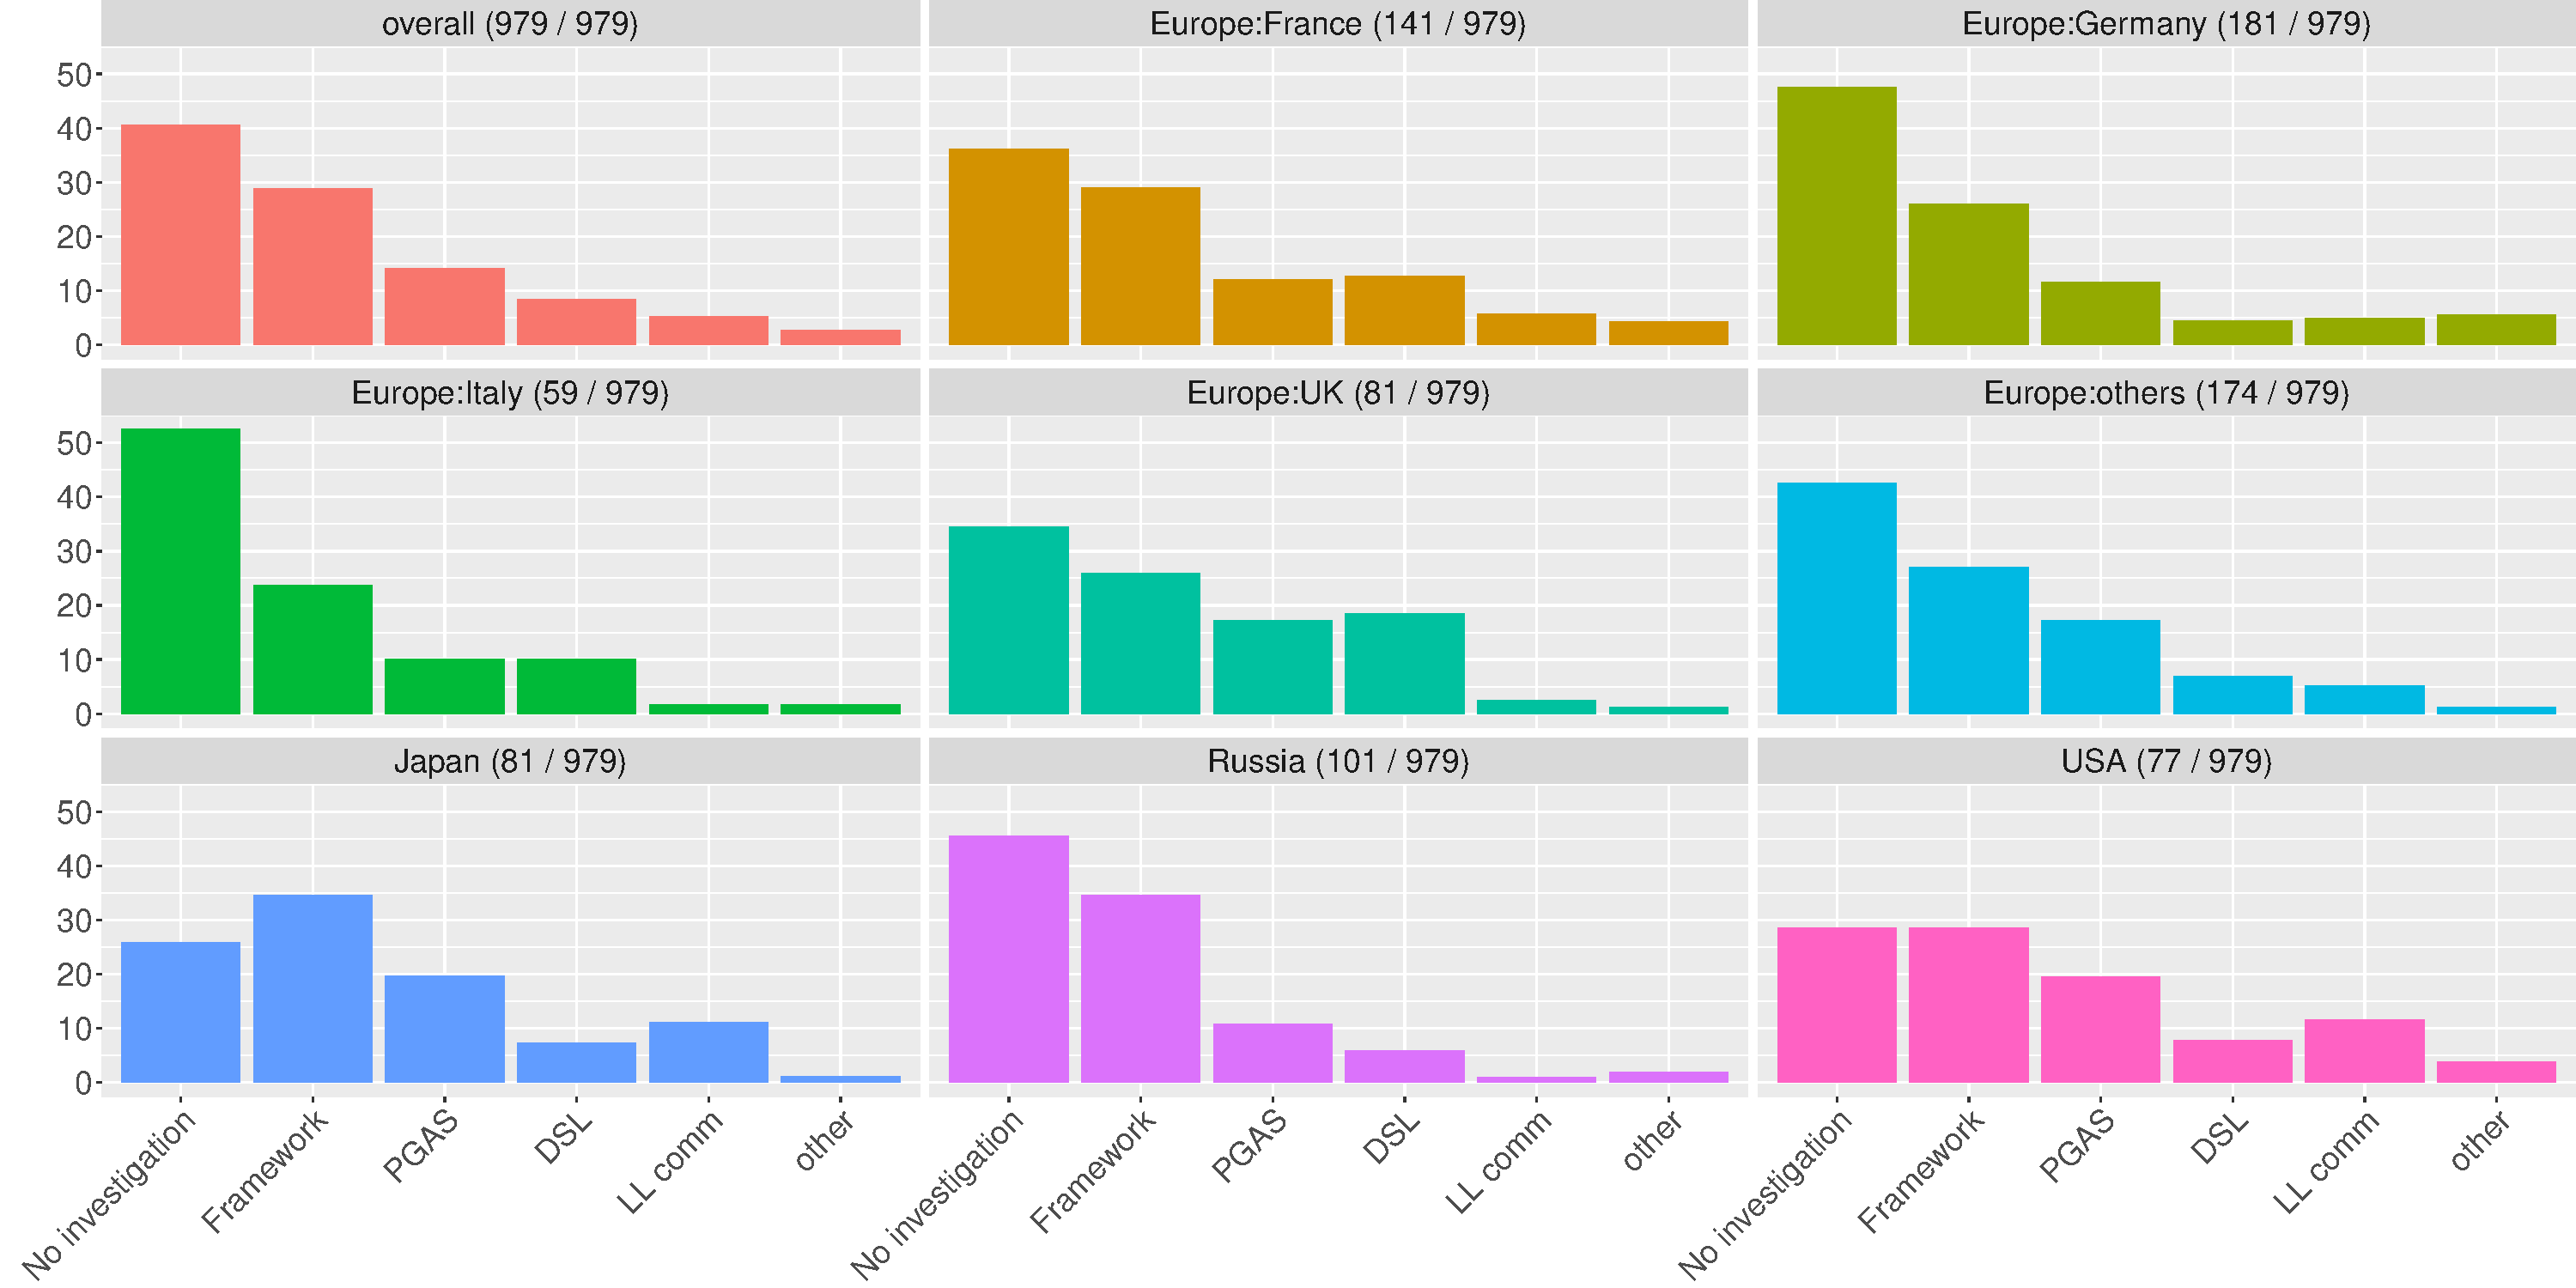
\includegraphics[width=8cm]{R-scripts/Q24.pdf}
\caption{Q24: MPI Alternatives {\it(multiple)}}
\label{fig:mpi-alternatives}
\end{center}
\end{figure}

When the participants were asked the question ``What, if any,
alternatives are you investigating to indirectly call MPI or another
communication layer by using another parallel language/library?'' they
exhibited as shown in Fig.~\ref{fig:mpi-alternatives}. In overall,
almost half participants do not investigate the alternatives. The second
largest answer was \myquote{Framework} (i.e. a framework or library
using MPI) followed by \myquote{PGAS}. The
differences over the countries and regions are not so big. 
  
\begin{figure}[htb]
\begin{center}
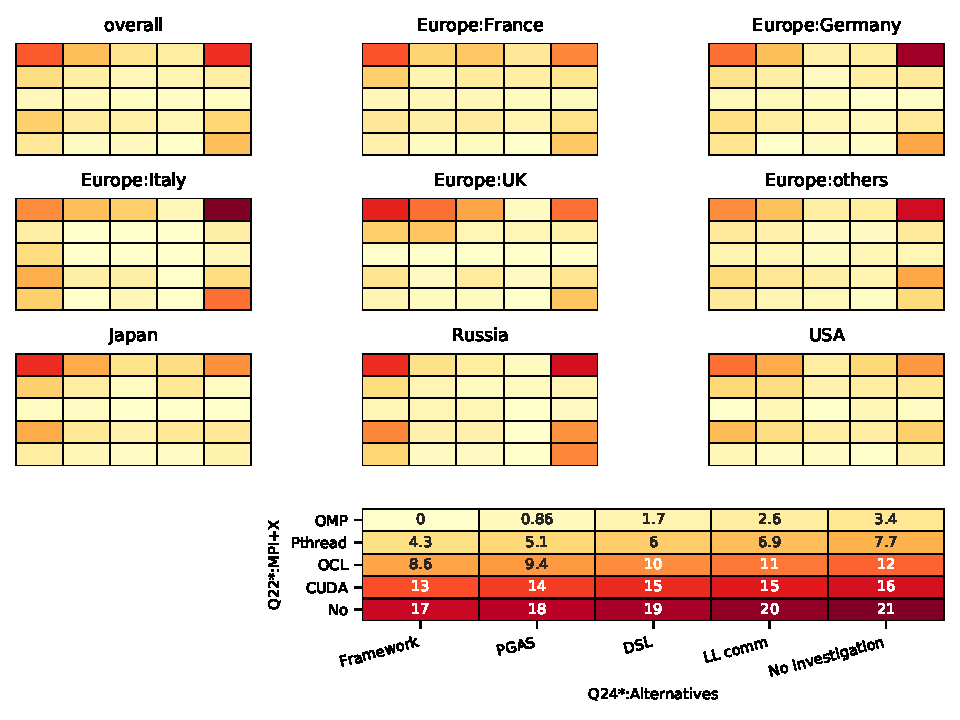
\includegraphics[width=8cm]{Figs/Q22-Q24.pdf}
\caption{Q22-Q24: MPI+X {\it(multiple)} and MPI Alternatives {\it(multiple)}}
\label{fig:mpi-x-and-alternatives}
\end{center}
\end{figure}

Fig.~\ref{fig:mpi-x-and-alternatives} shows the cross-tab analysis of
the above Q22 and Q24. A certain percentage of participants of
Germany, Italy, Russia and other European countries using MPI+OpenMP
without investigating the MPI alternative (upper right corners of the
heatmaps in the figure). 

\subsection{Missing Features and Semantics}

It is a general concern how MPI provides optimization
opportunities in terms of hardware capabilities such as being able to
handle the various topologies of hardware components more 
efficiently. To answer this, Q25 asking ``If there were one
communication aspect which is not enough in the current MPI could
improve the performance of your application, what would you
prioritize? Or $\cdots$'' (Fig.~\ref{fig:mmissing-features}, full
question can be found at Appendix~\ref{app:questions}), and Q26 asking
``Is MPI providing all the communication semantics required by your
application? If not, what is missing?''
(Fig.~\ref{fig:missing-semantics}) were prepared. 

In Fig.~\ref{fig:missing-features}, only 23\% of overall MPI users
are satisfied with the current situation.
Interestingly enough the second largest percentage is
\myquote{additional comm. opt.} (\myquote{Additional optimization
  opportunities in terms of communication (network topology awareness,
  etc.)}, followed by \myquote{Multi-thread} and \myquote{Other
  opt.} (\myquote{Optimization opportunities except communication
  (architecture awareness, dynamic processing, accelerator support,
  etc.)}). 

\begin{figure}[htb]
\begin{center}
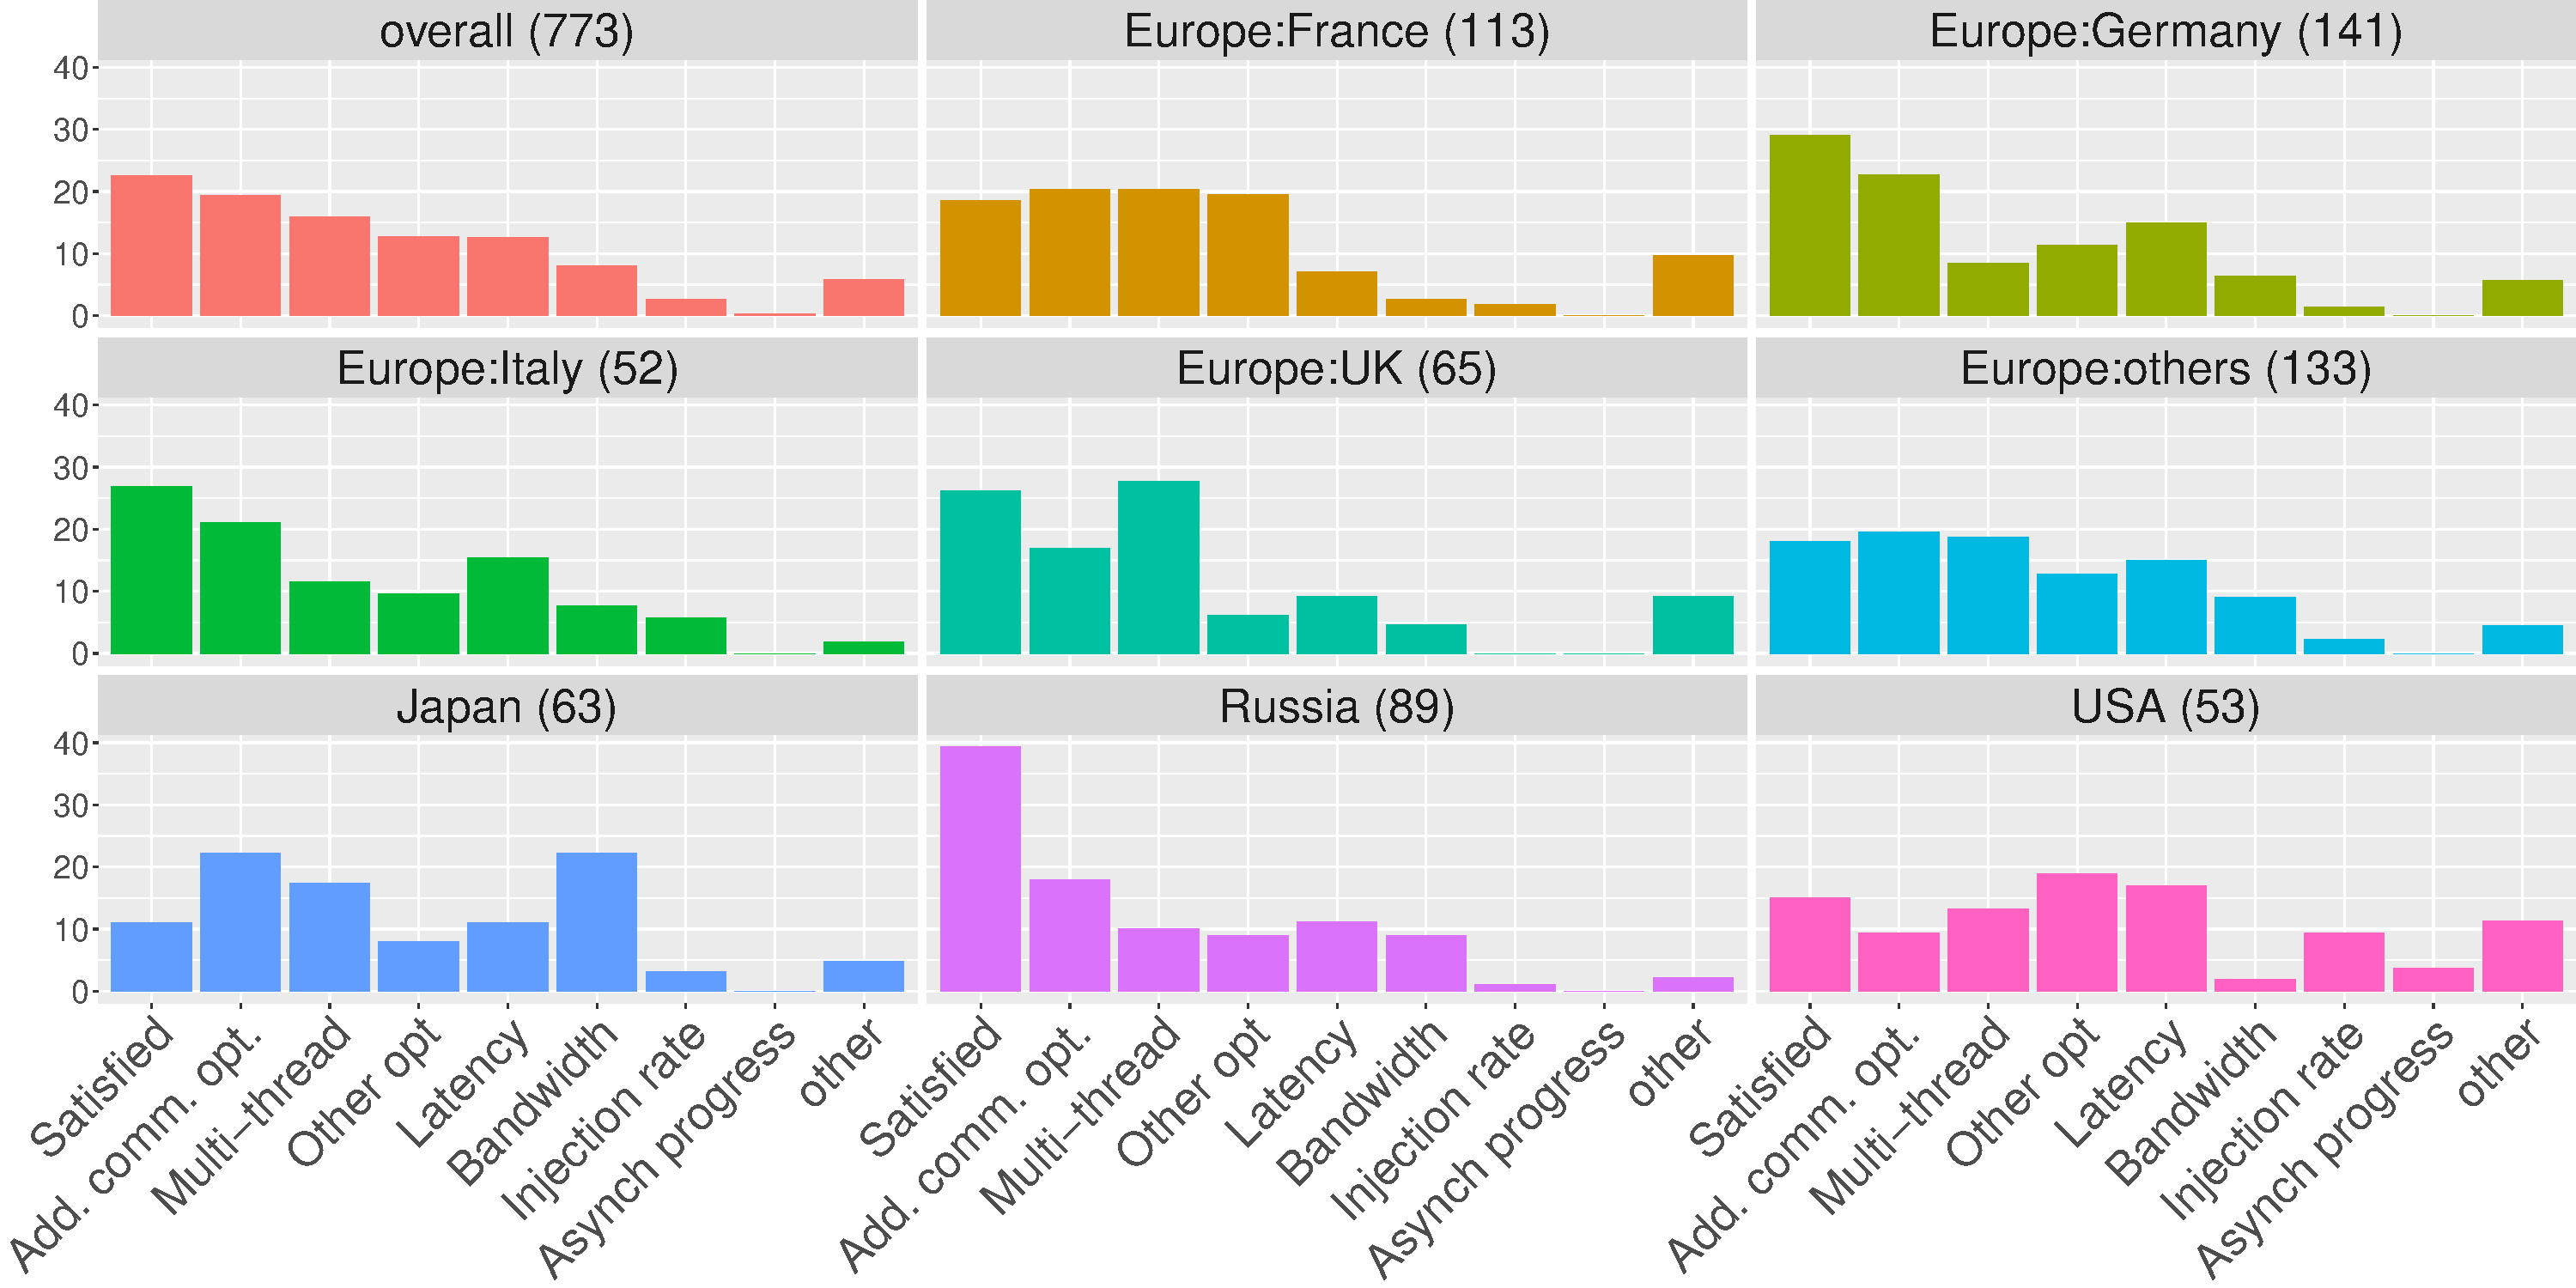
\includegraphics[width=8cm]{R-scripts/Q25.pdf}
\caption{Q25: Missing Features {\it(single)}}
\label{fig:missing-features}
\end{center}
\end{figure}

Q26 is somewhat similar to Q25, but asking more precise questions.
This question tackles the issue on which semantic 
feature is missing from MPI. Overall a very similar picture emerges
with Q25,
almost one third of the participants are satisfied with the current
situation. There is a high discrepancy between Japan where users are
the least satisfied with the current situation and Russia which are the most
satisfied. The same situation can be seen in Q25. The highest given
answer concerns \myquote{Add. opt} (\myquote{Additional optimization
  opportunities in terms of communication (topology awareness,
  locality, etc.)}). This is coherent with Q25 and managing
efficiently the topology seem a major concern to many users. Then
comes the concerns about the lack of 
resilience, a concern shared by more than 20\% of the
participants. Hiding latency through generalization of asynchrony over
the whole set of functions is another point raised repeatedly. 16\% of
the users think that a simpler and easier API would be 
 desirable (a topic where the discrepancy between different regions is
 minimal). 

\begin{figure}[htb]
\begin{center}
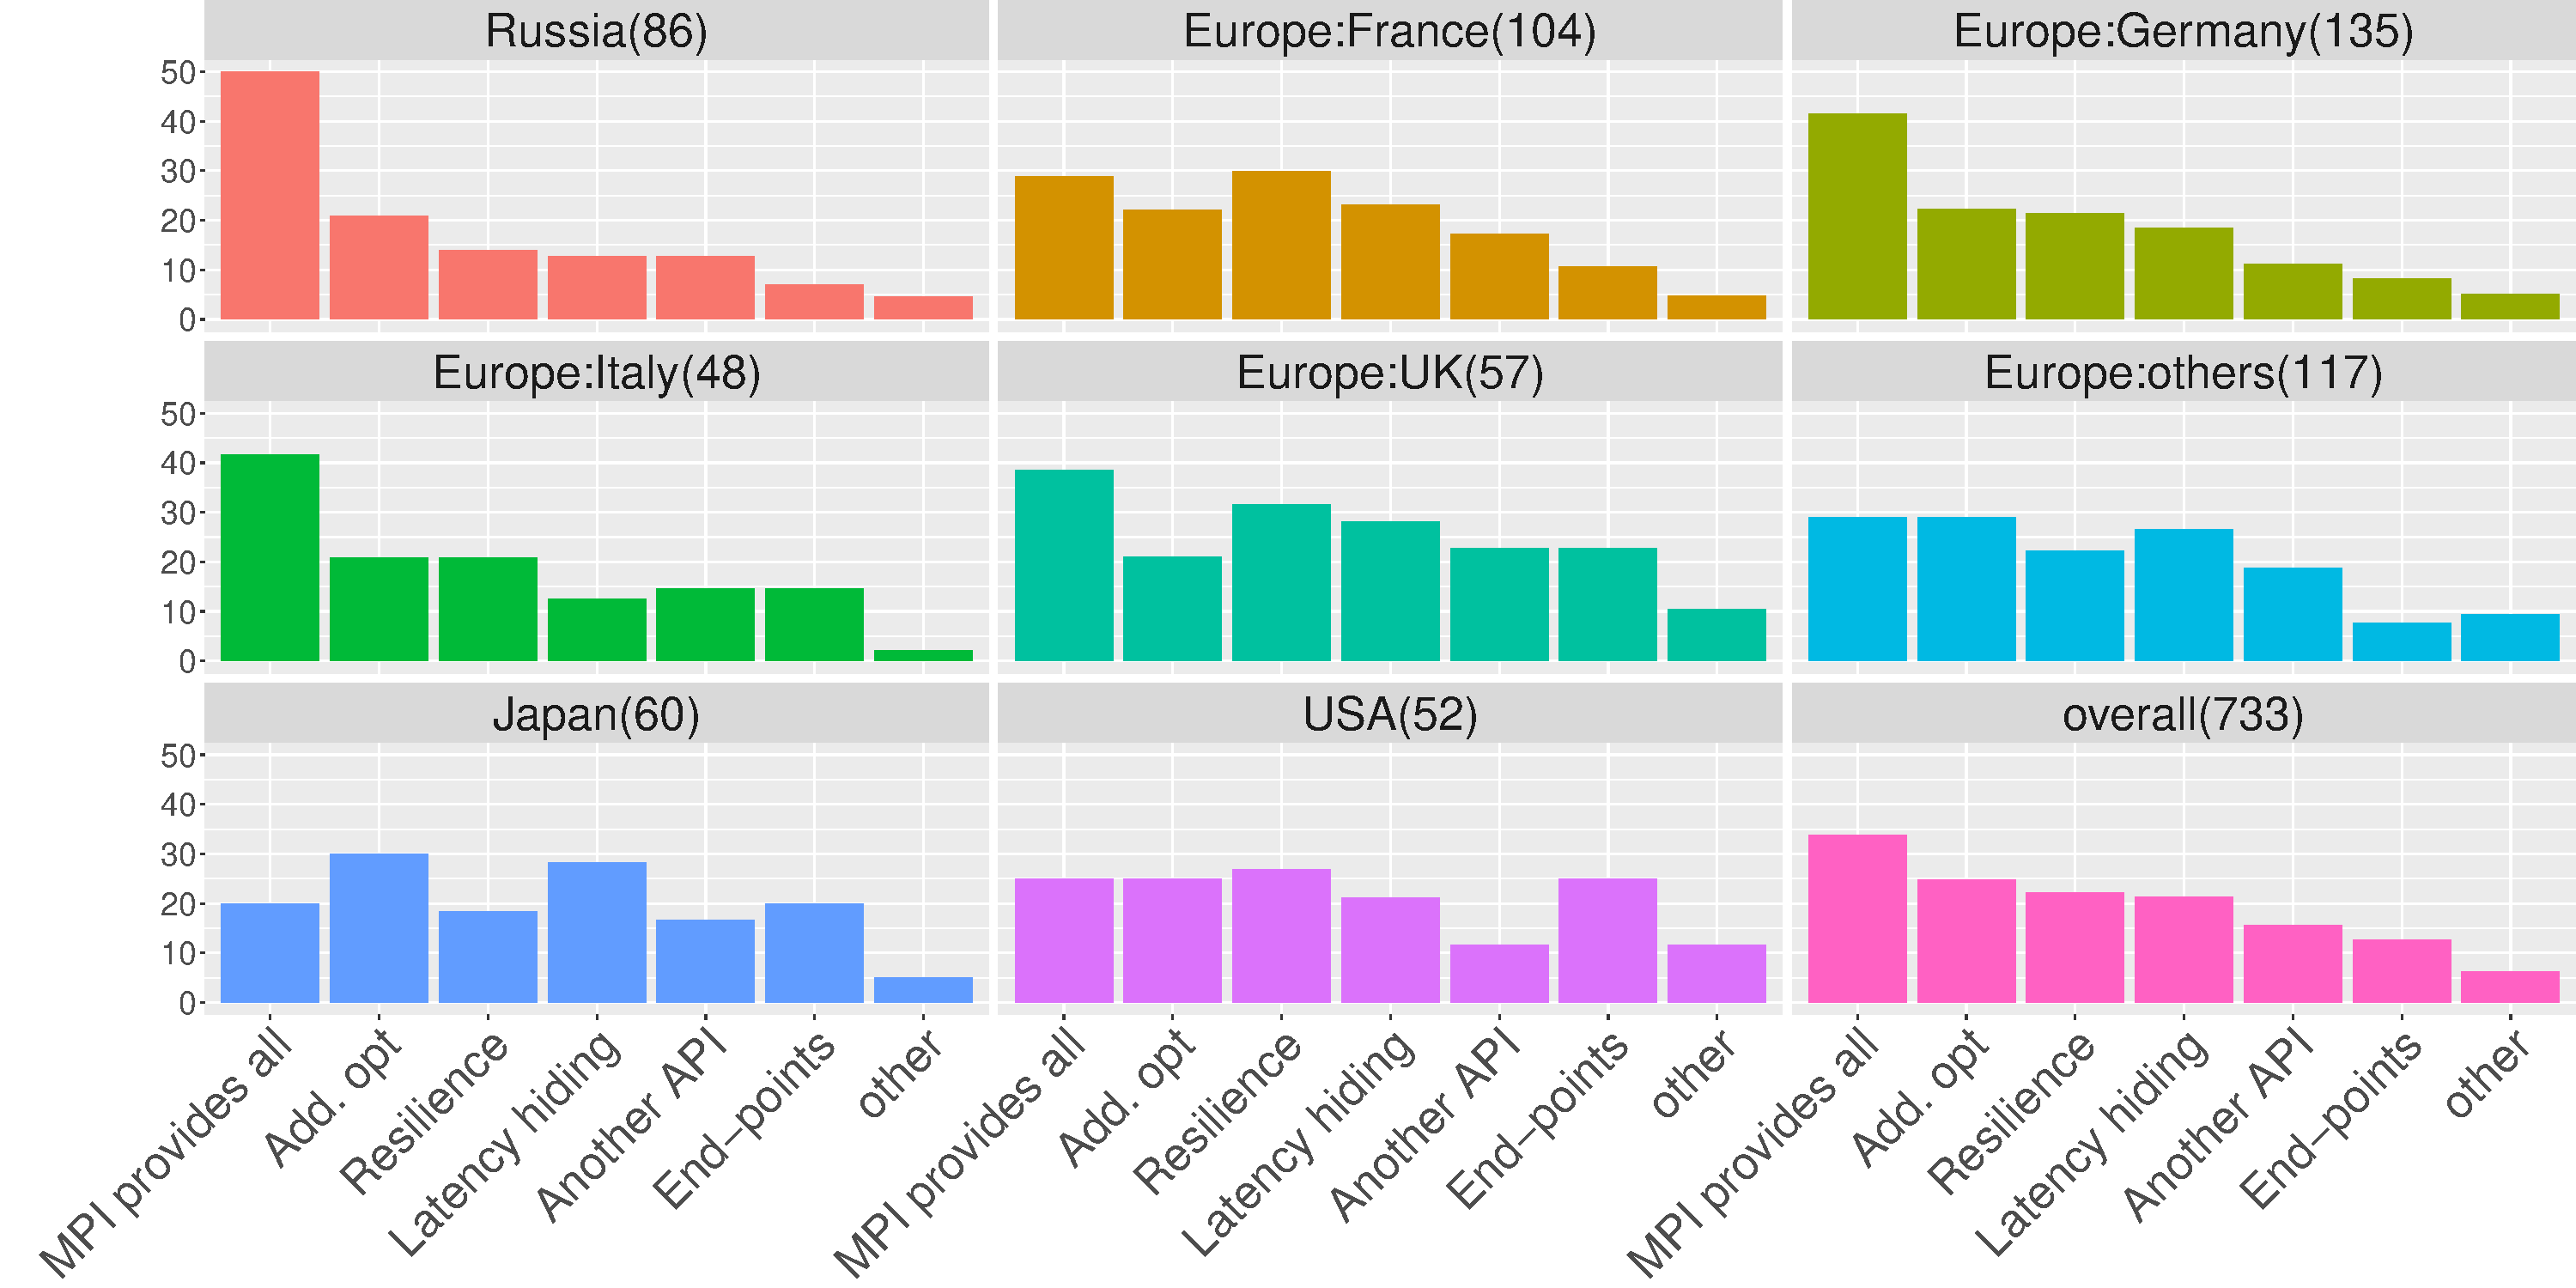
\includegraphics[width=8cm]{R-scripts/Q26.pdf}
\caption{Q26: MPI Semantics {\it(multiple)}}
\label{fig:missing-semantics}
\end{center}
\end{figure}

Finally, the least desired feature concerns the notion of endpoints,
as discussed in the MPI standardization effort. However taking in
account the extremely 
technical aspect of this question, and it's intricate evolution in the
standard, it might be possible that most people answering this
question knew little, and possible imprecisely, what this feature was
exactly about. 

It is very interesting that most countries concern about the
resilience (as Emmauel noted above). Although there are relatively big
disparity in the satisfaction (answering \myquote{MPI provides all}),
the disparities of the other answers are smaller. 

\comment{
\subsection{MPI communication}

\begin{figure}[htb]
\begin{center}
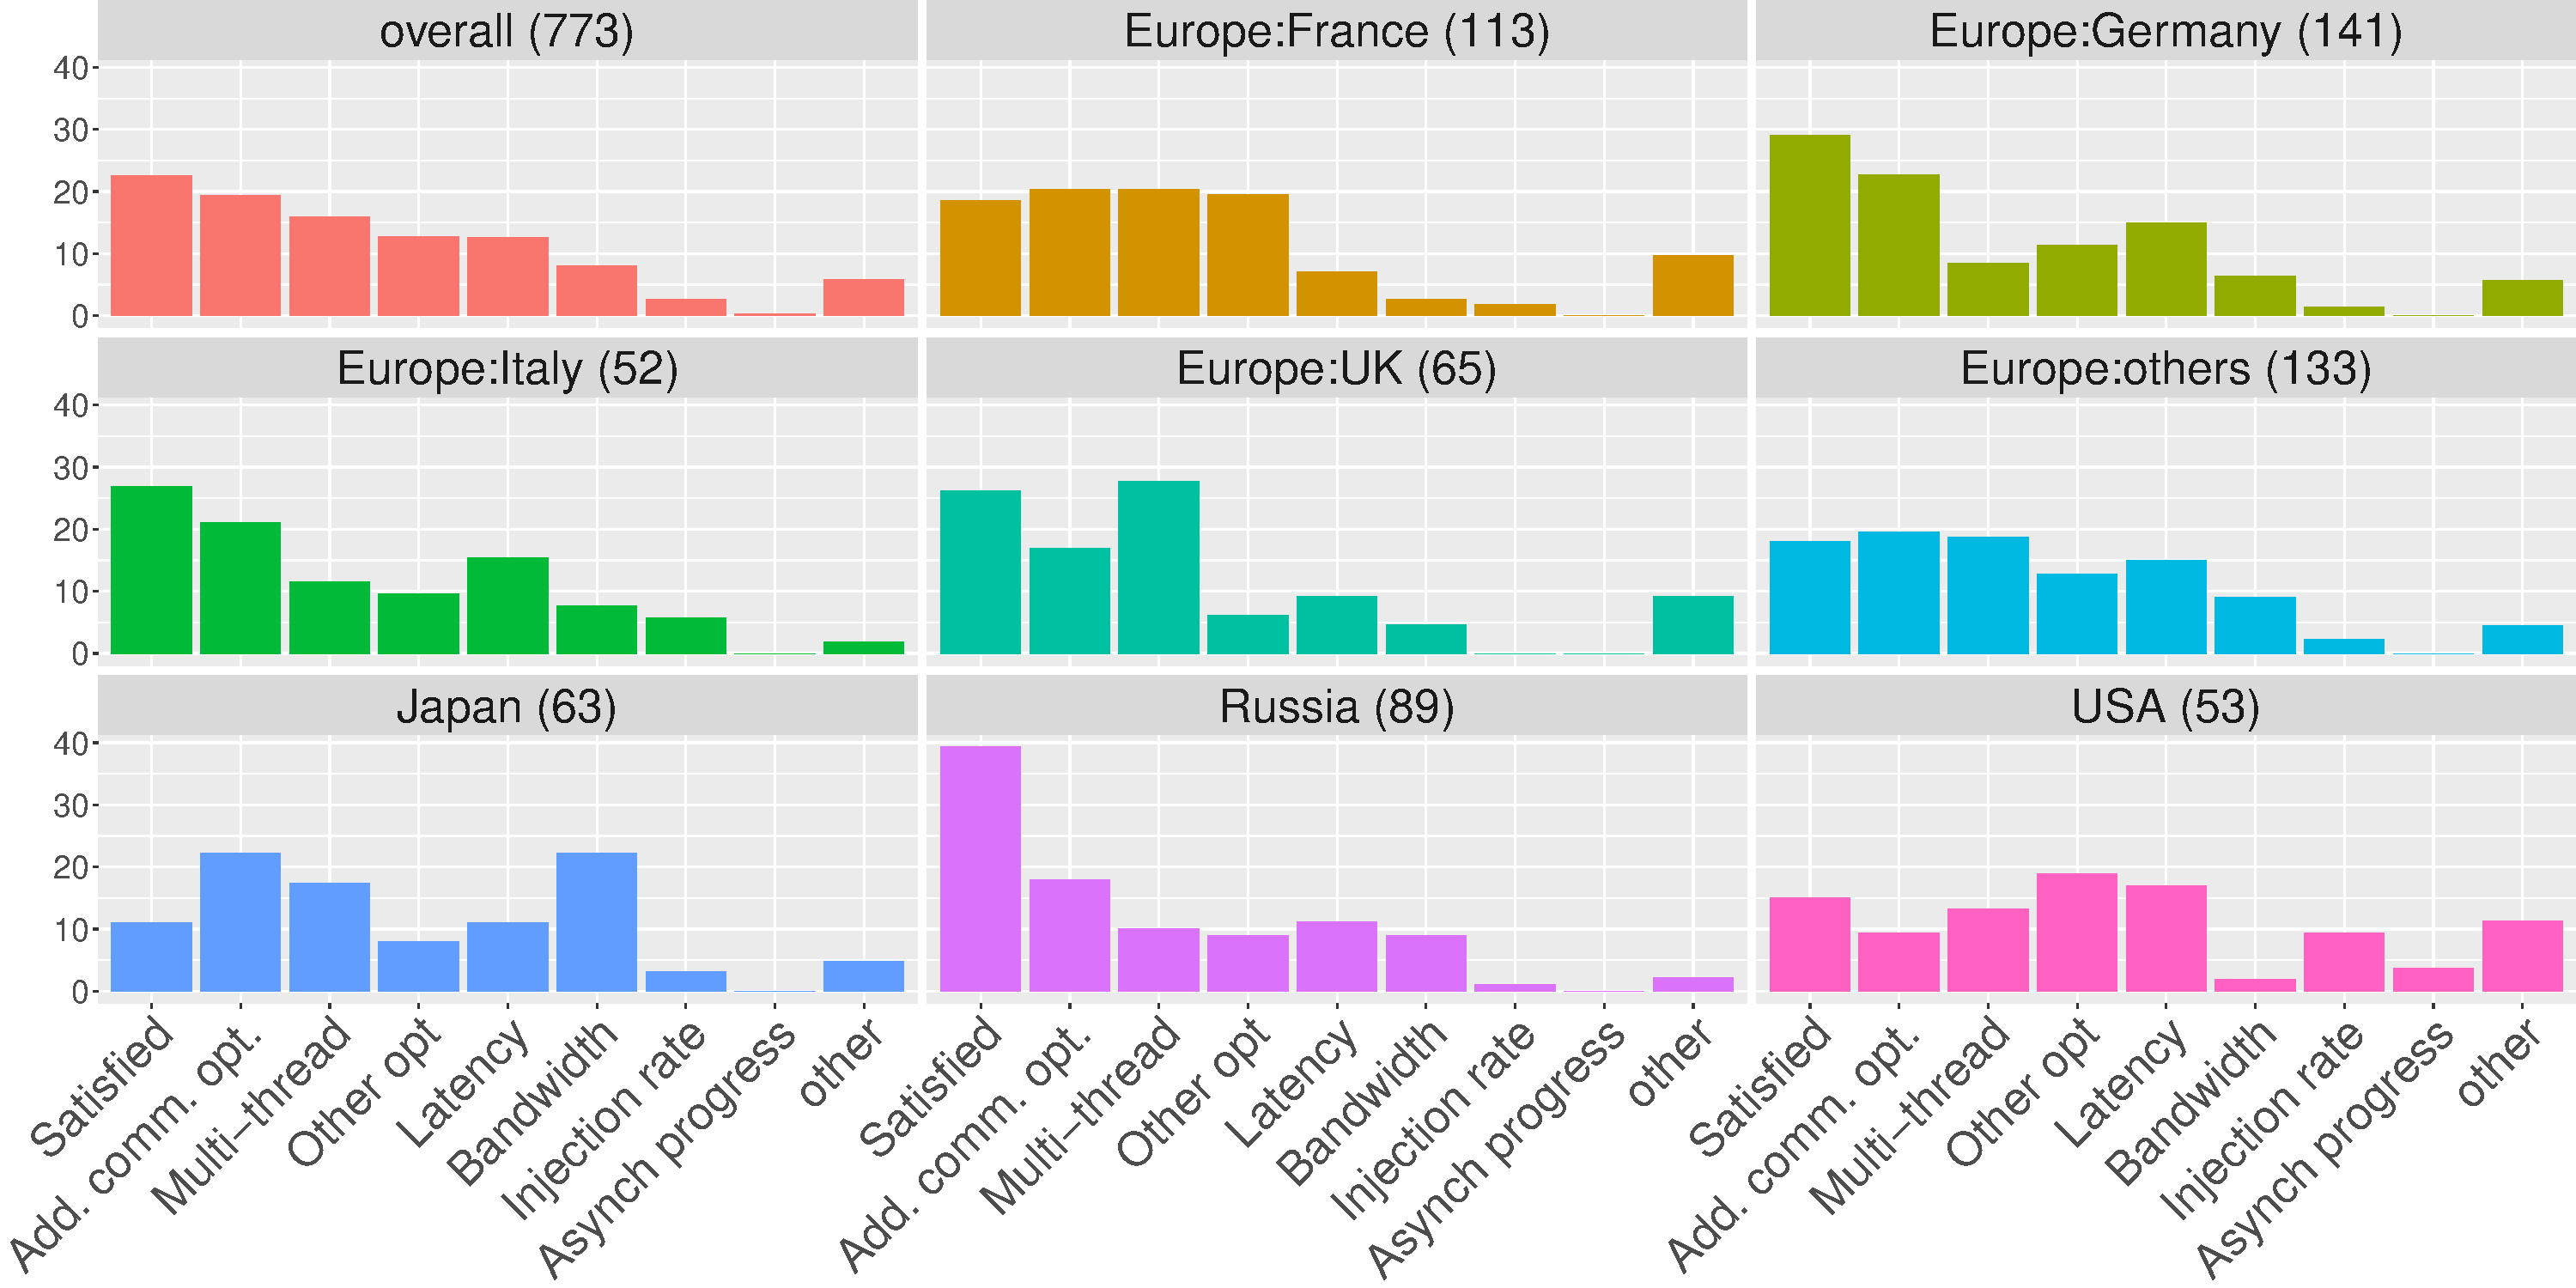
\includegraphics[width=9cm]{R-scripts/Q25.pdf}
\caption{Q25: communication aspect to improve {\it(single)}}
\label{fig:com_improvment}
\end{center}
\end{figure}

As shown in Fig.~\ref{fig:com_improvment}, in terms of capabilities of
the MPI standard and performance of the MPI implementations only a
quarter of MPI users are satisfied with the current situation. The
main concerns are related to how MPI provides general optimization
opportunities in terms of hardware capabilities such as being able to
handle the topology of the machine more efficiently. This topic is
closely followed by the concerns related to threading support, or the
integration of MPI+X, a prevalent issue in a world where a lot of
applications are trying to integrate node-level runtimes to
efficiently handle multi-core nodes.

Other optimizations such as architecture awareness or dynamic processing comes
third, but these issues are not related to the way MPI handles communications
but are identified as a bottleneck for performance as well. This represent a
shift in user awareness to hardware capabilities, and a willingness to take in
account these hardware capabilities in application/algorithm design.

Interestingly enough almost twice as many users prioritize latency
optimization vs. bandwidth optimization. Looking more closely to there
results, especially from a region perspective, pinpoints to an
interesting exception to this latency vs. bandwidth discussion.
Indeed, in Japan most users seem to be more concerned about bandwidth
rather than latency. This might be related to the last generation of
computers in Japan which are more balanced compared to other Top500
machines anbd could indicate either a raising need for bandwidth in
the region applications, or an unfounded perception of the current
Japanese platforms.

\begin{figure}[htb]
\begin{center}
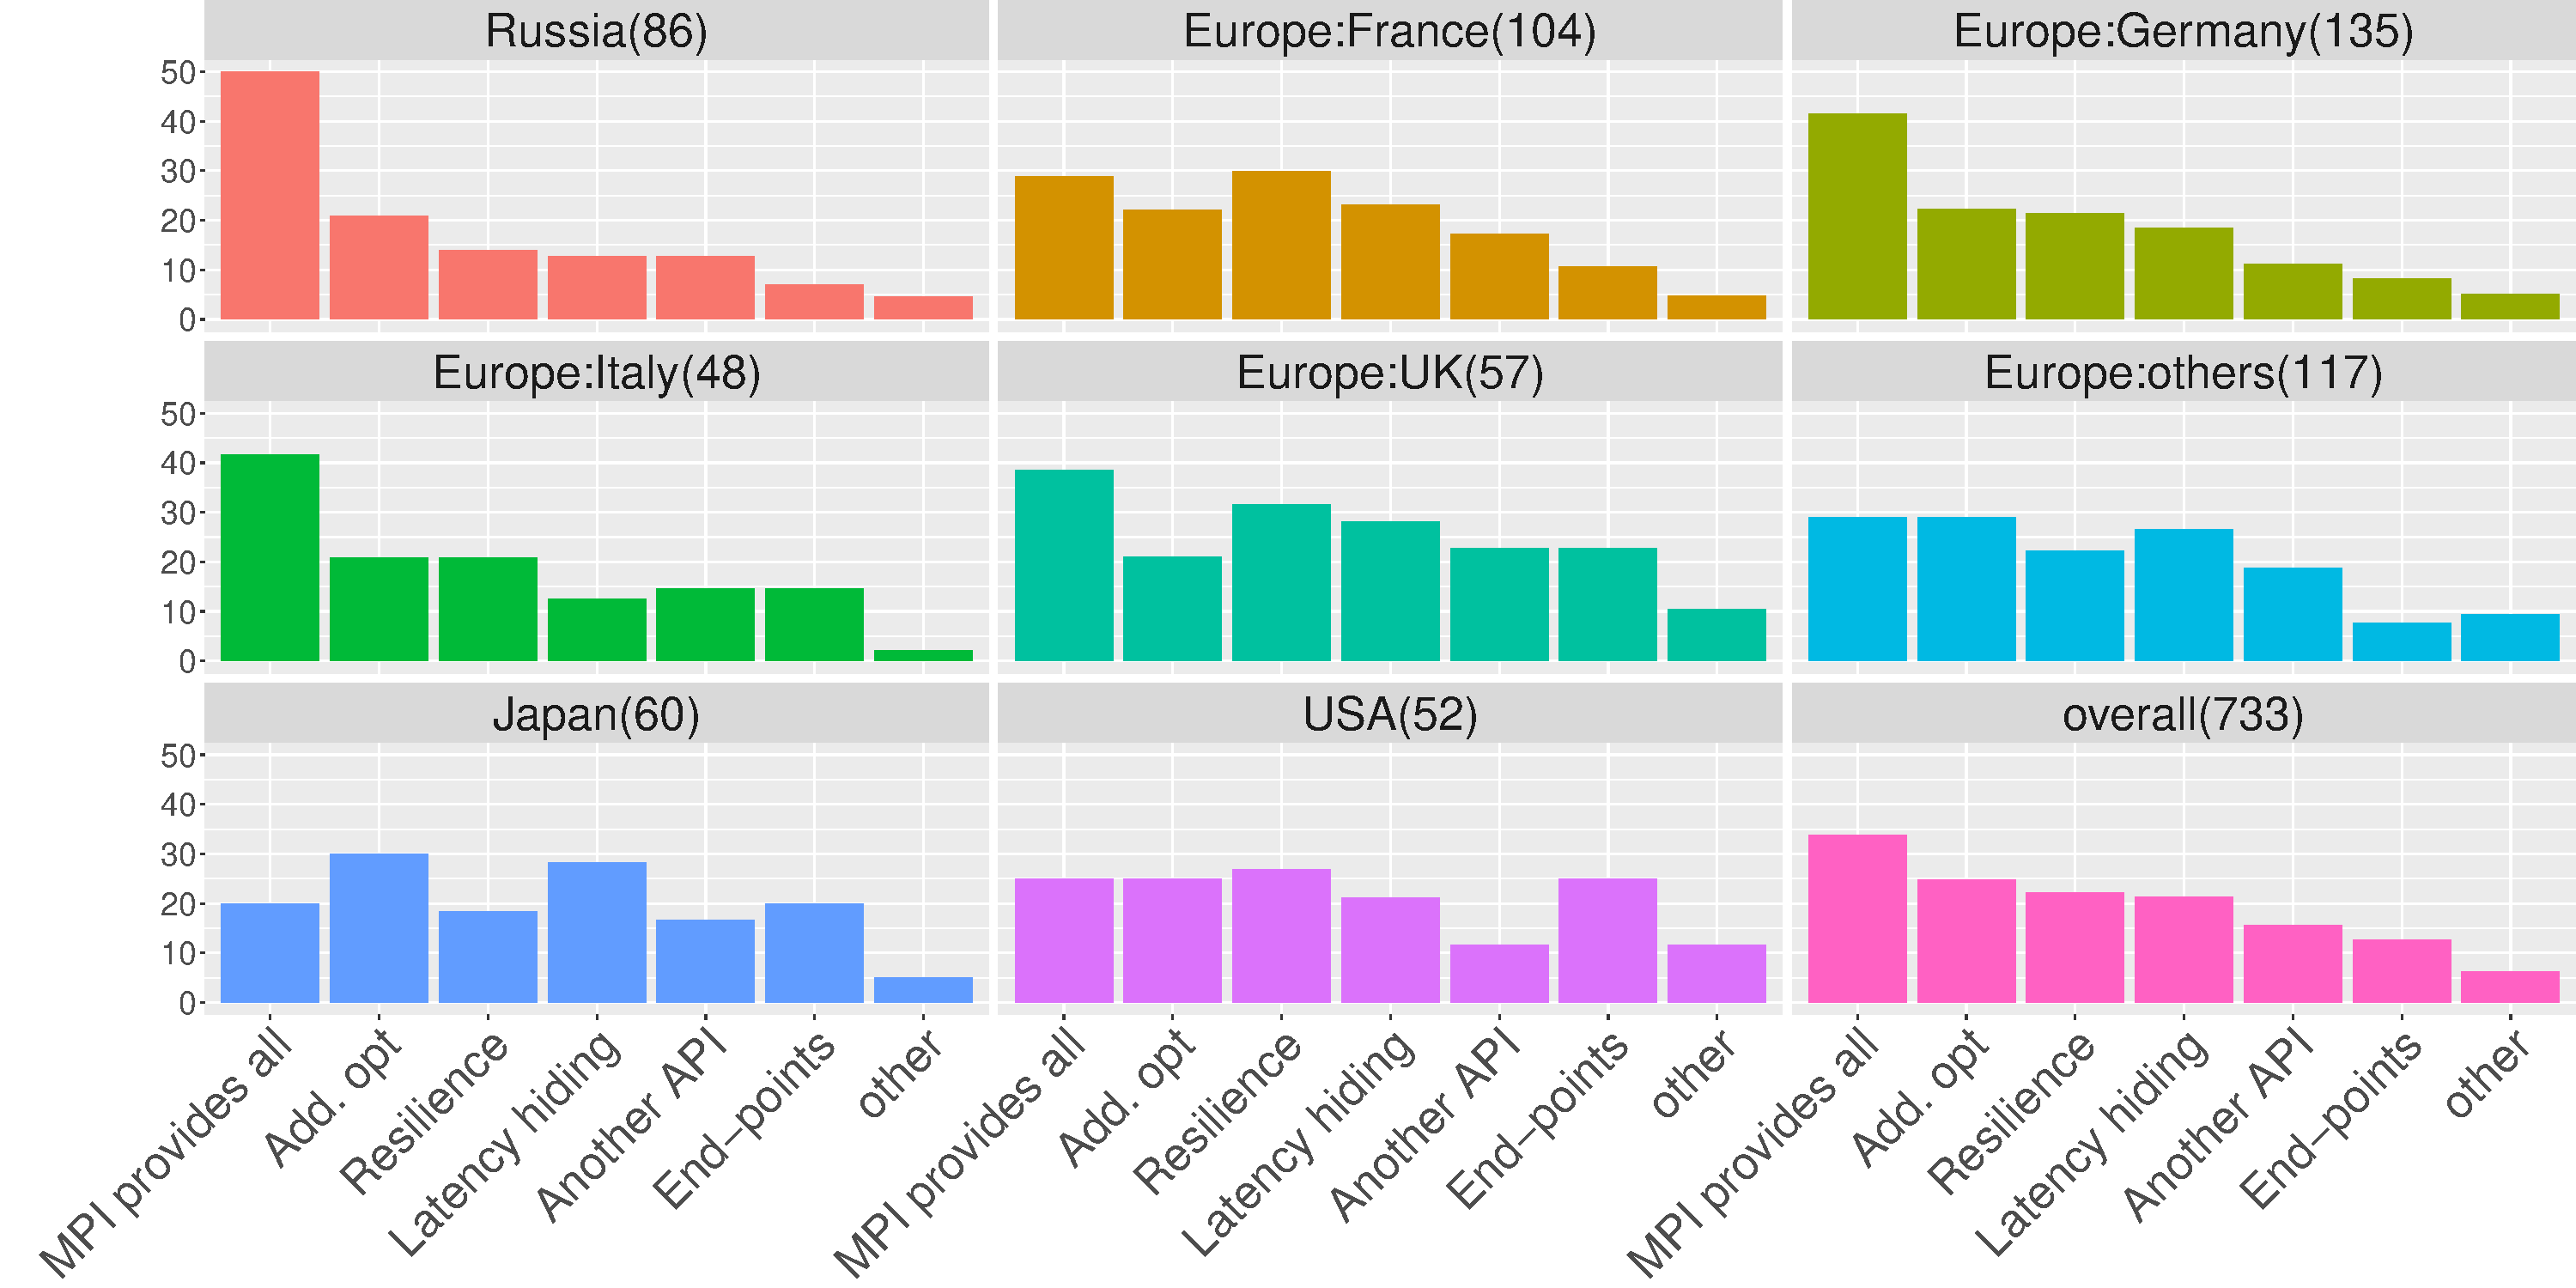
\includegraphics[width=9cm]{R-scripts/Q26.pdf}
\caption{Q26: Missing Semantic {\it(multiple)}}
\label{fig:com_sem}
\end{center}
\end{figure}

Somewhat similar to the previous question (Q25), but looking for more
precise answers, this question tackles the issue on which semantic
feature is missing from MPI (fig~\ref{fig:com_sem}). Overall a very
similar picture emerges: almost 25\% of the users are satisfied with
the current situation .

The highest given answer concerns optimization related to
communication such as topology awareness and locality management. This
is coherent with the previous question and managing efficiently the
topology seem a major concern to many users. Then comes the concerns
about the lack of resilience in MPI, a concern shared by more than
16\% of the surveyed users. Hiding latency through generalization of
asynchrony over the whole set of functions is another point raised
repeatedly. More than 10\% of the users think that a simpler and
easier API would be desirable (a topic where the discrepancy between
different regions is minimal).

Finally, the least desired feature concerns the notion of endpoints.
However taking in account the extremely technical aspect of this
question, and it's intricate evolution in the standard, it might be
possible that most people answering this question knew little, and
possible imprecisely, what this feature was exactly about.

%% It is very interesting that most countries concern about the
%% resilience. Although there are relatively big
%% disparity in the satisfaction (answering ``MPI provides all''), the
%% disparities of the other answers are smaller.

These two questions (Q25 and Q26) are also highly related to the MPI forum effort. 
%% Indeed, looking more in details at the different complains few trends emerges, small
%% enough not to become mainstream yet, but certainly providing an interesting
%% discussion ground for the future of MPI.
In fact some of these topics (such as
resilience~\footnote{https://github.com/mpi-forum/mpi-issues/issues/134,
https://github.com/mpiwg-ft} and large
counts~\footnote{https://github.com/mpi-forum/mpi-issues/issues/80}) are
currently under active discussion in the MPI Forum.
%
A short summary of frequently appearing concerns is: resilience ;
large messages ; asynchronous progress ; better accelerator support ;
internal statistics to drive further optimizations.
}
  
\subsection{Compatibility vs. Performance}

In somewhat long history of MPI, maintaining the backward
compatibility can be obstacles when to introducing new features to
enhance MPI capabilities. Fig.~\ref{fig:performance-vs-compatibility} shows the 
result of the question asking which is more important, performance or 
compatibility. Fig.~\ref{fig:compatibility} shows the percentages of
Q28 asking backward compatibility.

\begin{figure}[htb]
\begin{center}
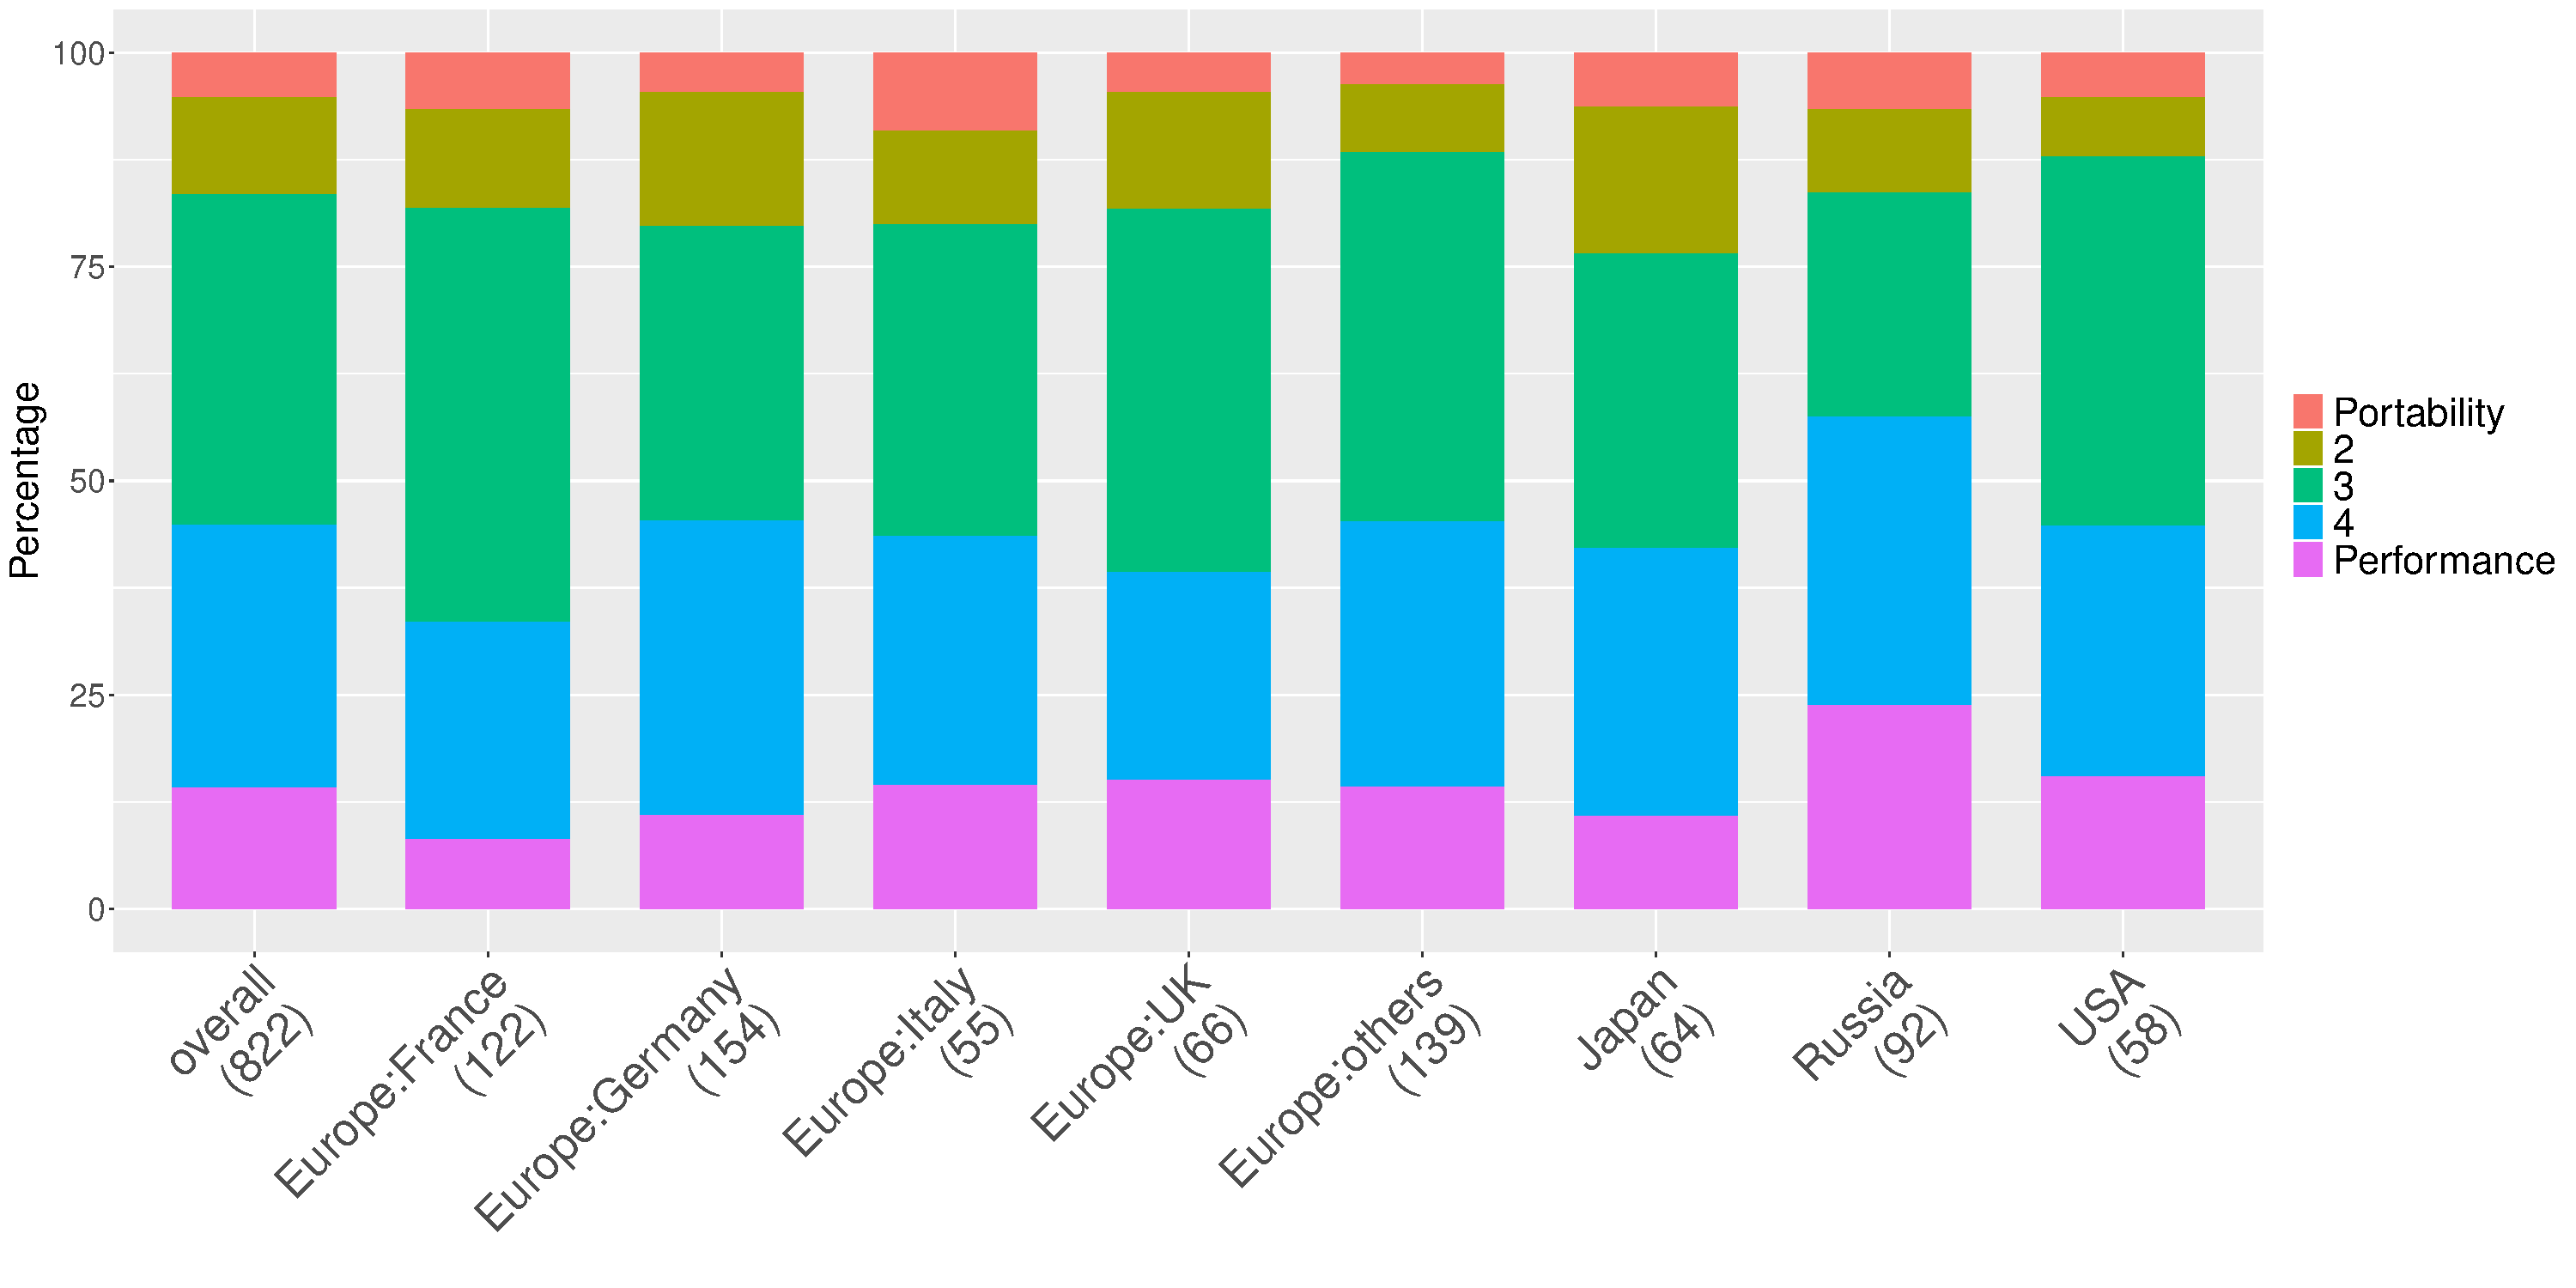
\includegraphics[width=9cm]{R-scripts/Q29.pdf}
\caption{Q29: Performance vs. Compatibility {\it(single)}}
\label{fig:performance-vs-compatibility}
\end{center}
\end{figure}

In Fig~\ref{fig:performance-vs-compatibility}, let's consider three
groups; {\it performance group} choosing \myquote{Performance} or
\myquote{4}, {\it compatibility group} choosing \myquote{Portability} or
\myquote{2}), and {\it grey group} who chose \myquote{3}. Apparently the grey
group dominates in most countries and regions (excepting Russia),
however, the performance group occupies more percentage. Regarding to
Russia, a certain percentage of Russian participants answered
\myquote{my program is too small} in Q21
(Fig.~\ref{fig:layering-mpi-calls}). If program is small enough, then
the compatibility does not cause a big problem.

\begin{figure}[htb]
\begin{center}
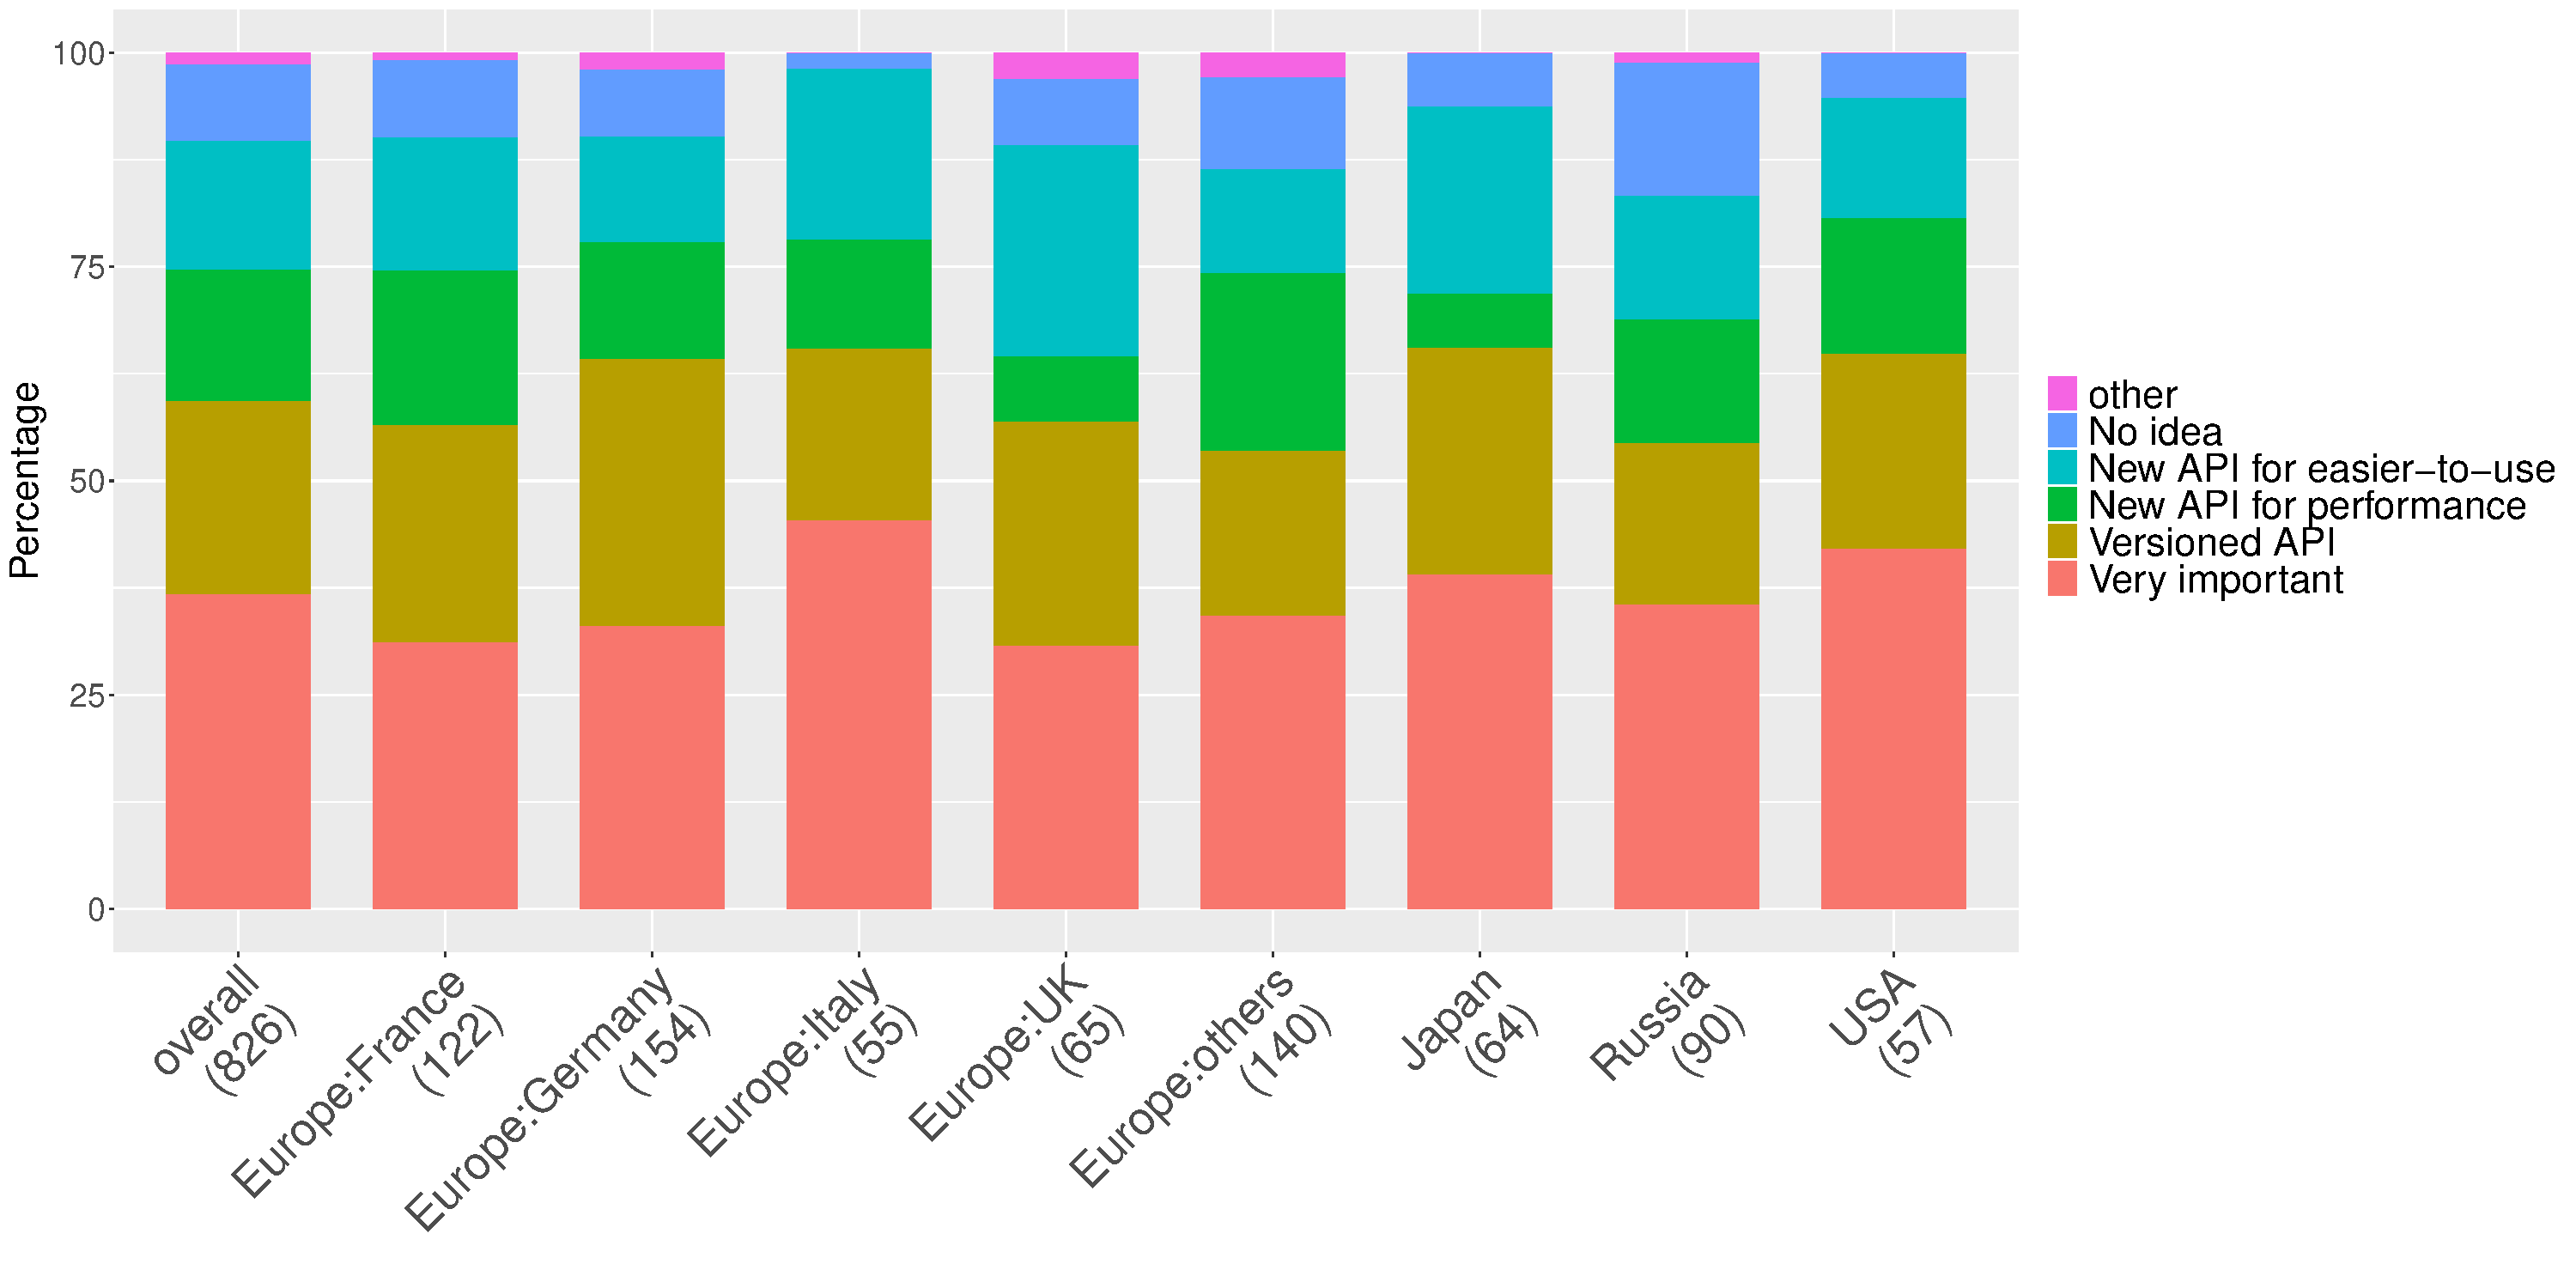
\includegraphics[width=9cm]{R-scripts/Q28.pdf}
\caption{Q28: Backward Compatibility {\it(single)}}
\label{fig:compatibility}
\end{center}
\end{figure}

As shown in Fig.~\ref{fig:compatibility}, around 40\% of participants
answered that the compatibility is very important, while the rest of
participants may accept the incompatibility conditionally. The
incompatibility forces users to update their program. The result of
Q28 may suggests that users would accept incompatibility if the users
could get some kind of benefit from the incompatible updates of MPI
specification. 

\section{Summary}

We have conducted a questionnaire survey and succeeded to gather more
than 850 participants from more than 40 countries and regions. By
analyzing the collected data, we could get several findings. As for
the MPI features, the dynamic process feature is considered not only
as a less-used feature but also a useless feature (highlighting that
the MPI programming model is seen as {\em static}). By asking several
questions how participants obtain MPI knowledge, it is revealed that
most participants read the MPI standard only partially to check the
specification of MPI functions. Instead many MPI users desire to have
practical programming guideline, online documents in
hyper-text form, and practical sample programs. Most important
(and most difficult) thing is those supplemental
documents must be up-to-dated and thorough. For the
compatibility, many MPI users may sacrifice the compatibility to get
more performance. 

All collected answers, the programs to analyze the survey data,
and all published reports are available at
{\tt \url{https://github.com/bosilca/MPIsurvey.git}}. 

\section*{Acknowledgments}

We thank to those who participated in this survey and those who
helped us to distribute the questionnaire to their local
communities. We especially thank to MPI Forum members who gave us many
significant comments on the draft questionnaire.
This research is partially supported by the
NCSA-Inria-ANL-BSC-JSC-Riken-UTK Joint-Laboratory for Extreme Scale
Computing~\cite{JLESC}.

\bibliographystyle{IEEEtran}
\bibliography{../ref}

\appendix
\section{List of Questions and Choices}
\label{app:questions}

{\small

  The followings are the list of all questions associated with
choices. The question numbers suffixed by \myquote{*} are
multiple-answer questions. The choices are followed by corresponding
abbreviations in square brackets.
\vspace{3mm}
{\scriptsize
  \begin{description}
  \item[Q1:] What is your main occupation
    \begin{inparaenum}[{\bf C}1)]
    \item College/University [Univ]
    \item Governmental institute [Gov]
    \item Hardware vendor [HW]
    \item Software vendor [SW]
    \item Private research institute [priv]
    \item Other [other]
    \end{inparaenum}
  \item[Country:] \hspace{3mm}Select main country or region of your workplace in past 5 years.
    Choose one from the country list.
  \item[Q2:] Rate your overall programming skill (non-MPI programs).
    Choose one in the range of 1 to 6. [Low-High]
  \item[Q3:] Rate your MPI programming skill.
    Choose one in the range of 1 to 6. [Low-High]
  \item[Q4*:] What programming language(s) do you use most often?
    \begin{inparaenum}[{\bf C}1)]
    \item C/C++ [C(++)]
    \item Fortran 90 or newer [\textgreater=F90]
    \item Fortran (older one than Fortran 90) [\textless F90]
    \item Python [Py]
    \item Java [Java]
    \item Other [other]
    \end{inparaenum}
  \item[Q5:] How long have you been writing computer programs (incl. non-MPI programs)?
    \begin{inparaenum}[{\bf C}1)]
    \item more than 10 years [\textgreater10]
    \item between 5 and 10 years [5-10]
    \item between 2 and 5 years [2-5]
    \item less than 2 years [\textless 2]
    \end{inparaenum}
  \item[Q6:] How long have you been writing MPI programs?
    \begin{inparaenum}[{\bf C}1)]
    \item more than 10 years [\textgreater10]
    \item between 5 and 10 years [5-10]
    \item between 2 and 5 years [2-5]
    \item less than 2 years [\textless 2]
    \end{inparaenum}
  \item[Q7*:] Which fields are you mostly working in?
    \begin{inparaenum}[{\bf C}1)]
    \item System software development (OS, runtime library, communication
      library, etc.) [OS/R]
    \item Parallel language (incl. domain specific language) [Lang]
    \item Numerical application and/or library [Num-App/Lib]
    \item AI (Deep Learning) [AI]
    \item Image processing [Image Proc]
    \item Big data [Bg Data]
    \item Workflow and/or In-situ [Workfflow]
    \item Visualization [Visualization]
    \item Tool development (performance tuning, debugging, etc.) [Tool]
    \item Other [other]
    \end{inparaenum}
  \item[Q8*:] What is your major role at your place of work?
    \begin{inparaenum}[{\bf C}1)]
    \item Research and development of application(s) [Apps]
    \item Research and development software tool(s) [Tools]
    \item Parallelization of sequential program(s) [parallelize]
    \item Performance tuning of MPI program(s) [Tuning]
    \item Debugging MPI programs [Debug]
    \item Research and development on system software (OS and/or runtime
      library) [OS/R]
    \item Other [other]
    \end{inparaenum}
  \item[Q9:] Have you ever read the MPI standard specification document?
    \begin{inparaenum}[{\bf C}1)]
    \item I read all. [All]
    \item I read most of it. [Mostly]
    \item I read only the chapters of interest for my work. [Partly]
    \item I have not read it, but I plan to. [Wish]
    \item No, and I will not read it. [No]
    \end{inparaenum}
  \item[Q10*:] How did you learn MPI?
    \begin{inparaenum}[{\bf C}1)]
    \item I read the MPI standard document. [Standard]
    \item I had lecture(s) at school. [School]
    \item I read articles found on Internet. [Internet]
    \item I read book(s). [Books]
    \item Other lectures or tutorials (workplace, conference). [Other lec.]
    \item I have not learned MPI. [Never learned]
    \item Other [other]
    \end{inparaenum}
  \item[Q11*:] Which MPI book(s) have you read?
    \begin{inparaenum}[{\bf C}1)]
    \item Beginning MPI (An Introduction in C) [Beginning MPI]
    \item Parallel Programming with MPI [Parallel Programming]
    \item Using MPI [Using MPI]
    \item Parallel Programming in C with MPI and OpenMP [Parallel
      Programming in C]
    \item MPI: The Complete Reference [MPI: Complete Ref]
    \item I have never read any MPI books [(no book)]
    \item Other [other]
    \end{inparaenum}
  \item[Q12*:] Which MPI implementations do you use?
    \begin{inparaenum}[{\bf C}1)]
    \item MPICH [MPICH]
    \item Open MPI [OMPI]
    \item Intel MPI [Intel]
    \item MVAPICH [MVA]
    \item Cray MPI [Cray]
    \item IBM MPI (BG/Q, PE, Spectrum) [IBM]
    \item HPE MPI [HPE]
    \item Tianhe MPI [Tianhe]
    \item Sunway MPI [Sunway]
    \item Fujitsu MPI [Fujitsu]
    \item NEC MPI [NEC]
    \item MS MPI [MS]
    \item MPC MPI [MPC]
    \item I do not know [No idea]
    \item Other [other]
    \end{inparaenum}
  \item[Q13:] Why did you choose the MPI implementation(s)?
    \begin{inparaenum}[{\bf C}1)]
    \item I like to use it. [I like]
    \item I was said to use it. [Said to use]
    \item I could not have any choice (the one provided by a vendor). [No choice]
    \item I am familiar with it. [Familiar]
    \item I have no special reason. [No reason]
    \end{inparaenum}
  \item[Q14*:] How do you check MPI specifications when you are writing MPI programs?
    \begin{inparaenum}[{\bf C}1)]
    \item I read the MPI Standard document (web/book). [MPI standard]
    \item I read online documents (such as man pages). [Online docs]
    \item I search the Internet (Google / Stack Overflow). [Internet]
    \item I ask colleagues. [Colleagues]
    \item I read book(s) (except the MPI standard). [Books]
    \item I know almost all MPI routines. [I know all]
    \item Other [other]
    \end{inparaenum}
  \item[Q15:] What is the most difficult part of writing an MPI program?
    \begin{inparaenum}[{\bf C}1)]
    \item Algorithm design [Algorithm]
    \item Debugging [Debugging]
    \item Domain decomposition [Decomposition]
    \item Finding appropriate MPI routines [Finding MPI routines]
    \item Implementation issue workaround [Workaround]
    \item Performance tuning [Tuning]
    \item Other [other]
    \end{inparaenum}
  \item[Q16*:] Which MPI features have you never heard of?
    \begin{inparaenum}[{\bf C}1)]
    \item Point-to-point communications [Point-to-point]
    \item Collective communications [Collectives]
    \item Communicator operations (split, duplicate, and so on) [Communicator]
    \item MPI datatypes [Datatypes]
    \item One-sided communications [One-sided]
    \item Dynamic process creation [Dyn. process]
    \item Persistent communication [Persistent]
    \item PMPI interface [PMPI]
    \item MPI with OpenMP (or multithread) [with OpenMP]
    \item Other [other]
    \end{inparaenum}
  \item[Q17*:] What aspects of the MPI standard do you use in your program in its current form?
    \begin{inparaenum}[{\bf C}1)]
    \item Point-to-point communications [Point-to-point]
    \item Collective communications [Collectives]
    \item Communicator operations (split, duplicate, and so on) [Communicator]
    \item MPI datatypes [Datatypes]
    \item One-sided communications [One-sides]
    \item Dynamic process creation [Dyn. process]
    \item Persistent communications [Persistent]
    \item MPI with OpenMP (or multithread) [with OpenMP]
    \item PMPI interface [PMPI]
    \item Other [other]
    \end{inparaenum}
  \item[Q18*:] Which MPI thread support are you using?
    \begin{inparaenum}[{\bf C}1)]
    \item MPI\_THREAD\_SINGLE [SINGLE]
    \item MPI\_THREAD\_FUNNELED [FUNNELED]
    \item MPI\_THREAD\_SERIALIZED [SERIALIZED] 
    \item MPI\_THREAD\_MULTIPLE [MULTIPLE]
    \item I have never called {\tt MPI\_INIT\_THREAD} [never used]
    \item I do not know or I do not care. [Np idea]
    \item Other [other]
    \end{inparaenum}
  \item[Q19*:] What are your obstacles to mastering MPI?
    \begin{inparaenum}[{\bf C}1)]
    \item I have no obstacles. [No obstacles]
    \item Too many routines. [Too many routines]
    \item No appropriate lecture / book / info. [No appropriate one]
    \item Too complicated and hard to understand. [Complicated]
    \item I have nobody to ask. [Nobody to ask]
    \item I do not like the API. [Dislike API]
    \item Other [other]
    \end{inparaenum}
  \item[Q20:] When you call an MPI routine, how often do you check the error code of the MPI routine  (excepting MPI-IO)?
    \begin{inparaenum}[{\bf C}1)]
    \item I rely on the default ‘Errors abort’ error handling [Default]
    \item Always [Always]
    \item Mostly [Mostly]
    \item Sometimes [Sometimes]
    \item Never [Never]
    \item Other [other]
    \end{inparaenum}
  \item[Q21:] In most of your programs, do you pack MPI function calls into their own file or files to have your own abstraction layer for communication?
    \begin{inparaenum}[{\bf C}1)]
    \item Yes, to minimize the changes of communication API. [Yes]
    \item Yes, but I have no special reason for doing that. [Yes, but no reason]
    \item No, my program is too small to do that. [No, too small]
    \item No, MPI calls are scattered in my programs. [No, scattered]
    \item Other
    \end{inparaenum}
  \item[Q22*:] Have you ever written MPI+”X” programs?
    \begin{inparaenum}[{\bf C}1)]
    \item OpenMP [OMP]
    \item Pthread [Pthread]
    \item OpenACC [OACC]
    \item OpenCL [OCL]
    \item CUDA [CUDA]
    \item No [No]
    \item Other [other]
    \end{inparaenum}
  \item[Q23:] Is there any room for performance tuning in your MPI programs?
    \begin{inparaenum}[{\bf C}1)]
    \item No, my MPI programs are well-tuned. [Well-tuned]
    \item Yes, I know there is room for tuning but I should re-write large
      part of my program to do that. [Hard to rewrite]
    \item Yes, I know there is room for tuning but I do not have enough resources to do that.
      [No resource]
    \item I think there is room but I do not know how to tune it.
      [No idea to tune]
    \item I do not have (know) tools to find performance bottlenecks.
      [Not having the tools]
    \item I have no chance to investigate.
      [No chance to investigate]
    \item I do not know how to find bottlenecks.
      [No idea to find bottlenecks]
    \item I do not know if there is room for performance tuning.
      [No idea to improve]
    \item Other [other]
    \end{inparaenum}
  \item[Q24*:] What, if any, alternatives are you investigating to
    indirectly call MPI or another communication layer by using another
    parallel language/library? 
    \begin{inparaenum}[{\bf C}1)]
    \item A framework or library using MPI. [Framework]
    \item A PGAS language (UPC, Coarray Fortran, OpenSHMEM, XcalableMP,
      ...). [PGAS]
    \item A Domain Specific Language (DSL). [DSL]
    \item Low-level communication layer provided by vendor (Verbs, DCMF,
      ...). [LL comm]
    \item I am not investigating any alternatives. [No investigation]
    \item Other [other]
    \end{inparaenum}
  \item[Q25:] If there were one communication aspect which is not enough
    in the current MPI could improve the performance of your application,
    what would you prioritize? Or is MPI providing all the communication
    semantics required by your application? If not, what is missing? 
    \begin{inparaenum}[{\bf C}1)]
    \item Latency [Latency]
    \item Message injection rate [Injection rate]
    \item Bandwidth [Bandwidth]
    \item Additional optimization opportunities in terms of communication
      (network topology awareness, etc.) [Additional comm. opt.]
    \item Optimization opportunities except communication (architecture
      awareness, dynamic processing, accelerator support, etc.) [Other opt.]
    \item Multi-threading support [Multi-thread]
    \item Asynchronous progress [Asynch progress]
    \item MPI provides all semantics I need [Satisfied]
    \item Other [other]
    \end{inparaenum}
  \item[Q26*:] Is MPI providing all the communication semantics required
    by your application? If not, what is missing? 
    \begin{inparaenum}[{\bf C}1)]
    \item Latency hiding (including asynchronous completion) [Latency hiding]
    \item Endpoints (multi-thread, sessions) [End-points]
    \item Resilience (fault tolerance) [Resilience]
    \item Additional optimization opportunities in terms of communication
      (topology awareness, locality, etc.) [Additional opt]
    \item Another API which is easier and/or simpler to use [Another API]
    \item MPI is providing all the communication semantics required by my
      application [MPI provides all]
    \item Other [other]
    \end{inparaenum}
  \item[Q27*:] What MPI feature(s) are NOT useful for your application?
    \begin{inparaenum}[{\bf C}1)]
    \item One-sided communication [One-sided]
    \item Datatypes [Datatypes]
    \item Communicator and group management [Communicator]
    \item Collective operations [Collectives]
    \item Process topologies [Topologies]
    \item Dynamic process creation [Dyn. process]
    \item Error handlers [Error]
    \item There are no unnecessary features [No]
    \item Other [other]
    \end{inparaenum}
  \item[Q28:] Do you think the MPI standard should maintain backward
    compatibility? 
    \begin{inparaenum}[{\bf C}1)]
    \item Yes, compatibility is very important for me. [Very important]
    \item API should be clearly versioned. [Versioned API]
    \item I prefer to have new API for better performance. [New API for performance]
    \item I prefer to have new API which is simpler and/or
      easier-to-use. [New API for easier-to-use] 
    \item I do not know or I do not care. [No idea]
    \item Other [other]
    \end{inparaenum}
  \item[Q29:] In the tradeoff between code portability and performance,
    which is more or less important for you to write MPI programs? 
    Choose one in the range of 1 to 6. [Portability-Performance]
  \end{description}
}}
\end{document}
